\chapter{Measures of information capacity}
%\markboth{Measures of information capacity}{Measures of information capacity}
%\addcontentsline{toc}{chapter}{Measures of information capacity}
\label{sec:infocap}

%\def\GFRE{\operatorname{GFRE}}
%\def\GFRD{\operatorname{GFRD}}
%\def\LFRE{\operatorname{LFRE}}
%
%\def\CF{\mathcal{F}}
%\def\CD{\mathcal{D}}
%\def\CF{\mathcal{F}}
%\def\CH{\mathcal{H}}
%\def\BR{\mathbb{R}}
%\def\bX{\mathbb{X}}
%\def\bx{\mathbb{x}}
%\def\bXt{\mathbb{X}^T}

\def\Fone{$\mathcal{F}$}
\def\Ftwo{$\mathcal{G}$}
\def\Ftrue{$\Theta$}
% ---

%In the last chapter we learned about the process of chosing a set of basis
%functions and the target function to obatain a numerical description, a process
%referred as \emph{featurization}.  As we discussed common characterstics of
%widely-applied radial basis in Section~\ref{sec:radial_basis_set}, the design of
%these characterstics is driven by physical and chemical intuition and is then
%tested on a variety of datasets to quantify the effectiveness of the design
%choice\cite{musil2021efficient}.  This makes the quantification dependent on a
%target property and thereby limiting the kind of insights that can be obtained..
%%creating effectiveness of the basis
%In this chapter information measures are presented that the extend the ways how we evaluate the quality of features.
%It is shown how they can be used to give different forms of insights helping with design decision in model construction and how to efficiently compute them. 

%The construction of efficient and insightful descriptors of atomic configurations has been one of the focal points of the development of data-driven applications for atomic-scale modeling~\cite{behl-parr07prl,bart+10prl,rupp+12prl,bart+13prb,de+16pccp,eick+17nips,huo2017unified,fabe+17jctc, chmiela2018towards,zhan+18prl,will+19jcp,drau19prb,chri+20jcp,van2020regularised, Ghiringhelli2015, zhu+16jcp, Gallet2013}.
In the last chapter we learned about the core ideas that underlie most of the existing atom-centred description schemes that are particularly well-suited to model additive, extensive properties, and the incorporation of geometric and atom permutation symmetries.
While incorporation of symmetries makes representations much more data efficient, it raises subtle issues of whether the mapping from structure to descriptor is injective or not~\cite{bart+13prb,vonl+15ijqc, pozd+20prl}. 
Many of the structural representations that fulfill these symmetry requirements are closely related to one another, corresponding to projections of $n$-body correlations of the atom density~\cite{will+18pccp,will+19jcp}.
Yet, comparing them is not straightforward. When used to build an interatomic potential, or to predict another atomic-scale property, representations are used together with different supervised learning schemes, so it is difficult to disentangle the interplay of descriptor, regression method, and target property that combine to determine the accuracy and computational cost of the different methods.~\cite{zuo+20jpcl}
Juxtaposing alternative choices of representations is complicated by the fact that non-linear transformations are often applied as a part of the data processing algorithm, and so it would be equally important to be able to analyze the effect of these transformations.
Efforts to compare different choices of descriptors have been mostly focused this far on a comparison of compressibility~\cite{helf+20mlst,onat+20jcp}, their ability to represent atomic structures uniquely~\cite{moussa2012comment,bart+13prb,sadeghi2013metrics,pozd+20prl}, their role in constructing a metric~\cite{zhu+16jcp,de+16pccp} and their sensitivity to perturbations of the atomic structure~\cite{pars+20mlst, onat+20jcp}.

Here we propose a strategy to compare feature spaces both in terms of their mutual information content -- which we define transparently as the ability to linearly or non-linearly reconstruct each other -- and in terms of the amount of deformation that has to be applied to match the common information between the two.
Note that the definition we use here differs from that used in information-theoretical treatments, based on Shannon entropy -- which is difficult to compute in high dimensions~\cite{torkkola2003feature}, and does not reflect as naturally the behavior of different features when used in the context of atomistic machine learning.

This strategy is demonstrated by applying it to elucidate several issues related to the behavior of density-based representations.
First, we investigate the role of the basis and of the density smearing in the practical implementation of 3-body density correlation features; we then estimate the loss of information that one incurs by truncating the description to low body-order of correlations;  finally, we discuss the role of the metric used to compare two structures, by testing the commonly used Euclidean distance against kernel-induced and Wasserstein-type metrics.
An open-source implementation of functions to compute these quantities is provided in the package \texttt{scikit-matter}\cite{goscinski2023scikit}.

%The development of computational methods that can efficiently produce quantative result that provide insights about the approximation error of representations for a given dataset has been therefore one focus of my thesis and is covered in this chapter.
%In this chapter we introduce different forms of $T$ that can give different characterization of the mutual relationship between different featurisations covering the work of Ref.~\cite{goscinski2021role}.

\section{Comparing feature spaces}
Consider a dataset $\CD=\left\{x_i\right\}$ containing $\ns$ items. For a given choice of features $\CF$, each item is described by an $\nf_\CF$-dimensional feature vector $\bx_i$. As a whole, the dataset is described by a feature matrix $\bX_\CF^\CD \in \BR^{\ns\times\nf_\CF}$.
We consider all of the feature matrices in this work to be standardized, i.e. centred and scaled so as to have zero mean and unit variance for the selected data set.
Consider a second featurization $\CF^{\prime}$. We want to be able to compare the behavior of different choices of feature spaces when representing the dataset $\CD$, e.g. which of two sets of features have more expressive power, and how much distorted is one representation relative to the other.
A schematic that depicts the strategies to compare features spaces presented in this chapter is shown in Figure~\ref{fig:gfr-scheme}.

\begin{figure}[tbhp]
\centering
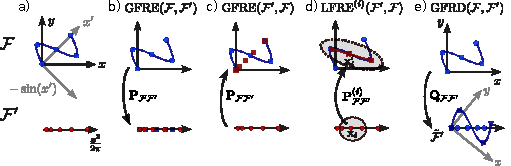
\includegraphics[width=1.0\linewidth]{fig/rof/feature-measures-scheme.pdf}
\caption{\revadd{A schematic representation of the different measures of feature-space dissimilarity we introduce in this work, discussed from left to right.
The figure considers a dataset containing five samples, embedded in a two-dimensional feature space $\CF$ and a one-dimensional feature space $\CF^{\prime}$.
As shown, the relationship between the two embeddings can involve arbitrary linear and non-linear transformations (panel a).
The global feature space reconstruction error (GFRE) defined in Equation~\eqref{eq:GFRE} amounts to finding the best linear mapping between the two feature spaces.
This measure is not symmetric: in this example the $\GFRE(\CF,\CF^{\prime})$ (panel b) is smaller than the $\GFRE(\CF^{\prime},\CF)$ (panel c), since $\CF$ contains an additional nonzero dimension.
The local version of the reconstruction error (LFRE) defined in Equation~\eqref{eq:LFRE} makes it possible to probe whether a non-linear map exists between the two spaces: in this case, the sinus function can be approximated in  neighborhood of each sample $\bx_i$ by a linear map $\bP{\CF}{\CF^{\prime}}^{(i)}$  defined in Equation~\eqref{eq:xtilde_lle}; by treating each neighborhood separately  it is possible to achieve a low $\LFRE(\CF^{\prime},\CF)$ (panel d). 
Finally, the global feature space reconstruction distortion (GFRD) defined in Equation~\eqref{eq:GFRD} determines whether the two featurizations are connected by an orthogonal transformation $\bQ{\CF}{\CF^{\prime}}$ defined in Equation~\eqref{eq:proc-ff1}, by finding the best alignment between $\CF$ and the approximation of $\CF^{\prime}$ that can be obtained as a linear projection of $\CF$.
Even though $\GFRE(\CF,\CF^{\prime})$ is small, one of the components of $\CF$ is scaled down to zero, resulting in a large value of $\GFRD(\CF,\CF^{\prime})$ (panel e).}}
\label{fig:gfr-scheme}
\end{figure}

\subsection{Global feature space reconstruction error}

As a simple, easily-interpretable measure of the relative expressive power of $\CF$ and $\CF^{\prime}$, we introduce the global feature space reconstruction error $\GFRE^\CD(\CF,\CF^{\prime})$, defined as the mean-square error that one incurs when using the feature matrix $\bX_\CF$ to linearly regress $\bX_{\CF^{\prime}}$. 
In this work we compute the $\GFRE$ by a 2-fold split of the dataset, i.e. compute the regression weights $\bP{\CF}{\CF^{\prime}}$ over a train set $\CDtr$ composed of half the entries in $\CD$,
\begin{equation}
\begin{split}
\bP{\CF}{\CF^{\prime}}= &
\underset{\bP{}{}\in\BR^{\nf_{\CF}\times\nf_{\CF^{\prime}}}}{\operatorname{argmin}}
\norm{\bX^{\CDtr}_{\CF^{\prime}} - \bX^{\CDtr}_{\CF} \bP{}{}  }\\
=&\left({\bX_{\CF}^{\CDtr}}^T \bX_{\CF}^{\CDtr}\right)^{-1}
(\bX_{\CF}^{\CDtr})^T\bX_{\CF^{\prime}}^{\CDtr}
\end{split}\label{eq:proj-ff1}
\end{equation}
and then compute the error over the remaining test set $\CDte$
\begin{equation}
\GFRE^\CD(\CF,\CF^{\prime}) = \sqrt{{\norm{\bX^{\CDte}_{\CF^{\prime}} - \bX^{\CDte}_{\CF} \bP{\CF}{\CF^{\prime}}  }^2}/\ns_\test},
\label{eq:GFRE}
\end{equation}
averaging, if needed, over multiple random splits.  The $\GFRE$ is a positive quantity, which is equal to zero when there is no error in the reconstruction, and that is usually bound by one\footnote{This is due to the fact that feature matrices are standardized, and so $\norm{\bX^{\CDte}_{\CF^{\prime}}}/\ns_\test $ is of the order of one}.
For numbers of features larger than $\ns_\train$, the covariance matrix is not full rank, and one needs to compute a pseudoinverse. Without loss of generality, one can regularize the regression to stabilize the calculation. In this paper, we computed the pseudoinverse by means of a singular value decomposition, and we determined the optimal regularization in terms of the truncation of the singular value spectrum, using 2-fold cross-validation over the training set to determine the optimal truncation threshold. Often, it is also useful to observe the behavior of the $\GFRE$ in the absence of any regularization: overfitting is in itself a signal of the instability of the mapping between feature spaces.
In general, $\GFRE^\CD(\CF,\CF^{\prime})$ is not symmetric. If $\GFRE^\CD(\CF,\CF^{\prime})\approx\GFRE^\CD(\CF^{\prime},\CF)\approx 0$, $\CF$ and $\CF^{\prime}$ contain similar types of information; if $\GFRE^\CD(\CF,\CF^{\prime})\approx 0$, while $\GFRE^\CD(\CF^{\prime},\CF)>0$, one can say that $\CF$ is more descriptive than $\CF^{\prime}$: this is the case, for instance, one would observe if $\CF^{\prime}$ consists of a sparse version of $\CF$, with some important and linearly-independent features removed; finally, if  $\GFRE^\CD(\CF,\CF^{\prime})\approx\GFRE^\CD(\CF^{\prime},\CF)>0$, the two feature spaces contain different, and complementary, kinds of information and it may be beneficial to combine them to achieve a more thorough description of the problem.

\subsection{Global feature space reconstruction distortion}

The feature space reconstruction error gives insights into whether a feature space can be inferred by knowledge of a second one. However, having both a small $\GFRE^\CD(\CF,\CF^{\prime})$ and $\GFRE^\CD(\CF^{\prime},\CF)$ does not imply two feature spaces are identical. Even though they contain similar amounts of information, one feature space could give more emphasis to some features compared to the other, which can eventually result in different performance when building a model.
To assess the amount of distortion of $\CF^{\prime}$ relative to $\CF$, we introduce the global feature space reconstruction distortion $\GFRD^\CD(\CF,\CF^{\prime})$.
To evaluate it, we first compute the singular value decomposition of the projector Equation~\eqref{eq:proj-ff1}, $\bP{\CF}{\CF^{\prime}}\approx\bU \bSIG \bV^T$, and then use it to reduce the two feature spaces to a common basis, in which the reconstruction error is zero, because the residual has been discarded
\begin{equation}
\bXt_{\CF} = \bX_{\CF}\bU \quad  \bXt_{\CF^{\prime}} = \bXt_{\CF} \bSIG.
\end{equation}
When the second feature space $\CF^{\prime}$ has a lower dimensionality than $\CF$, some combinations of the starting features are not used to compute $\tilde{\CF}^{\prime}$. 
In this case, we pad $\bSIG$ with zeros, so that $\tilde{\CF}^{\prime}$ has the same dimensionality $\nf_{\CF}$ as the starting space. This choice ensures that the GFRD takes the same value it would have in the case $\CF^{\prime}$ had the same dimensionality as $\CF$, but lower rank. 
In the opposite case, with $\nf_{\CF}<\nf_{\CF}^{\prime}$, padding $\bSIG$ and $\bU$ with zeros, or truncating $\bV$, yields the same $\GFRD$.


We can then address the question of whether $\bXt_{\CF}$ and $\bXt_{\CF^{\prime}}$ are linked by a unitary transformation (in which case the $\GFRD$ should be zero), or there is a distortion involved.
A possible answer involves solving the orthogonal Procrustes problem~\cite{scho66pm} -- i.e. finding the orthogonal transformation that ``aligns``  as well as possible $\bXt_{\CF}$ to $\bXt_{\CF^{\prime}}$:
\begin{equation}
\begin{split}
  \bQ{\CF}{\CF^{\prime}} =& \underset{\bQ{}{} \in \mathbb{U}^{\nf\times\nf}}{\operatorname{argmin}}
\norm{\bXt^{\CDtr}_{\CF^{\prime}} - \bXt^{\CDtr}_{\CF} \bQ{}{}  }\\
=&\tilde{\bU}\tilde{\bV}^T,
\end{split}\label{eq:proc-ff1}
\end{equation}
where $\tilde{\bU}\tilde{\bSIG}\tilde{\bV}^T = (\bXt_{\CF}^{\CDtr})^T \bXt^{\CDtr}_{\CF^{\prime}}$ .
The amount of distortion can then be computed by assessing the residual on the test set,
\begin{equation}
\GFRD^\CD(\CF,\CF^{\prime}) = \sqrt{{\norm{{\bXt}^{\CDte}_{\CF^{\prime}} - {\bXt}^{\CDte}_{\CF} \bQ{\CF}{\CF^{\prime}}  }^2}/\ns_\test}. \label{eq:GFRD}
\end{equation}
If desired, the error can be averaged over multiple random splits of the reference data set $\CD$.

\subsection{Local feature space reconstruction error}

A downside of the global feature comparison schemes introduced above is that the linear nature of the regression means that they cannot detect if $\CF$ and $\CF^{\prime}$ contain analogous information, but differ by a non-linear transformation.
In the next Section we discuss how one can generalize the schemes to use kernel features, that can also be used to detect non-linear relationships between the original feature spaces.
An alternative approach is to compute a local version of the feature space reconstruction error, $\LFRE^\CD(\CF,\CF^{\prime})$, loosely inspired by locally-linear embedding~\cite{rowe-saul00science}. 
To compute the LFRE, a local regression is set up, computed in the $k$-neighborhood $\CDki$ around sample $i$  -- the set of $k$ nearest neighbors of sample $i$, based on the Euclidean distance between the samples in $\CF$ -- to reproduce the $\CF^{\prime}$ features using $\CF$ as input features, centred around their mean values $\bar{\bx}_{\CF^{\prime}}$ and $\bar{\bx}_{\CF}$.


A local embedding of $\bx_i$ is determined as
\begin{equation}
\tilde{\bx}^{\prime}_i = \bar{\bx}_{\CF^{\prime}} + (\bx_i - \bar{\bx}_{\CF})\bP{\CF}{\CF^{\prime}}^{(i)},\label{eq:xtilde_lle}
\end{equation}
where $\bP{\CF}{\CF^{\prime}}^{(i)}$ contains the regression weights computed from $\CDki$.
The local feature space reconstruction error is given by the residual discrepancy between the $\CF^{\prime}$ counterpart of the $i$-th point and its local embedding~\eqref{eq:xtilde_lle}:
\begin{equation}
\LFRE^\CD(\CF,\CF^{\prime}) = \sqrt{\sum_i \norm{\bx^{\prime}_i - \tilde{\bx}^{\prime}_i}^2/{\ns_\test}}.
\label{eq:LFRE}
\end{equation}
Inspecting the error associated with the reconstruction of individual points can reveal regions of feature space for which the mapping between $\CF$  and $\CF^{\prime}$ is particularly problematic. 
Similarly, one can compute a local version of $\GFRD$, that could be useful to detect strong local distortions that might indicate the presence of a singularity in the mapping between two feature spaces.

% Content:
% - Duality of descriptor + similarity/metric induces metric/similarity + feature space
% - By using the dot product a feature space + 2-Minkowski distance is induced
% - For high dimensional spread atomic structures, the 2-Minkowski distance cannot capture the relationship between disconnected clusters. This disconnectivity can leads to higher model variance in regression tasks, since the weights can be optimized independent from each other.
% - This disconnectivity can be solved with a metric that captures more global structures as the wasserstein distance
% - While not explicitly mentioned in literature, discrete versions of the Wasserstein distance have been used by using the 2-Minkowski distance with sorted descriptors. derivation ....

%\subsection{Hidden feature space reconstruction error}

%While the previous measures focus on the information contained in the features, the hidden feature space reconstruction error ($\textrm{HFRE}$) captures the coding efficiency of features important for sparsity.
%is that it cannot express how efficient information of a dataset is encoded in the features such that $\GFRE(\CF,\CF^{\prime}) > \GFRE(\CF^{\prime},\CF)$ cannot indicate if the additional information in $\CF^{\prime}$ is relevant.
%For an actual test we need to define the relevant the information of the dataset $\mathbf{z}$ which is in the case of the displaced methane dataset the distance of the pulled hydrogen atom from the central carbon atom $\mathbf{z}_{\textrm{H}}$.
%For every feature a scalar regression weight is determined to regress the hidden information vector $\mathbf{z}$
%\begin{equation}
%\tilde{\mathbf{z}}_j = \bar{\mathbf{z}} + (\mathbf{f}_j - \bar{\mathbf{f}}_{\CF})p_{\CF \mathcal{Z}}^{(j)}.\label{eq:xtilde_lle}
%\end{equation}
%The final measure is then expressed as regression error
%\begin{equation}
%\textrm{HFRE}^\CD(\CF,\mathcal{Z}) = \sqrt{\sum_j \norm{\mathbf{z} - \tilde{\mathbf{z}}_j}^2/\ns_\test}.
%\end{equation}

\subsection{Bending space: comparing induced feature spaces}

It is often possible to substantially improve the performance of regression or dimensionality reduction algorithms, without explicitly changing the feature vectors. This can be achieved by introducing a (non-linear) similarity measure to compare $\bx_i$, which takes the form of a kernel function $k(\bx,\bx^{\prime})$, or a dissimilarity measure which takes the form of a distance $d(\bx,\bx^{\prime})$.

Let us recall that a positive-definite kernel induces a kernel distance by the relation\cite{scholkopf2001kernel}
\begin{equation}
    d_k(\bx,\bx^{\prime})^2 = k(\bx,\bx) + k(\bx^{\prime},\bx^{\prime}) -2k(\bx,\bx^{\prime}),
    \label{eq:kernel_distance_relation}
\end{equation}
and that any negative-definite distance can be used to build positive-definite kernels such as the substitution kernel\cite{haasdonk2004learning}
\begin{equation}
k_d^{\mathbf{x}_0}(\bx,\bx^{\prime}) = -\frac12(d(\bx,\bx^{\prime})^2 - d(\bx,\bx_0)^2 - d(\bx_0,\bx^{\prime})^2),  \bx_0\in\CF \label{eq:k-0}
\end{equation}
or the radial basis function (RBF) kernel
\begin{equation}
k_d^{\textrm{RBF}}(\bx,\bx^{\prime}) = \exp(-\gamma d(\bx,\bx^{\prime})^2),\quad \gamma\in\BR_+ \label{eq:k-rbf}
\end{equation}

A positive definite kernel induces a feature space $\CH$, commonly known as reproducing kernel Hilbert space (RKHS), in which the similarity measure can be expressed as a dot product:
\begin{equation}
    k(\bx,\bx^{\prime}) = \bphi(\bx)\cdot\bphi(\bx^{\prime}),\quad \bx,\bx^{\prime}\in\mathcal{F},\,\, \bphi:\mathcal{F}\rightarrow\CH.
\end{equation}
While in general $\bphi(\bx)$ is not known, for a given dataset $\CD$ it is possible to approximate the RKHS features by using a kernel principal component analysis~\cite{scholkopf1997kernel}. Since linear regression in RKHS features is equivalent to kernel ridge regression, we simply use kernel features computed on the training  dataset $\CDtr$ to reduce the problem of comparing kernel (or distance) induced features to that of comparing explicit features, and use $\GFRE$ and $\GFRD$ as defined in Eqs.~\eqref{eq:GFRE} and~\eqref{eq:GFRD}. 
It is possible to re-formulate these measures in an explicit kernelized form, as well as to compute low-rank approximations of the kernel to reduce the computational cost for very large datasets (see e.g. Ref.~\citenum{helf+20mlst} for a pedagogic discussion). In this paper we simply use the explicit RKHS features, that can be obtained by diagonalizing the kernel matrix $\bK = \bU \bLAM \bU^T$, with $K_{ij} = k(\bx_i, \bx_j)$, and defining
\begin{equation}
\bX_\CH = \bU \bLAM^{-1/2},
\end{equation}
which is then standardized as we do for any other set of features. 
To define a feature space associated with a metric, rather than a kernel, we first center the squared distance matrix (which is equivalent to computing a substitution kernel analogous to Equation~\eqref{eq:k-0}) and then proceed similarly by diagonalizing the resulting matrix. 

%Most dominantly the dot product or exponential kernels have been used for regression of atomic properties.
%We just say that we do this to map the problem of comparing metrics to a problem of comparing features

% Comparison methods between induced features
%A feature space $\Phi^{\mathcal{D}_B^{(\nu)}}$ is compared to a $\Phi^{\CH}$ compared by how much information about the dataset $\mathcal{D}$ is contained relative to another feature spaces.
%This is expressed in the reconstruction error of one feature space to the other

\subsection{Dataset selection}

We use four different datasets, chosen to emphasize different aspects of the problem of representing atomic structures: A \textit{random methane} dataset consisting of different random displacements of the four hydrogen atoms around the central carbon atom to cover the complete configurational space of \ce{CH4} structures; A \textit{carbon} dataset of approximately $10^{\prime}000$ minimum energy carbon structures, obtained as the result of ab initio random structure search~\cite{pick-need11jpcm, pickard-carbon}, as an example for a realistic dataset of condensed phase structures; A \textit{degenerate methane} dataset composed of two groups of methane structures (which we refer to as $\mathcal{X}^+$ and $\mathcal{X}^-$), each associated with a 2D manifold parameterised by two parameters $(u,v)$: structures with $v=0$ in the two manifolds have exactly the same C-centred 3-body correlations, despite being different (as discussed in Ref.~\citenum{pozd+20prl});  A \textit{displaced methane} dataset, which consists in an ideal, tetrahedral \ce{CH4} geometry with one hydrogen atom pulled away from the central carbon atom, as an example of a set of structures that are distinguished by a clearly identifiable structural feature, here the \ce{C-H} distance.


\begin{figure*}
    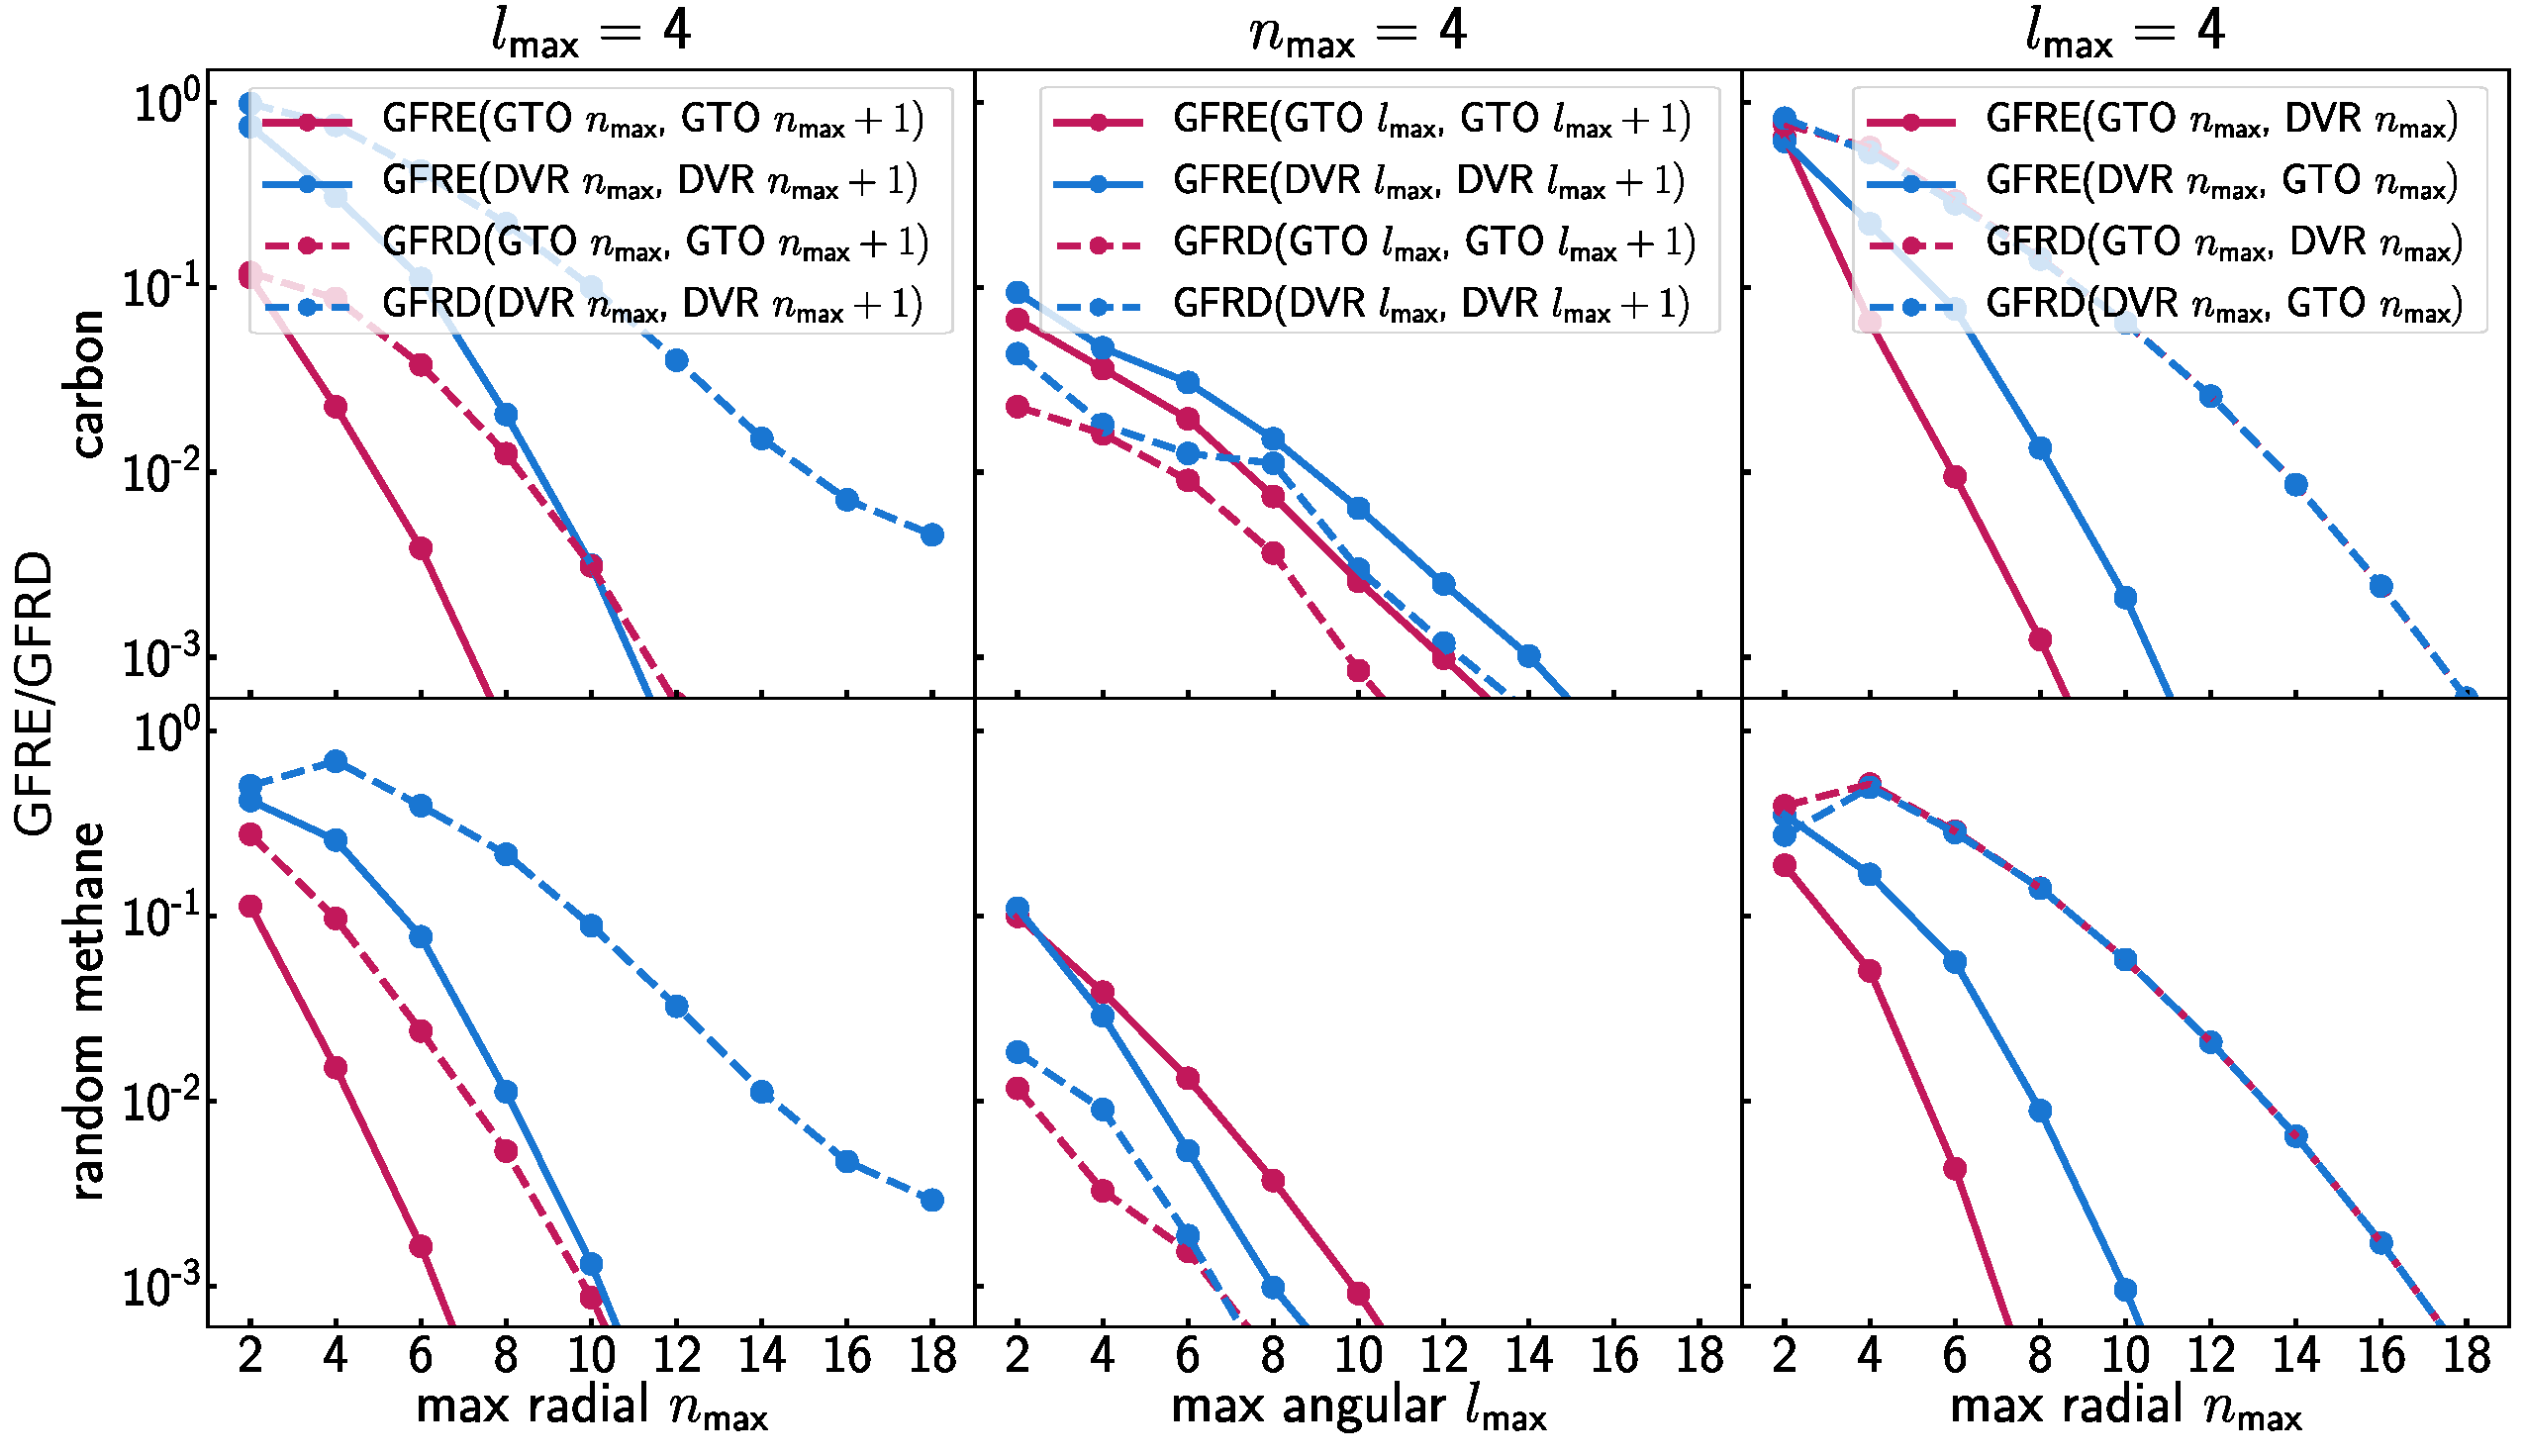
\includegraphics[width=0.9\linewidth]{fig/rof/soap_convergence-carbon_methane-inkscaped.pdf}
    \caption{Comparison of the GFRE and GFRD for increasing numbers of radial (left, with fixed $\lmax=4$) and angular (middle, with fixed $\nmax=4$) basis functions.  On the right, an explicit comparison of the two basis sets in terms of $\GFRE(\text{GTO},\text{DVR})$, $\GFRE(\text{DVR},\text{GTO})$ and the corresponding measures of distortion.}
    \label{fig:soap-convergence}
\end{figure*}


\section{Comparing ACDC representations}

While different discretizations of the abstract vectors on a basis  are a matter of computational convenience and affect the computational cost of different approaches~\cite{zuo+20jpcl}, but their descriptive power becomes equivalent in the limit of a complete basis set. 
We demonstrate the use of the GFRE, LFRE and GFRD to assess with quantifiable measures the effect of some of the different choices one can make when designing a representation.
%address some open questions concerning the construction and use of this kind of representations.

\subsection{SOAP and BPFS}
\label{sub:hypers}
We begin by considering two practical realizations of atom-centred symmetrized features of order $\nu=2$ in Equation~\eqref{eq:soap} as implemented in \texttt{librascal}\cite{LIBRASCAL}, and the BPSF\cite{behl11jcp} as implemented in the n2p2 package\cite{singraber2019parallel}. 
%In the SOAP representation the atom-centred density is written as a sum of Gaussians with finite width $\sigmag$, and the density is expanded in a basis that is a product of spherical harmonics $Y^l_m(\bxhat)\equiv\rep<\bxhat||lm>$ and a radial basis $R_n(x)\equiv\rep<x||n>$,
%\begin{equation}
%\rep<nlm||A; \rho_i> = \sum_j \int \D{\bx}
%\rep<n||x> \rep<lm||\bxhat>
%\rep<\bx-\br_{ji}||g>, \label{eq:nlm-rho}
%\end{equation}
%where $\br_{ji}=\br_j-\br_i$.
We consider two different basis sets here, Gaussian-type orbitals (GTO)
\begin{subequations}
\begin{gather}
  R_n^\textrm{GTO} = N_n r^{n}\exp(-b_nr^2),\\
\text{with }N_n=\frac2{\sigma_n^{2n+3}\Gamma((n+3)/2)},\quad b_n = 1/(2\sigma_n),\quad \sigma_n = r_c\,\textrm{max}(\sqrt{n},1)/\nmax,
\end{gather}
\end{subequations}
that are orthogonalized with respect to each other,
and a discrete variable representation (DVR) basis
\begin{equation}
R_n^\textrm{DVR}= \sqrt{w_n}\delta(r-r_n)
\end{equation}
where $r_n$ are Gaussian quadrature points and $w_n$ their corresponding weights.
For both bases, the integral~\eqref{eq:radial_expansion} can be evaluated analytically, and the density coefficient computed as a sum over the neighbors of the $i$-th atom.
%The invariant SOAP features are then computed as specified in Equation~\eqref{eq:soap},
%\begin{equation}
%\label{eq:SOAP}
%\rep<nn^{\prime}l||\frho_i^2> = 
%\sum_m  \frac{{(-1)}^m }{\sqrt{2l+1}}  \rep<nlm||\frho_i> \rep<n^{\prime}l(-m)||\frho_i>
%\end{equation}


\begin{figure*}
    \includegraphics[width=0.9\linewidth]{fig/rof/sigma_radial_scaling_cutoff_comparison-gfrd-gto_dvr-methane_carbon-inkscaped-v2.pdf}
    \caption{Comparison of the GFRE (top) and GFRD (bottom) a),b) for different smearing  $\sigma_G$ ($r_\text{c}=4\,$\AA{}) c),d) for different cutoff values ($\sigmag=0.5\,$\AA), and e),f) for different radial scaling exponents ($r_\text{c}=4\,$\AA{}, $\sigmag=0.5\,$\AA). For all comparisons $(\nmax,\lmax) = (10,6)$ were used. The feature specified by the row is used to reconstruct the feature specified by the column.}
    \label{fig:soap-sigma-radial-body}
\end{figure*}

Even though they can be seen as a projection on an appropriate basis of the symmetrized atom density that underlies SOAP~\cite{will+19jcp}, BPSF are usually computed as a sum over tuples of neighboring atoms of functions of interatomic angles and distances. Among the many functional forms that have been proposed~\cite{behl11pccp} we consider the two-body functions
%
\begin{equation}
    G^{(2)}_i = \sum_j e^{-\eta (r_{ji} - R_s)^2} \cdot f_c (r_{ji}), \label{eq:g2}
\end{equation}
and the three-body functions
\begin{equation}
    G^{(3)}_i = 2^{1-\zeta} \sum_j \sum_{k \neq j } (1 + \lambda \cdot \cos \hat{\br}_{ij}\cdot\hat{\br}_{ik})^{\zeta} \cdot
    e^{-\eta (r_{ji}^2 + r_{ik}^2 + r_{jk}^2)} \cdot f_c(r_{ji}) f_c(r_{ik}) f_c(r_{jk}), \label{eq:g3}
\end{equation}
where $f_c$ is a cutoff function, and $\eta,\zeta,\lambda,R_s$ are parameters that define the shape of each BPSF. We generate systematically groups of symmetry functions of different size by varying the values of these parameters following the prescriptions discussed in Ref.~\citenum{imba+18jcp}. The list of values for the BPSF parameters we used are supplied in supplementary information of Ref.~\cite{goscinski2021role}.

\paragraph*{GTO and DVR radial basis.}\,
\label{sec:gto-dvr-comparison}
We start by considering the convergence of the SOAP representation with different choices of radial basis. Figure~\ref{fig:soap-convergence} demonstrates the convergence  with the number of radial functions $\nmax$ and angular momentum channels $\lmax$ (in a Cauchy sense, i.e. comparing results for successive increments of these parameters). Overall, the GTO basis converges faster than DVR for most cases, both in terms of GFRE and GFRD. 
The slower radial convergence of the GFRD indicates that even as the discretization approaches convergence, the changing position of peaks and nodes of the basis functions gives different emphasis to interatomic correlations over different ranges. This is consistent with the observation that, particularly for small $(\nmax, \lmax)$, regression accuracy depends on the number of basis functions in a way that is not necessarily monotonic.
When considering the convergence of the angular component $\lmax$, GTO and DVR show nearly identical error decay, indicating that the convergence of the radial and angular basis are largely independent of each other.
 
The faster convergence of the GTO basis suggests that, for a given $\nmax$, a representation expanded on this basis should contain a greater amount of information on the structure. This is reflected in the direct comparison of the two bases, $\GFRE(\text{GTO}\,\nmax,\text{DVR}\,\nmax)<\GFRE(\text{DVR}\,\nmax,\text{GTO}\,\nmax)$ for small $\nmax$.
The GTO basis emphasizes radial information close to the center, while the DVR representation that is based on Legendre polynomials represents information at the center and cutoff region equally.
Given that atomic densities are more expressed close to the center, the higher convergence rate of the GTO basis in terms of GFRE and GFRD can be reasoned by exactly the radial resolution of the basis functions.
When both basis set have converged, they become essentially equivalent. Since the two representations are related to each other by a unitary transformation,  $\GFRD(\text{GTO}\,\nmax,\text{DVR}\,\nmax)\rightarrow 0$ as $\nmax\rightarrow\infty$.

\paragraph*{Gaussian smearing.}\,
%An important aspect in comparing different implementations of the symmetrized density correlation idea is whether using a finite smearing of the atom density adds anything on top of what one obtains using a Dirac-$\delta$ limit of the Gaussians.
The Gaussian smearing used in SOAP features works as a parameter controlling the balance between local resolution and the smoothness of the mapping between Cartesian coordinates and symmetrized density features. A small $\sigmag$ value can identify minute changes more accurately, but a too small value for $\sigmag$ can lead to ill-conditioned regression, as the features associated with different structures show little overlap with each other.
In fact, there is a tight interplay between the density smearing, the choice of the basis set, and the regularization of a regression model. 
As seen in Figure~\ref{fig:soap-sigma-radial-body}(a,b), in the case of the smooth GTO basis set there is relativley little reconstruction error, and in general smaller $\sigmag$ values give a better reconstruction of large-$\sigmag$ features than vice versa. The opposite is true for the $\delta$-like DVR basis: the GFRE for DVR is larger than in the case of GTO, and it is harder to reconstruct large-$\sigmag$ features from their sharp-Gaussian counterparts than vice versa. It should be also added that, without an automatic choice of regularization, results depend greatly on the way the feature mapping is executed. In particular, sharp-to-smooth mapping can lead to major overfitting problems, with $\GFRE$ becoming much larger than one for the test set.  
Even in cases where the $\GFRE$ is small, the feature space distortion is large, which highlights the fact that the Gaussian smearing changes significantly the emphasis given to different structural correlations, and can therefore affect the accuracy of regression models. 
%Both bases show that the distortion increases with larger distance in smearing sigma. untrue! 0.1->0.3 is harder than 0.1->0.5 it seems.

\paragraph*{Radial cutoff and scaling.}\,
One of the most important hyperparameters when defining an atom-centred representation is the cutoff distance, which restricts the contributions to the density to the atoms with $r_{ji}<r_{\text{c}}$.
Figure~\ref{fig:soap-sigma-radial-body}(c,d) shows that the GFRE captures the loss of information associated with an aggressive truncation of the environment, with very similar behavior between GTO and DVR bases. 
The figure also reflects specific features of the different data sets: for instance, $\GFRE(r_\text{c}=4\,\text{\AA},r_\text{c}=6\,\text{\AA})$ is close to zero for the random methane data set, because there are no structures where atoms are farther than $4\,$\AA{} from the centre of the environment. $\GFRE>0$ also when mapping long-cutoff features to short-range features, although the reconstruction error is much smaller than in the opposite direction. 
This indicates the need for an increase in $\nmax$ to fully describe the structure of an environment when using a large value of $r_\text{c}$, which is consistent with the greater amount of information encoded within a larger environment.
The GFRD plot also underscores the strong impact of the choice of $r_\text{c}$ on the emphasis that is given to different parts of the atom-density correlations. 
This effect explains the strong dependency of regression performance on $r_\text{c}$, and the success of multi-scale models that combine features built on different lengthscales~\cite{bart+17sa}. 
A similar modulation of the contributions from different radial distances can be achieved by scaling the neighbor contribution to the atom-centred density by a decaying function, e.g. $1/(1+(r_{ji}/r_0)^s)$. This approach has proven to be very effective in fine-tuning the performance of regression models using density-based features~\cite{fabe+17jctc,will+18pccp,paru+18ncomm}.
As shown in Figure~\ref{fig:soap-sigma-radial-body}(e,f), this is an example of a transformation of the feature space that entails essentially no information loss -- resulting in a very small GFRE between different values of the scaling exponent $s$. However, it does result in substantial $\GFRD$, providing additional evidence of how the emphasis given by a set of features to different inter-atomic correlations can affect regression performance even if it does not remove altogether pieces of structural information.
The correct radial scaling can improve the regression performance drastically, especially in the low-data regime, as it biases the model weight computation to emphasize atomic contributions close to the central atom, and its effect on the features can be made evident in this framework by the GFRD.

%The effect of the radial scaling on the features is compared by multiplying the density~\eqref{eq:density} with $r^q$ where $q$ is the radial scaling exponent.
%With higher distance between the radial scaling exponents the distortion between features is more significant, while the information is mostly preserves as seen in Figure~\ref{fig:soap-sigma-radial-body}c),d).

\begin{figure}
    \centering
    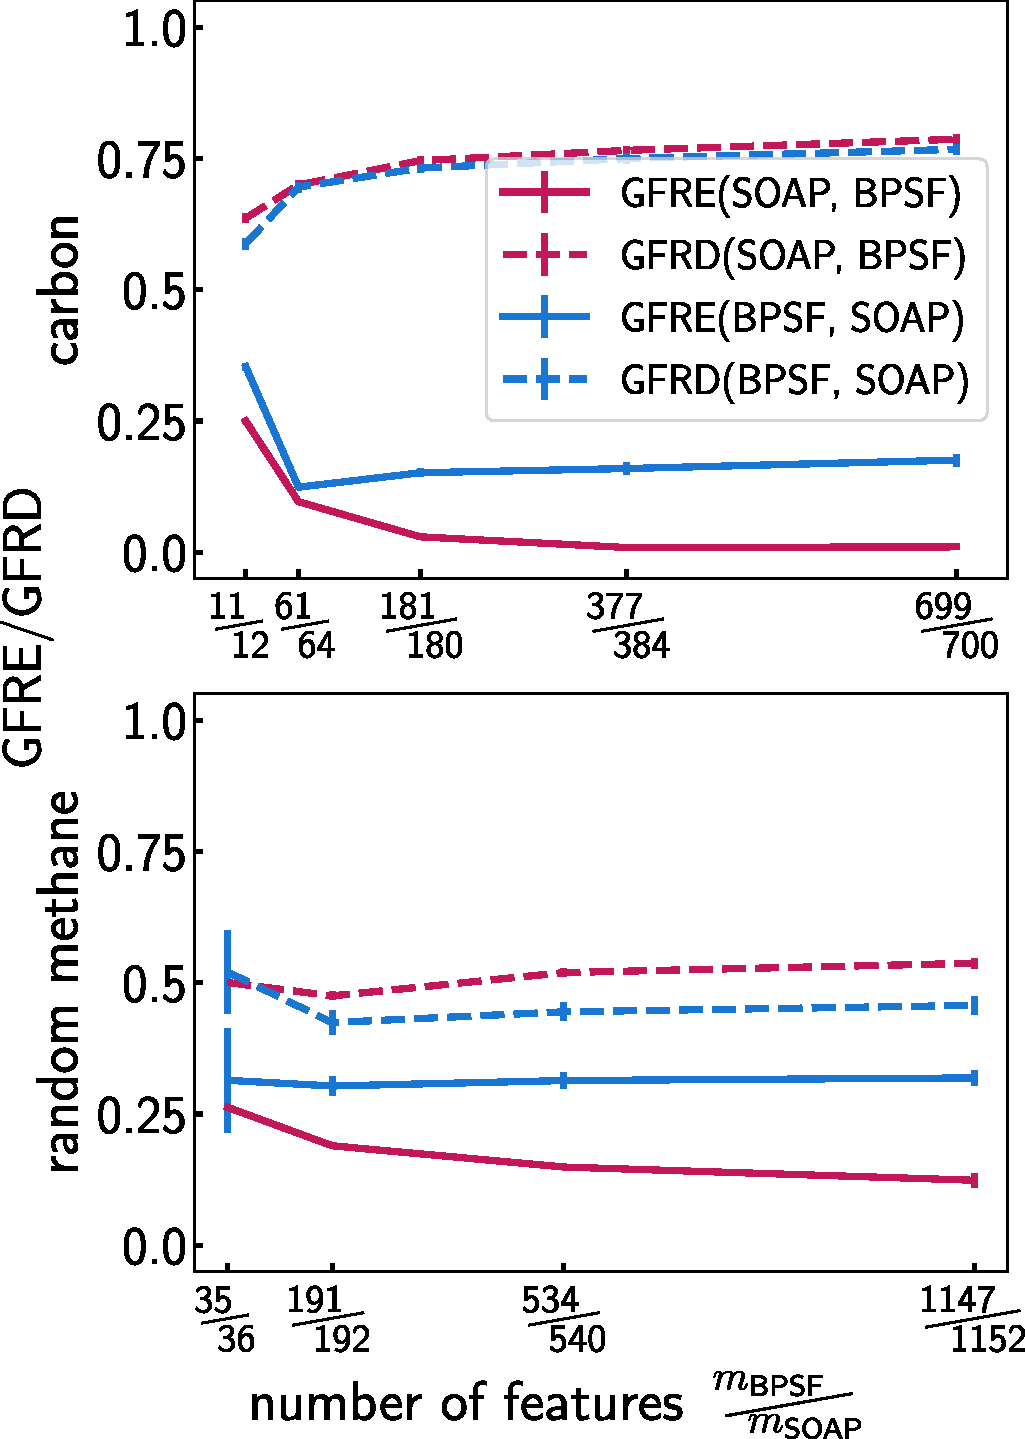
\includegraphics[width=0.45\linewidth]{fig/rof/symmetry_function_comparison-carbon_methane-updated_gfrd-inkscaped.pdf}
    \caption{Comparison of the GFRE and the GFRD between SOAP(GTO) and BPSF features with systematically-increasing sizes of the feature vectors. BPSF features are generated by varying over a grid the hyperparameters entering the definitions of $G^{(2)}$ and $G^{(3)}$, following Ref.~\citenum{imba+18jcp}. SOAP expansion truncation parameters $(\nmax,\lmax)$ are adjusted to approximately match the number of BPSF features.}
    \label{fig:soap_behler_parinello}
\end{figure}


\begin{figure}
    \centering
    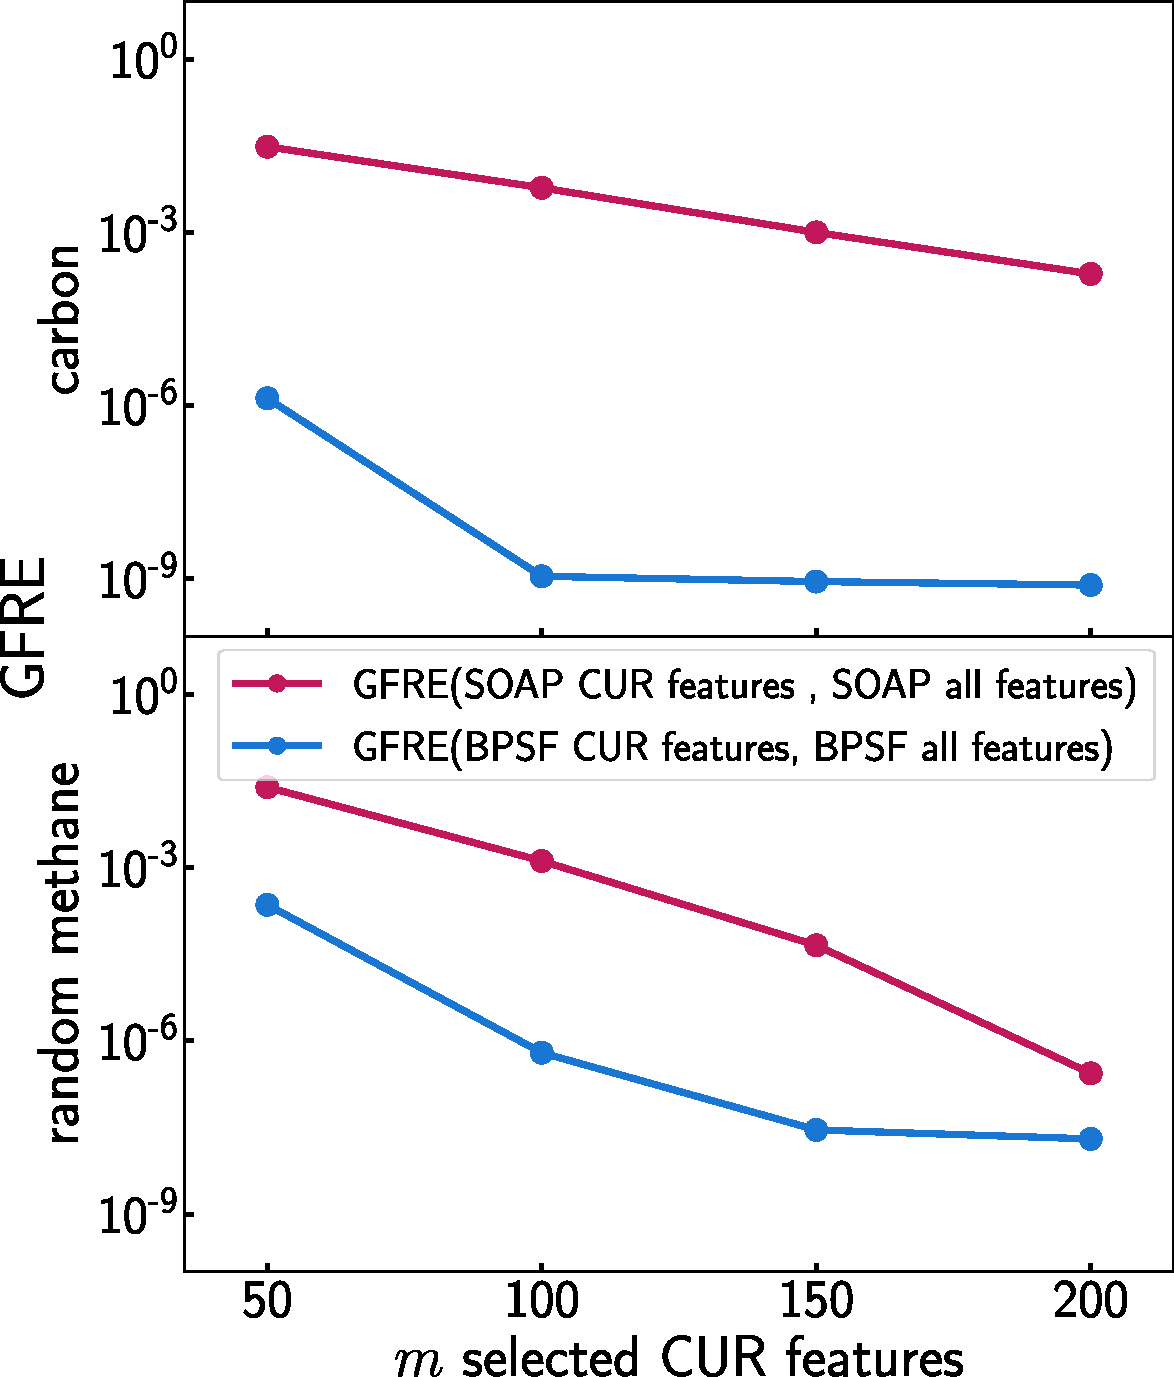
\includegraphics[width=0.45\linewidth]{fig/rof/feature_select_convergence_comparison-soap_bpsf-carbon_methane-inkscaped.pdf}
    \caption{Convergence of a CUR approximation of the full SOAP/BPSF feature vectors (the largest size considered in Figure~\ref{fig:soap_behler_parinello} )  with number of retained features.}
    \label{fig:soap_behler_parinello-convergence}
\end{figure}

\paragraph*{Behler-Parinello symmetry functions.}\,
BPSF can be seen as projections of the same, abstract symmetrized density features that underlies the construction of SOAP features.  While the latter representation is usually implemented using an orthogonal set of basis functions, BPSFs are non-orthogonal, and are usually chosen based on a careful analysis of the inter-atomic correlations that are relevant for a given system~\cite{behl11jcp,jose+12jcp,behl15ijqc}, or selected automatically out of a large pool of candidates~\cite{imba+18jcp}. 
Figure~\ref{fig:soap_behler_parinello} shows clearly that an orthogonal basis set provides a more effective strategy to converge a representation than the grid-based enumeration of the non-linear hyperparameters of non-orthogonal basis functions. GFRE(SOAP, BPSF) $<$ GFRE(BPSF, SOAP) for all feature set sizes and both data sets. As usual, we remark that zero reconstruction error does not imply equivalence for regression purpose: the GFRD remains very high even for the largest feature set sizes. 

Given that, in real scenarios, one would usually combine systematic enumeration of BPSF features with an automatic selection method\cite{imba+18jcp}, we also use the feature reconstruction framework to investigate the convergence of the automatic screening procedure, i.e. the error in reconstructing the full vector based on the first $m$ features chosen with a CUR decomposition-based procedure\cite{mahoney2009cur, imba+18jcp}.
Figure~\ref{fig:soap_behler_parinello-convergence} shows that a few dozens CUR-selected features allow to almost-perfectly reconstruct the full feature vector. The convergence is particularly fast for BPSF, where $m=50$ leads to a minuscule GFRE, indicating that the non-orthogonal features are highly redundant, and explaining the saturation in model performance that was observed in Ref.~\citenum{imba+18jcp}.

\begin{table*}[bthp]
\centering
\begin{tabular}{c|c|c|c||c|c}
\hline\hline
    $(n_\text{max},l_\text{max})$ & $m_\text{SOAP}$ & $t_\text{SOAP-GTO}$ / s&  $t_\text{SOAP-DVR}$ / s & $m_\text{BPSF}$ & $t_\text{BPSF}$ / s\\
    \hline
    (2,2) &  12 &  8.08 $\pm$ 0.30 &  7.95 $\pm$ 0.03 &  11 &   3.90 $\pm$ 0.14 \\ 
    (4,3) &  64 & 10.58 $\pm$ 0.03 &  9.57 $\pm$ 0.02 &  61 &  10.43 $\pm$ 0.22 \\
    (6,4) & 180 & 13.87 $\pm$ 0.03 & 11.87 $\pm$ 0.14 & 181 &  30.20 $\pm$ 0.41 \\
    (8,5) & 384 & 17.58 $\pm$ 0.05 & 14.50 $\pm$ 0.02 & 377 &  66.55 $\pm$ 0.55 \\
   (10,6) & 700 & 23.02 $\pm$ 0.04 & 18.57 $\pm$ 0.03 & 699 & 124.60 $\pm$ 0.78 \\
  \hline\hline
\end{tabular}
\caption{Timings in seconds for the evaluation of SOAP features using GTO ($t_\text{SOAP-GTO}$) and DVR ($t_\text{SOAP-DVR}$) as radial basis, and of BPSF $(t_\text{BPSF}$), using $r_c=4$\,\AA{}, on the entire carbon dataset. The SOAP discretization parameters are chosen to approximately match the number of features $m_\text{SOAP}$ and $m_\text{BPSF}$. 
The measurements have been conducted on a single  Intel(R) Xeon(R) CPU E3-1245 v6 @ 3.70GHz core, using librascal~\cite{LIBRASCAL} for SOAP features and n2p2~\cite{N2P2} for BPSF.}
\label{table:timings}
\end{table*}


\paragraph*{Computational cost}\,
In this work we focus on the comparison of  different kinds of features in terms of their information content, without commenting on the computational overhead associated with their evaluation, or the application of non-linear transformations.
Computational cost depends on implementation choices, and can be optimized for usage patterns that differ from those that we apply here. 
However, the effort associated with the evaluation of a model plays an important role in determining its ultimate usability. To provide some context for our experiments, we report in Table~\ref{table:timings} the timings for the evaluation of SOAP and BPSF features with the same parameters used in this Section. 
These timings show clearly that the computational savings afforded by the use of a DVR basis are not sufficient to offset the reduced information content with respect to the GTO basis.
When comparing BPSF and SOAP, the clearest difference is that the cost of evaluating the former scales linearly with the number of features, while the cost of evaluating SOAP features is sublinear since it is dominated by the calculation of the density expansion coefficients $c^i_{nlm}$ and is therefore sublinear with respect to the invariants. 
This difference in scaling is due to the different mechanism for evaluating 3-body terms, that scales quadratically with the number of neighbors for BPSF, and only linearly for SOAP, underscoring how a careful selection of the most relevant features is very important in the context of a BPSF framework. 

\begin{figure}
    \centering
    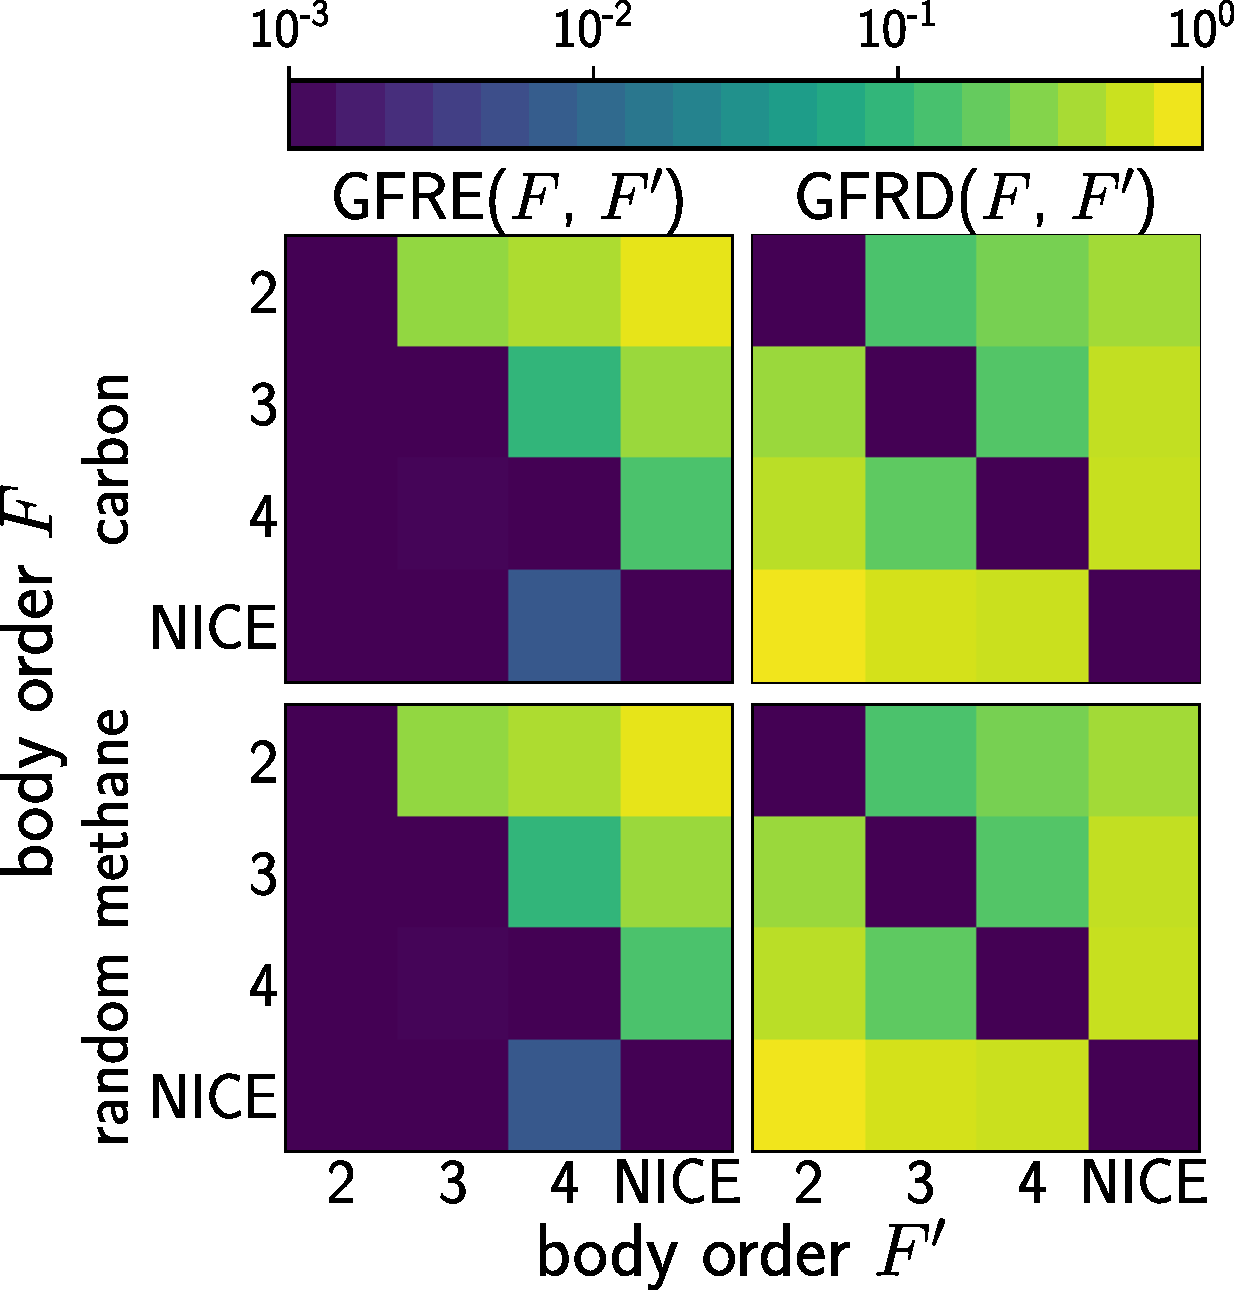
\includegraphics[width=0.5\linewidth]{fig/rof/body_order_comparison-gfrm-gto-methane_carbon-inkscaped.pdf}
    \caption{GFRE and GFRD body order comparison using GTO as radial basis function, $r_c= 4\,$\AA{}, $\sigma_G=0.5\,$\AA{} and $(n_\text{max},l_\text{max})=(6,4)$. NICE features were computed keeping the top 400 equivariant components at each level of the body-order iteration, and keeping invariant components up to $\nu=4$.  }
    \label{fig:soap-bodyorder}
\end{figure}


\subsection{ Body order feature truncation. }

The examples in Section~\ref{sub:hypers} demonstrate the impact of implementation details and hyperparameters choices on the information content of features that are all equivalent to a three-body correlation of the atom density. A more substantial issue is connected to the use of representations based on different $\nu$-body correlations of a decorated atom density, which is equivalent to the pair correlation function (2-body, $\nu=1$), to the SOAP power spectrum (3-body, $\nu=2$) or to the bispectrum (4-body, $\nu=3$).
Different orders incorporate conceptually distinct kinds of information: when used in linear regression, different density correlation orders correspond to a body-order expansion of the target property~\cite{shapeev2016moment,glie+18prb,will+19jcp,drau19prb,jinn+20jcp}, and the link between the convergence of the body-order expansion and the injectivity of the structure-feature map is an open problem, with known counter-examples showing that low values of $\nu$ are insufficient to achieve a complete representation of an atomic environment~\cite{pozd+20prl}.

\begin{figure}
    \centering
    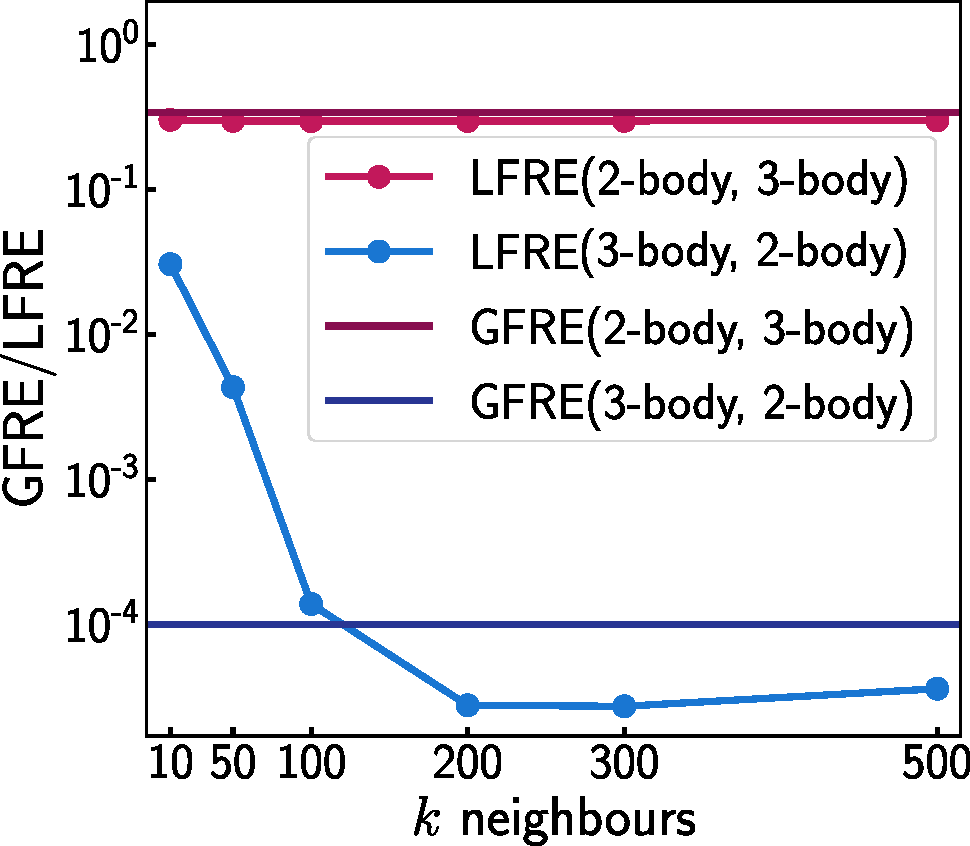
\includegraphics[width=0.5\linewidth]{fig/rof/lfre_convergence_comparison-methane-inkscaped-v3.pdf}
    \caption{Convergence of the LFRE between 2 and 3-body density correlation features (using GTOs as radial basis, $r_c= 4\,$\AA{}, $\sigma_G=0.5\,$\AA{} and $(n_\text{max},l_\text{max})=(6,4)$) with increasing number of neighbors.}
    \label{fig:soap-lfre-convergence}
\end{figure}

\begin{figure}
    \centering
    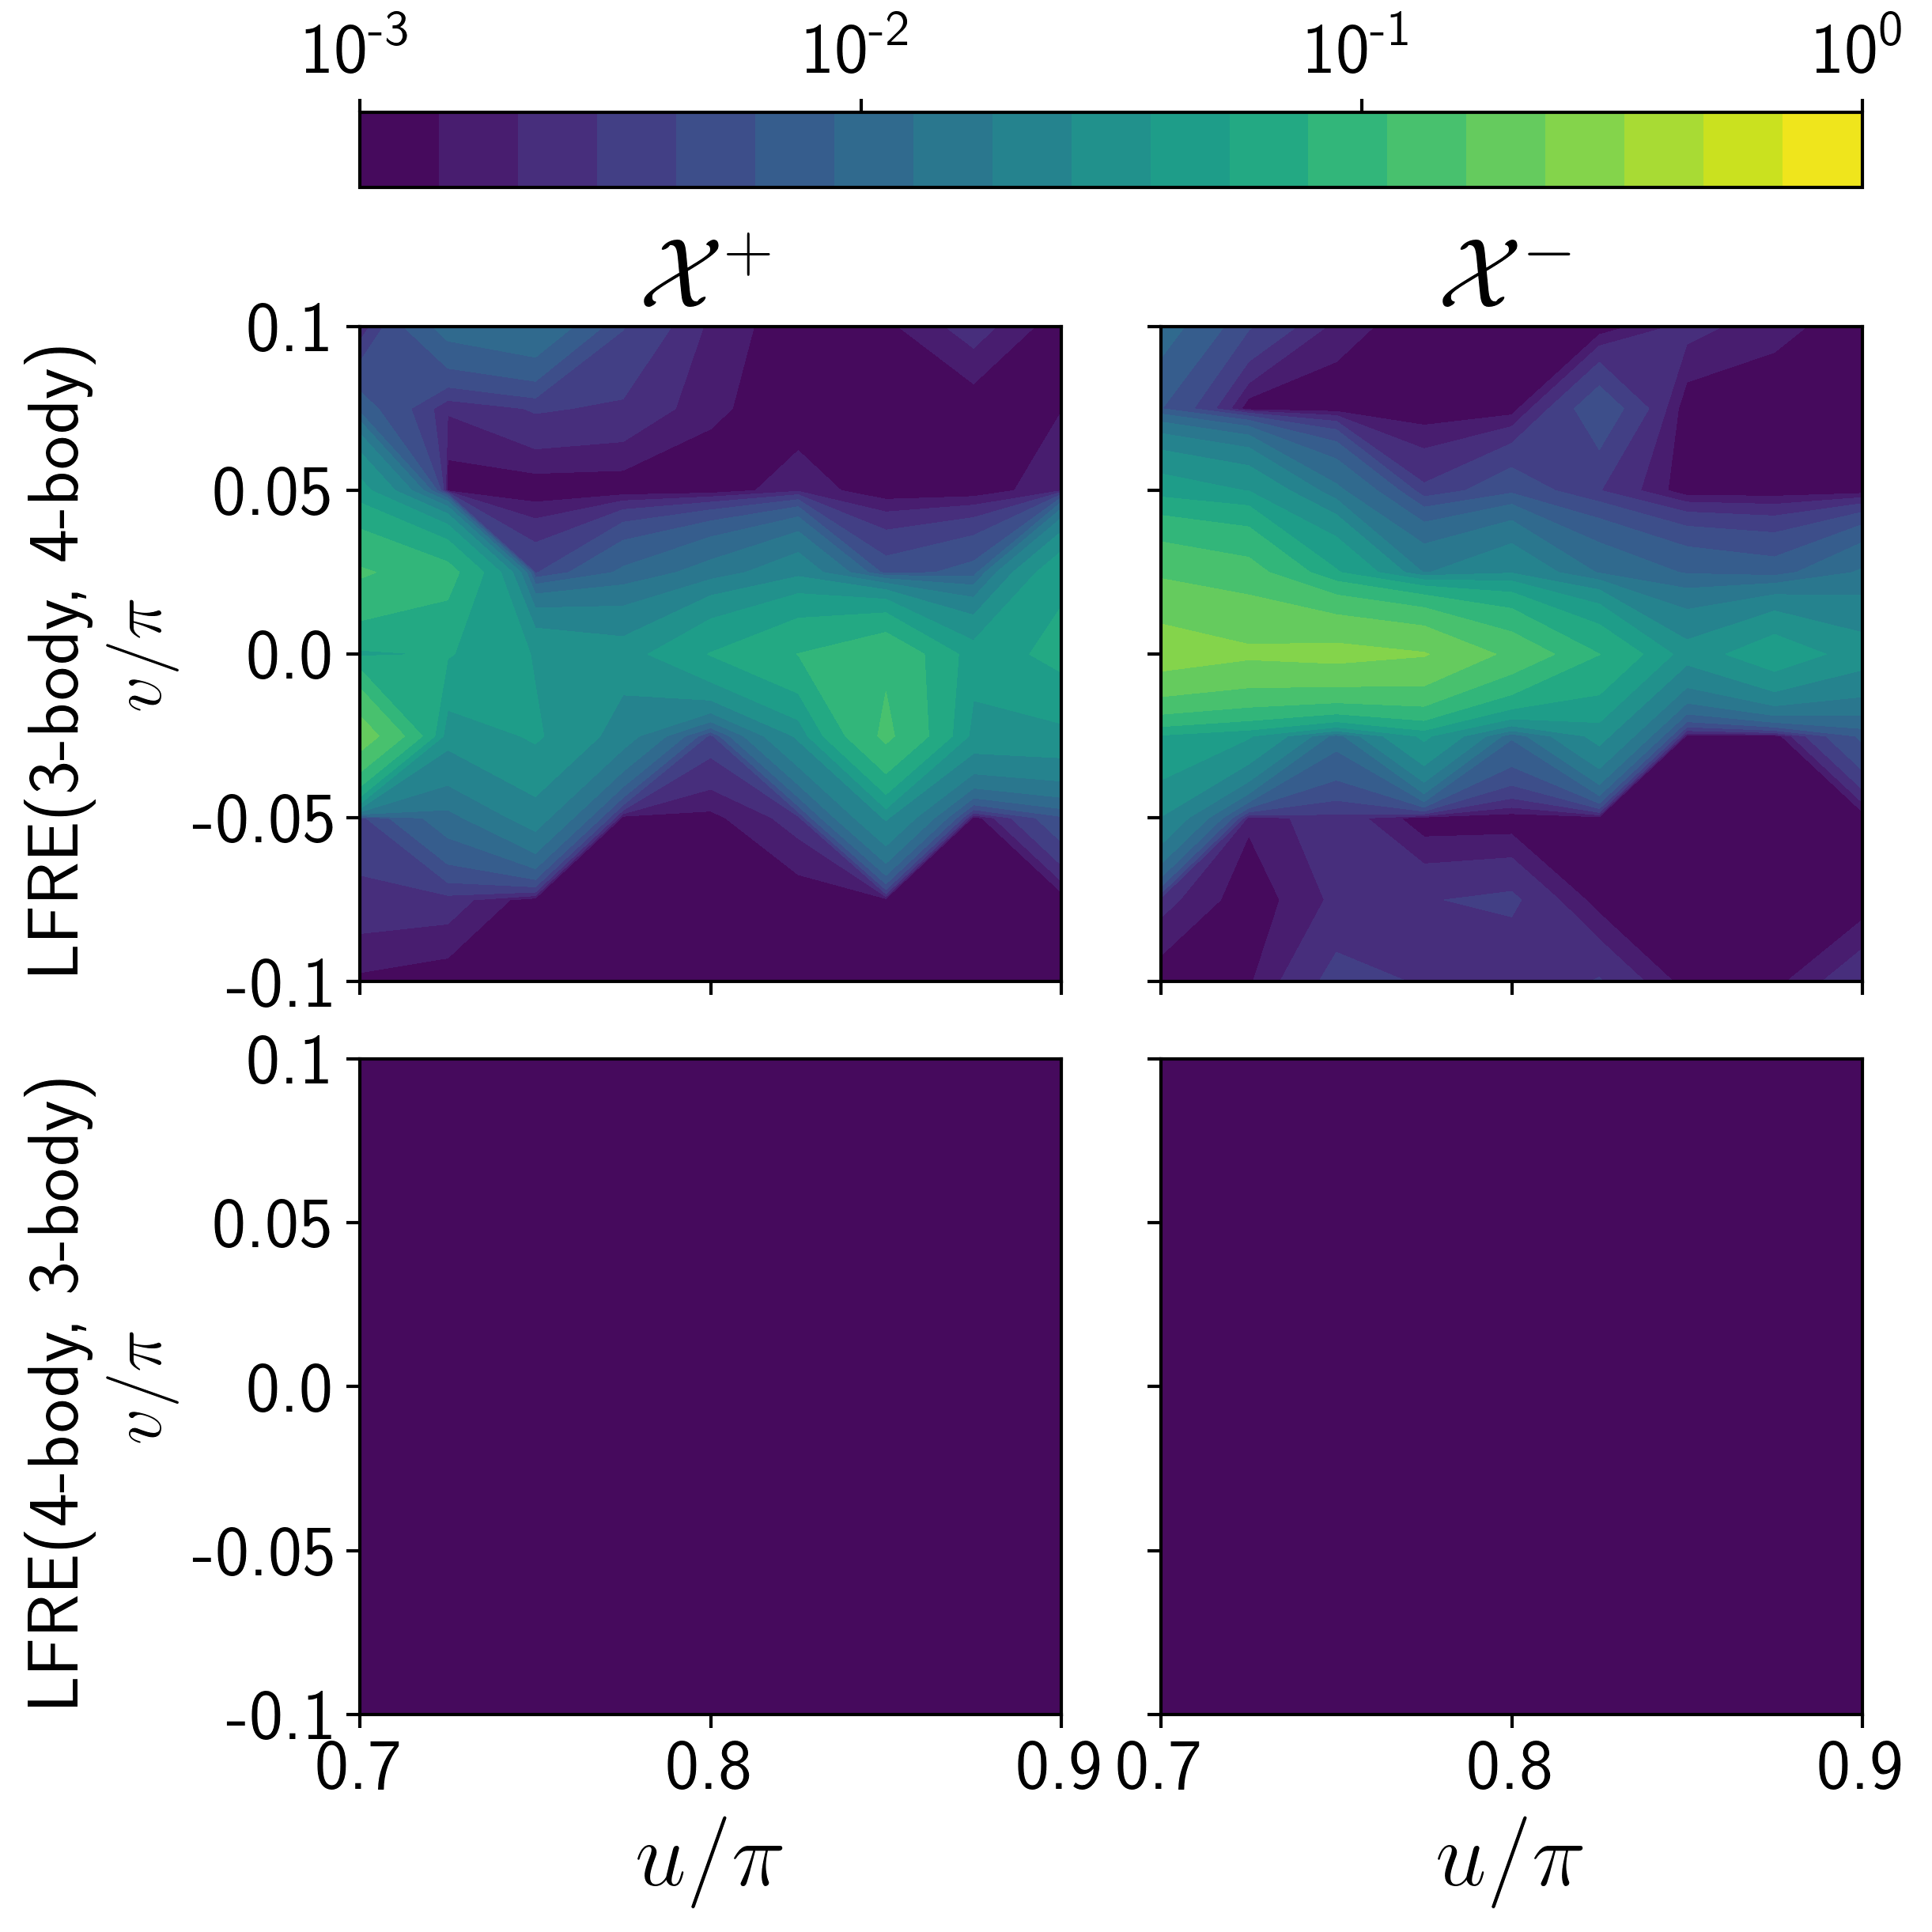
\includegraphics[scale=0.42]{fig/rof/lfre-body_order_comparison-nb_local_neighbours=15-degenerated_manifold.png}
\caption{Pointwise LFRE for the structures from the degenerate methane dataset as a function of the structural coordinates $(u,v)$ for $(\nmax,\lmax) = (6,4)$ and $k=15$ neighbors.}
    \label{fig:soap_degenerated_manifold_lfre}
\end{figure}

Figure~\ref{fig:soap-bodyorder} shows that high-order features cannot be recovered as linear functions of lower-order features, while an approximate (if not complete) reconstruction of lower-$\nu$ components based on high-$\nu$ components is possible. Reconstructing features of different order entails a large amount of distortion, with the GFRD approaching one in most cases. 
We also include in the comparison features obtained with the recently-developed $N$-body iterative contraction of equivariants (NICE) framework, that identifies the most important features for each $\nu$ value, and uses them to compute  $(\nu+1)$-order features~\cite{niga+20jcp}. Keeping 400 features for each body order is sufficient to achieve perfect reconstruction of 2 and 3-body features, but not for the 4-body (bispectrum) term, which cannot be reconstructed fully with 400 NICE features. Considering however that $\GFRE(\text{NICE},\nu=3)\ll \GFRE(\nu=3, \text{NICE})$, one can infer that the of information loss associated with truncating the body order expansion is more severe than when restricting the number of 4-body features. 

The comparison of features of different order can also be used to elucidate the role of the (non-)linearity of the mapping between feature spaces. Figure~\ref{fig:soap-lfre-convergence} compares global and local feature reconstruction errors between 2 and 3-body density correlation features, for the random $\ce{CH4}$ data set. In the case of the low-to-high body order reconstruction, the LFRE is only marginally lower than its global counterpart, indicating that the large $\GFRE(\nu=1,\nu=2)$ is a consequence of lower information content and not only of the linear nature of the map. The reverse case is also revealing: for small $k$-neighborhood sizes, $\LFRE(\nu=2,\nu=1)>\GFRE(\nu=2,\nu=1)$, because the small number of neighbors included in the model reduce the accuracy of the feature reconstruction map. When the number of neighbors approaches the intrinsic dimensionality of the $\nu=2$ features, instead, $\LFRE<\GFRE$ -- because the reconstruction is based on a locally-linear map that can approximate a non-linear relationship between features. As $k$ approaches the full train set size, the LFRE approaches the GFRE, as the locality of the mapping is lost. 

The LFRE also makes it possible to identify regions of phase space for which the construction of a mapping between feature spaces is difficult or impossible. 
Consider the case of the degenerate manifold discussed in Ref.~\citenum{pozd+20prl}. The dataset includes two sets of \ce{CH4} environments, and those parameterised by $v=0$ cannot be distinguished from each other using 3-body ($\nu=2$) features.
Figure~\ref{fig:soap_degenerated_manifold_lfre} shows the LFRE for each point along the two manifolds. When trying to reconstruct 3-body features using as inputs 4-body features (that take different values for the two manifolds) the LFRE is essentially zero. When using the 3-body features as inputs, instead, one observes a very large error for points along the degenerate line, while points that are farther along the manifold can be reconstructed well. This example demonstrates the use of the LFRE to identify regions of feature space for which a simple, low-body-order representation is insufficient to fully characterize the structure of an environment, and can be used as a more stringent, explicit test of the presence of degeneracies than the comparison of pointwise distances discussed in Ref.~\citenum{pozd+20prl}. 

\subsection{Kernel-induced feature spaces}

With the exception of the trivial, scalar-product form, a kernel introduces a non-linear transformation of the feature space, potentially allowing to obtain more accurate regression models. 
A crucial aspect of kernel methods is the fact that this non-linear transformation gives rise to a linear feature space that is defined by the combination of the kernel and the training samples -- or the active samples in the case of sparse kernel methods.
We can then use our feature-space reconstruction framework to compare quantitatively the linear feature space with the kernel-induced features. We do so using a radial basis function kernel, varying the $\gamma$ parameter. In the $\gamma\rightarrow 0$ limit the RBF kernel becomes roughly linear, and the non-linearity increases with growing $\gamma$. The use of standardized input features means that $\gamma$ is effectively unitless, and also standardize the kernel-induced features. 
To reduce noise, given that the kernel matrices are often very ill-conditioned, we only retain the RKHS features that are associated with the largest eigenvalues, preserving those that together contribute to approximately 99\%{} of the variance.
Figures~\ref{fig:rbf-density} and~\ref{fig:rbf-bo-promote} plot the GFRE for the mapping of linear and RBF features computed for 2 and 3-body density correlations. The non-linear nature of the transformation is apparent in the increase in the GFRE(linear,RBF) for larger values of $\gamma$, for both $\nu=1$ and $\nu=2$. The transformation is not entirely lossless, as evidenced by the fact that the reverse GFRE is also non-zero. The GFRE(RBF, linear) becomes particularly large for very large values of the $\gamma$ parameter. This can be understood from the fact that the decay of the kernel becomes very sharp, and it only provides information about the nearest neighbors of each point -- effectively leading to an ill-conditoned regression problem as we show in more detail below. 

\begin{figure}
    \centering
    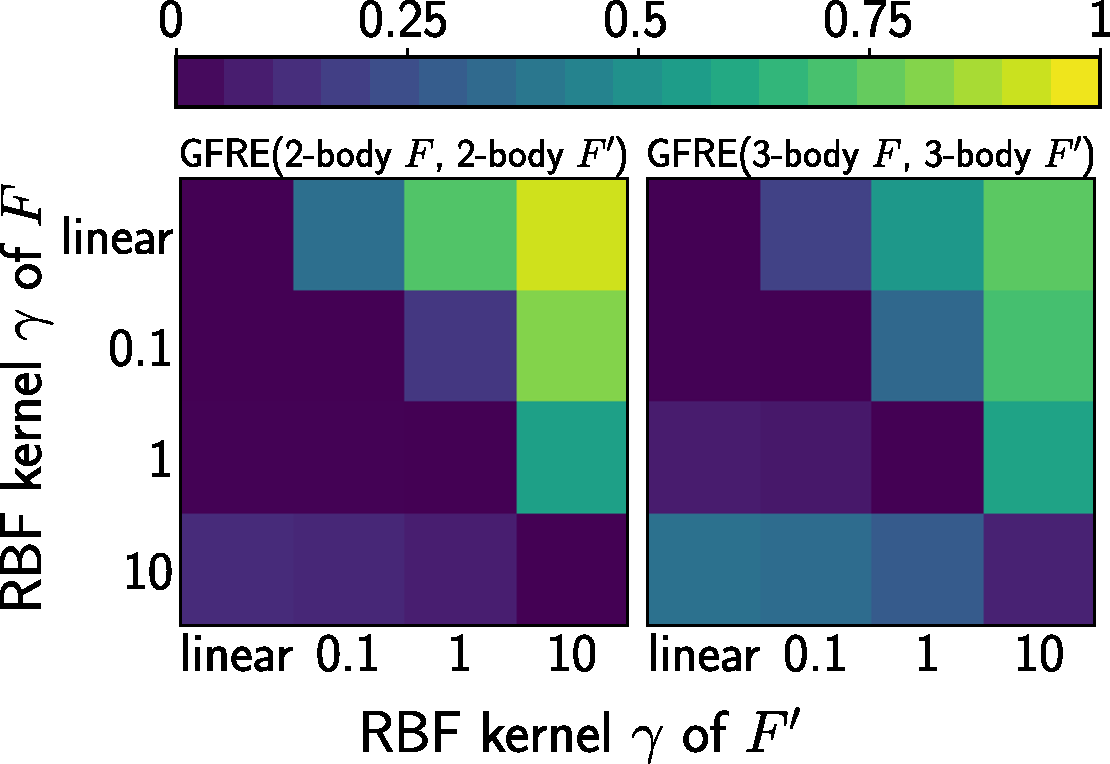
\includegraphics[width=0.7\linewidth]{fig/rof/body_order_comparison-gfrm-rs_ps-methane-inkscaped-v3-fixed_rkhs_features.pdf}
    \caption{GFRE on the random methane dataset for interconverting the linear 2-body (left) and 3-body (right) feature spaces with those induced by a RBF kernel with different inverse  kernel width $\gamma$.}
    \label{fig:rbf-density}
\end{figure}

\begin{figure}
    \centering
    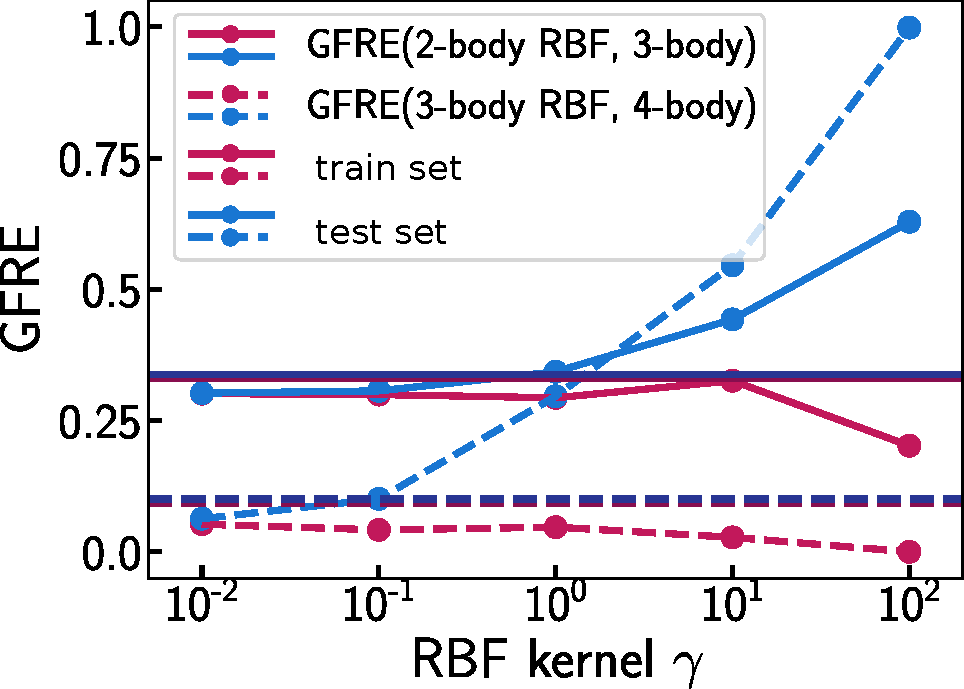
\includegraphics[width=0.6\linewidth]{fig/rof/gamma_plot-methane-inkscaped-ver3-fixed_rkhs_features.pdf}
    \caption{GFRE on the random methane dataset curves as a function of the $\gamma$ hyperparameter of $k^{\text{RBF}}_E$.
    Values for train and test sets are plotted separately. The horizontal lines correspond to the GFRE of the linear features.}
    \label{fig:rbf-bo-promote}
\end{figure}

\begin{figure*}
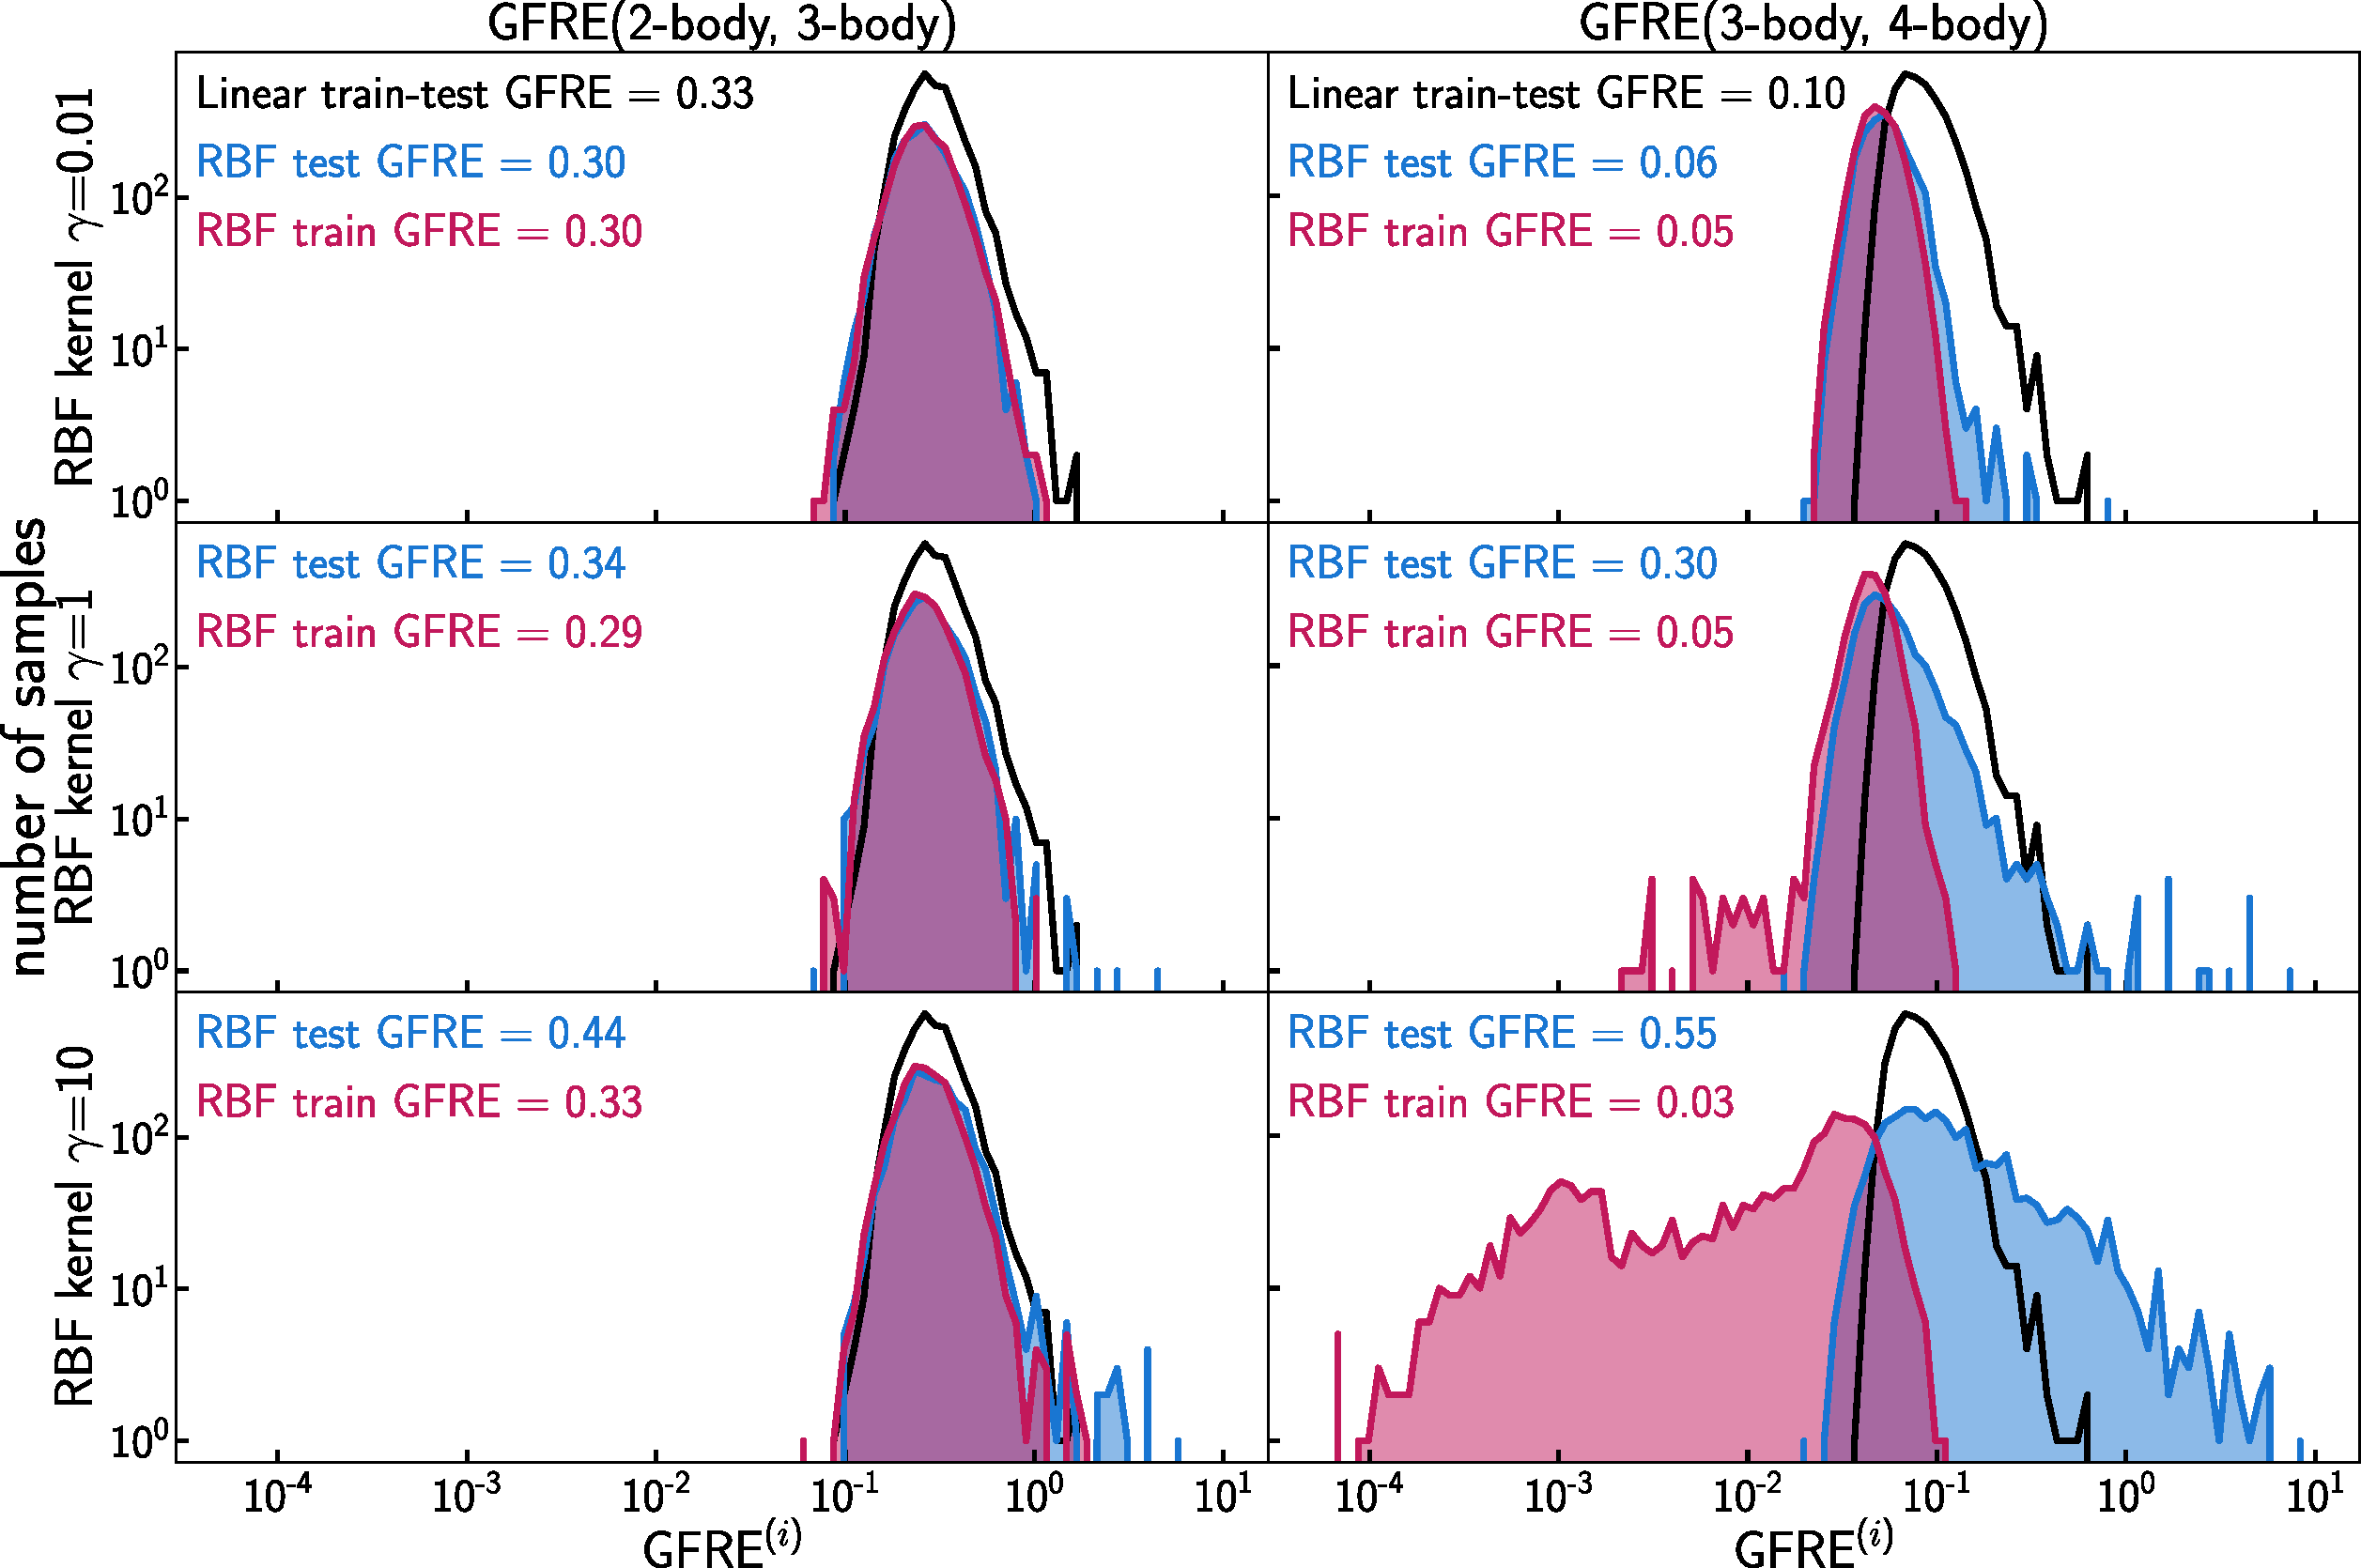
\includegraphics[width=0.9\linewidth]{fig/rof/ffre_kernel_train_test_hist-rs_ps-rbf-methane-inkscaped-ver2_fixed_rkhs_features.pdf}
\caption{Histograms of the pointwise reconstruction error for $2\rightarrow 3$ (left) and $3\rightarrow 4$ (right) body order features, using a RBF kernel with different values of $\gamma$ (top to bottom, $\gamma=$ 0.01, 1.0, 10) to reconstruct the higher body order features. Red curves refer to the train set points, blue curves to the test set, and the black line correspond to the linear train-test set GFRE, that serves as a reference.}
    \label{fig:rbf-body-hists}
\end{figure*}


Having assessed the impact of non-linear kernel features on a single body order representation, we can then investigate whether a non-linear transformation helps inferring high-body order correlations from low-body-order features.
This is relevant because the use of non-linear kernels has been proposed~\cite{glie+18prb} (and used in practice for a long time~\cite{bart+10prl,bart+13prb}) as a strategy to describe many-body effects on atomistic properties.
We compute the GFRE for promoting $\nu=1$ (2-body) to $\nu=2$ (3-body) and $\nu=2$ to $\nu=3$ features for different values of the RBF kernel $\gamma$. 
In Figure~\ref{fig:rbf-bo-promote} we show these curves for both the usual GFRE definition (that involves a separate test set) and for a prediction carried out on the train set. 
These results show that while a non-linear kernel does allow a low-body-order model to discern higher body-order features, it does so in a poorly transferable way: high-$\gamma$ models show much reduced GFRE for train-set predictions, but lead to a degradation in the feature reconstruction for the test set. 
Only low-$\gamma$ models show a small improvement in the test-set GFRE compared to an entirely linear mapping. In this regime, the RBF kernel is dominated by the low-exponent components of the Gaussian expansion, vindicating the choice of low-order polynomial kernels, that are used in most of the published SOAP-based potentials. 
A better understanding of the effect of a non-linear feature space transformation can be obtained by analyzing the distribution of reconstruction errors for individual samples
\begin{equation}
\GFRE^{(i)}(\CF,\CF^{\prime}) = \norm{\bx^{\prime}_i - \bx_i\bP{\CF}{\CF^{\prime}}}. 
\label{eq:pointwise_GFRE}
\end{equation}
The histograms for this ``pointwise $\GFRE$`` (Figure~\ref{fig:rbf-body-hists}) show that increasing the non-linearity of the kernel does indeed allow to reconstruct more accurately a fraction of both the test and the train set. When extrapolating the mapping to points that have not been seen before, however, there is an increasingly large fraction of outliers for which the reconstruction is catastrophically poor.

The pointwise errors are also revealing of the different nature of the $\nu=1\rightarrow \nu=2$ and $\nu=2\rightarrow \nu=3$ cases.
In the former case, the clear lack of information in the 2-body descriptor makes it impossible, even for a highly non-linear kernel, to obtain an accurate reconstruction of higher body-order features.
In the latter case, instead, the train set reconstruction become nearly perfect with large $\gamma$ -- indicating that despite the existence of degenerate manifolds of configurations~\cite{pozd+20prl} it is possible to reconstruct $4$-body features using only $3$-body inputs, for  structures that are not exactly on the degenerate manifold.
However, the increasingly large tail of very high test-set GFRE samples suggests that this mapping is not smooth, and rather unstable. When building a regression model for a property that depends strongly on 4-body terms, this instability may translate into poor extrapolative power for a non-linear model based on 3-body features.

\begin{figure*}
    \centering
    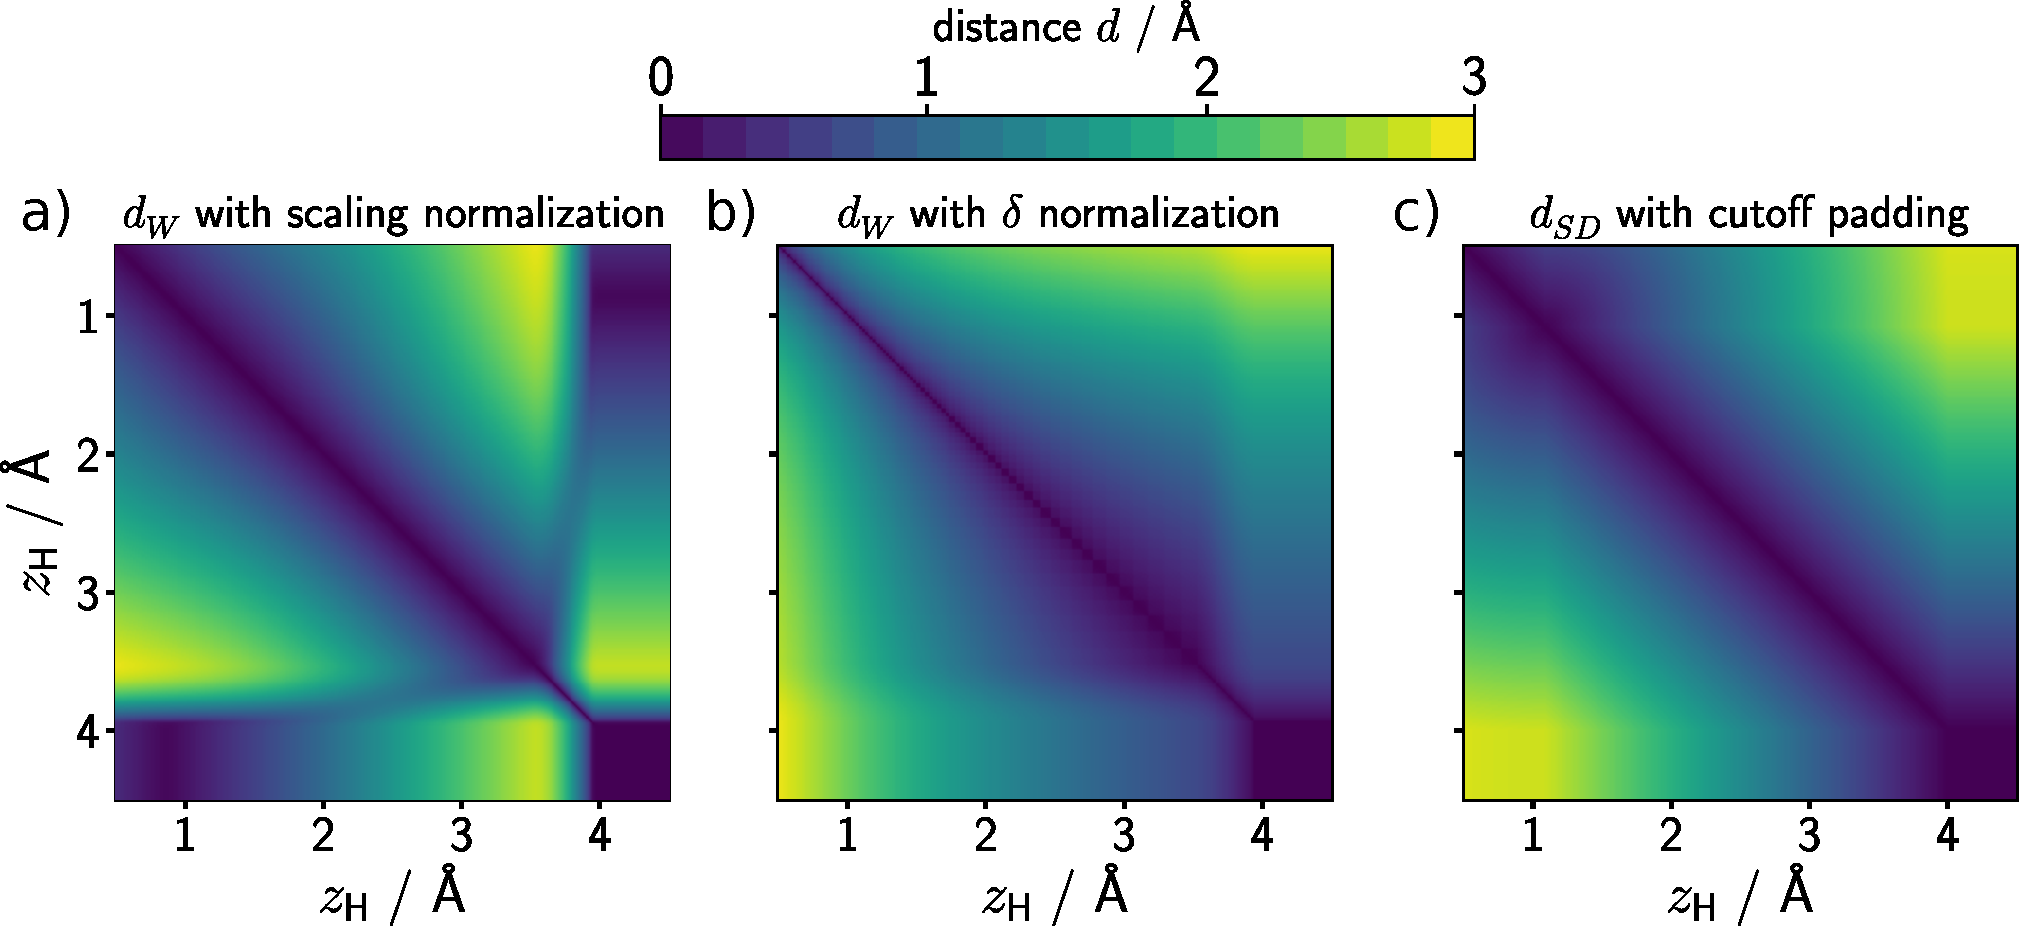
\includegraphics[width=0.77\linewidth]{fig/rof/displace_wasserstein_distance_plots.pdf}
    \caption{Distance between two \emph{displaced methane} configurations with different values of $\zh$, computed using a Wasserstein distance using (a) scaling normalization; (b) cutoff $\delta$ normalization; (c) Euclidean distance between sorted interatomic distance vectors.}
    \label{fig:wasserstein-distances}
\end{figure*}

\begin{figure}
  \centering
  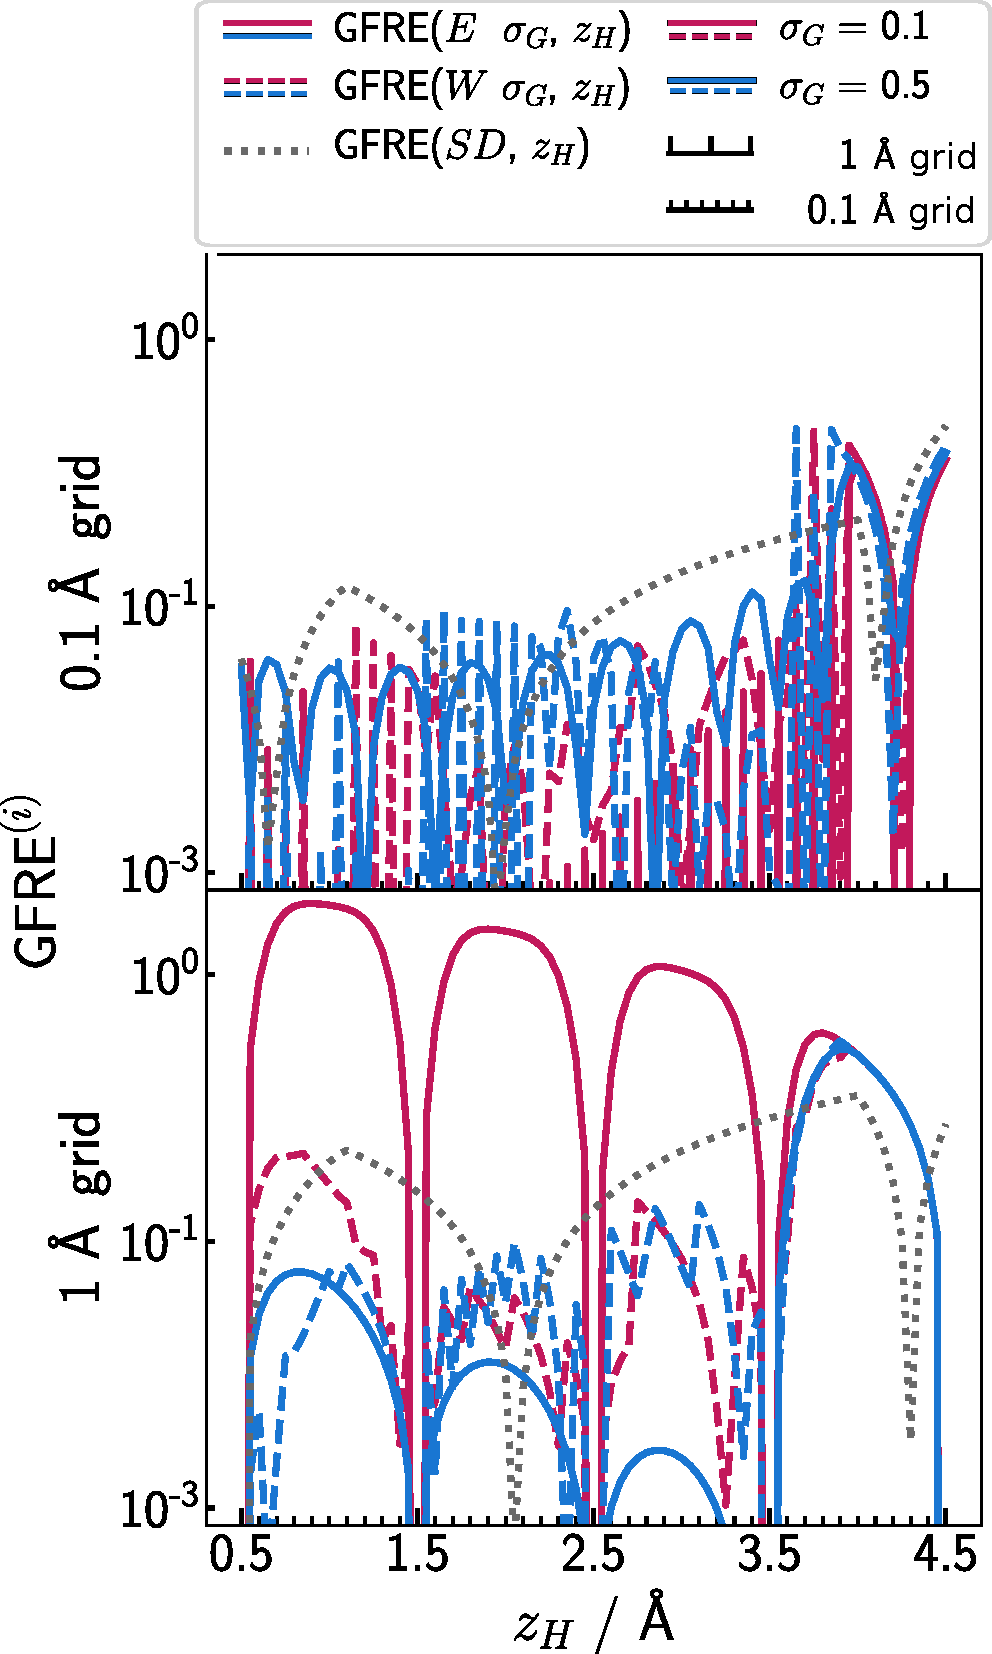
\includegraphics[width=0.45\linewidth]{fig/rof/test_errors-displaced_methane-2x1-inkscaped-ver2.pdf}
\caption{
Errors when reproducing the atomic displacement $\zh$ for a fine (top) and coarse (bottom) grid of training points, and different Gaussian $\sigmag$ and metrics. A constant regularization that discards singular values smaller than \revadd{$10^{-3}$} has been applied to all pointwise GFRE calculations.}
\label{fig:wasserstein-grid}
\end{figure}

\subsection{Wasserstein metric}
As an example of the transformation induced by a non-Euclidean metric we consider the effect of using a Wasserstein distance to compare $\nu=1$ density correlation features. 
The Wasserstein distance is defined as the minimum  ``work`` that is needed to transform one probability distribution into another -- with the work defined as the amount of probability density multiplied by the extent of the displacement~\cite{vall74siam,cohe-guib97report,cutu07proc}.
The EMD has been used to define a ``regularized entropy match`` kernel to combine local features into a comparison between structures~\cite{de+16pccp}, to obtain permutation-invariant kernels based on Coulomb matrices~\cite{cayl+20mlst}.
Here we use the Wasserstein distance to compare two-body ($\nu=1$) features, that can be expressed on a real-space basis and take the form of one-dimensional probability distributions. 
% MC  this looks like an entirely general definition >> More formally, for an atomic environment with cutoff $r_c$, we can define the $\nu$-body 

The formal definition of the Wasserstein distance of order 2 between two probability distributions $p(r)$ and $p^{\prime}(r)$ defined on a domain $M$ reads
\begin{equation}
W(p,p^{\prime})^2 = \hspace{-1em}\inf_{\gamma\in\Gamma (p,p^{\prime})} \int_{M\times M}\hspace{-0.5em}d(r,r^{\prime})^2\,\mathrm{d}\gamma(r,r^{\prime}),
%W_2(p_{\mathcal{X}_i},p_{\mathcal{X}_j})^2 = \hspace{-1em}\inf_{\gamma\in\Gamma (p_{\mathcal{X}_i},p_{\mathcal{X}_j})} \int_{M\times M}\hspace{-0.5em}d(r,r^{\prime})^2\,\mathrm{d}\gamma(r,r^{\prime}),
%
%W_2(p_{\mathcal{X}^{(\nu)}_i},p_{\mathcal{X}^{(\nu)}_j})^2 = \hspace{-1em}\inf_{\gamma\in\Gamma (p_{\mathcal{X}_i^{(\nu)}},p_{\mathcal{X}_j^{(\nu)}})} \int_{M^{\nu}\times M^{\nu}}\hspace{-2.5em}d(r,r^{\prime})^2\,\mathrm{d}\gamma(r,r^{\prime}), Adding many body order makes it too cluttered
%\mathcal{X}_i = \int_{M^{\nu}} \gamma(x,x^{\prime})\,\mathrm{d}x I would not write this out because \mathcal{X} is not a probability distribution without any transformation, this way we keep the definition of \Gamma open
\end{equation}
where $\Gamma(p,p^{\prime})$ is the set of all joint distributions with marginals $p$ and $p^{\prime}$.
For 1-dimensional distributions, $W(p,p^{\prime})$ can be expressed as the 2-norm of the difference between the associated inverse cumulative distribution function (ICDF) $P^{-1}$ of two environments,
$W(p,p^{\prime})^2=\int_0^1  \left|P^{-1}(s) -{P^{\prime}}^{-1}(s)\right|^2\D{s}$, with $P(r)=\int_0^r p(r)\D{r}$ 

In order to express the symmetrized 2-body correlation function as a probability density, we first write it on a real-space basis $r$, and evaluate it on 200 Gaussian quadrature points, that we also use to evaluate the CDF and its inverse. 
We then proceed to normalize it, so that it can be interpreted as a probability density.
We estimate the integral of the distribution (that effectively counts the number of atoms within the cutoff distance) 
\begin{equation}
Z_i = \int_0^{r_c} \overline{\rho_i^{\otimes 1}}(r)\,\mathrm{d}r,
\end{equation}
and the maximum value of the integral over the entire dataset $Z_\CD$.
A simple scaling of the correlation function 
\begin{equation}
p_i^{\text{s}}(r) = \frac1{Z_i} \overline{\rho_i^{\otimes 1}}(r)\label{eq:wass-pis}
\end{equation}
distorts the comparison between environments with different numbers of atoms.
To see how, we use the \emph{displaced methane} dataset, in which three atoms in a \ce{CH4} molecule are held fixed in the ideal tetrahedral geometry, at a distance of 1\AA{} from the carbon centre. The fourth atom, aligned along the $z$ axis, is displaced along it, so that each configuration is parameterised by a single coordinate $\zh$.
Figure~\ref{fig:wasserstein-distances}(a) shows the distance computed between pairs of configurations with different $\zh$,  demonstrating the problem with the renormalized probability~\eqref{eq:wass-pis}: $p^{\text{s}}$ loses information on the total number of atoms within the cutoff, and so once the tagged atom moves beyond $r_\text{c}$ the remaining \ce{CH3} environment becomes indistinguishable from an ideal \ce{CH4} geometry. 

One can obtain a more physical behavior when atoms enter and leave the cutoff by introducing a $\delta$-like ``sink`` at the cutoff distance, defining
\begin{equation}
p^{\delta}_i(r) = \frac{1}{Z_\CD}\left[\overline{\rho_i^{\otimes 1}}(r) + (Z_\CD-Z_i)\delta(r-r_c)\right].
\end{equation}
Figure~\ref{fig:wasserstein-distances}b shows that with this choice the Wasserstein metric between $p_i^\delta(r)$ reflects the distance between the moving atoms. With this normalization, in fact, the Wasserstein metric corresponds to a smooth version of the Euclidean metric computed between vectors of sorted interatomic distances~\cite{will+19jcp}, shown in Figure~\ref{fig:wasserstein-distances}c. 
The distortions that can be seen in the comparison between Figure~\ref{fig:wasserstein-distances}b,c are a consequence of the Gaussian smearing, the smooth cutoff function, and the $\SOthree$ integration that modulates the contribution to $\overline{\rho_i^{\otimes 1}}(r)$ coming from atoms at different distances.

Having defined a meaningful normalization and a probabilistic interpretation of the radial density correlation features, we can investigate how the feature space induced by a Wasserstein metric relates to that induced by an Euclidean distance. 
Figure~\ref{fig:wasserstein-grid} shows the error in the reconstruction of $\zh$ for the \emph{displaced methane} dataset when restricting the training set to 0.05\AA{} and 1.0\AA{} spaced grids.
Using a Euclidean distance with a sharp $\sigmag$ leads to a highly non-linear mapping between the displacement coordinate and feature space, and a linear model cannot interpolate accurately between the points of a sparse grid. 
A Wasserstein metric, on the other hand, measures the minimal distortion needed to transform one structure into another, and so provides a much more natural interpolation along $\zh$, which is robust even with a sharp density and large spacing between training samples. 
It is worth stressing that the sorted distance metric -- which effectively corresponds to the $\delta$ density limit of the Wasserstein metric -- performs rather poorly, and cannot even reproduce the training points.
This is because the mapping between feature space and $\zh$ is not exactly linear, changing slope when $\zh$ crosses 1\AA{} (because the sorting of the vector changes)  and 4\AA{} (because one atom exits the cutoff). The sorted-distances feature space does not have sufficient flexibility to regress this piecewise linear map, as opposed to its smooth Wasserstein counterpart.

\begin{figure}
  \centering
  \includegraphics[width=0.6\linewidth]{fig/rof/distance_comparison-delta_wasserstein-carbon-inkscaped.pdf}
\caption{Comparison of GFRE and GFRD for the \emph{carbon} dataset, using sharp ($\sigmag=0.1$\AA{}) and smooth ($\sigmag=0.5$\AA{}) radial SOAP features, as well as Euclidean (E) and Wasserstein (W) metrics.}
\label{fig:wasserstein-carbon}
\end{figure}

Having rationalized the behavior of the Wasserstein metric for a toy model, we can test how it compares to the conventional Euclidean metric on a more realistic data set. We consider in particular the AIRSS \emph{carbon} data set, and compare different levels of density smearing as well as Euclidean and Wasserstein metrics. 
Figure~\ref{fig:wasserstein-carbon} paints a rather nuanced picture of the relationship between the linear and the Wasserstein-induced feature spaces. 
The GFRE is non-zero in both directions, meaning that (in a linear sense) Wassertein and Euclidean features provide complementary types of information. 
Smearing of the density has a small effect on the Wasserstein metric, so that both $\GFRE(W(\sigmag=0.1\text{\AA}),W(\sigmag=0.5\text{\AA}))$ and $\GFRD(W(\sigmag=0.1\text{\AA}),W(\sigmag=0.5\text{\AA}))$ are small, whereas for Euclidean features -- as observed in Section~\ref{sub:hypers} -- changing $\sigmag$ induces small information loss, but a large distortion of feature space. 
Overall, there is no sign of the pathological behavior seen in Figure~\ref{fig:wasserstein-grid}, which is an indication that (at least for 2-body features) the \emph{carbon} dataset is sufficiently dense, and that the better interpolative behavior of the EMD does not lead to a more informative feature space. 


%where $Z_\mathcal{D}$ is the maximum $Z_i$ value of a dataset $\mathcal{D}$.The iCDF has been approximated from the CDF \begin{equation}    F_i(r) = \int_0^{r}p_i(r^{\prime})\,\mathrm{d}r^{\prime}\quad\text{(CDF)},\end{equation} by a linear interpolation using $200$ Gaussian quadrature points of the CDF in the range of $[0,r_c]$. Likewise, for the distance comparison $200$ Gaussian quadrature points of the interpolated iCDF were used to approximate the Wasserstein distance and the same amount of points of the unnormalized density $p_i$ were used for the Euclidean distance.


\section{Conclusion}

Applications of machine learning to atomistic modelling suggest that the featurization that is chosen to represent a molecule or material can be equally or more important than the choice of regression scheme~\cite{fabe+17jctc}. 
This has led to the proliferation of approaches to build descriptors, that often differ from each other only in implementation details. 
The framework we introduce in this work enables a comparison of alternative choices of representations that does not depend on the target property, and makes it possible to determine objectively which of two features contains more information -- based on a feature-space reconstruction error --  and how much distortion is present in the way they describe the information that is common between the pair -- based on a measure of feature-space distortion. 
Even though the framework is linear in nature, it can be generalized to account for non-linear relationships between feature spaces, either by using kernel-induced features, or by decomposing the feature comparison problem into a collection of local mappings. 

Using this framework we demonstrate that the choice of basis set can affect substantially the convergence of SOAP features, and that for instance  Gaussian type orbitals are more stable in the limit of small density smearing than the discrete variable representation basis. 
In practice the convergence of the representation with the number of basis functions should be considered together with the computational cost of the basis. The analytical expression for GTOs involve special functions that are usually harder to evaluate than those that appear for a DVR basis. This overhead, however, is not sufficient to compensate for the reduced information content, and can be avoided altogether by using a spline approximation for the special functions. In general, computational cost depends substantially on the details of the implementation, and should be assessed in an end-to-end manner as a function of the specific use case.
We also show quantitatively that a systematic orthogonal basis is much more effective in describing the atom density than the heuristic symmetry functions of the Behler-Parrinello kind -- notwithstanding the considerable success that the latter approach has had in the construction of neural-network-based interatomic potentials~\cite{behl16jcp}. 

A more systematic difference between atomistic machine-learning frameworks arises from the choice of the order of inter-atomic correlations that underlies the representation. 
We show that atom density correlation features of high body order make it possible to approximately reconstruct low-body order features, while the opposite is not true. Even when using a non-linear (or locally-linear) mapping, reconstructing 3-body features from 2-body information is virtually impossible.
The 3-to-4-body mapping is more subtle: an overall reconstruction based on a linear model is not possible, but a local mapping works well, provided that the structures are far from the manifold of structures for which the 3-body description is not injective.
The associated transformation, however, is highly non-linear, and a kernel model that can reconstruct 4-body features shows poor transferability outside of the training set, which hints at similar shortcomings whenever one wanted to use it to learn a property that depends strongly on 4-body correlations. 
Even though an overall linear reconstruction is not possible, the $\nu$-to-$(\nu+1)$-body mapping error decreases with increasing $\nu$, indicating that less information is added with higher body-orders.  
This is consistent with the satisfactory results that have been obtained in the regression of atomistic properties using only 3-body information~\cite{glie+18prb, paru+18ncomm}, even though the fundamental incompleteness of 3-body features has been shown to have implications for the asymptotic learning performance~\cite{pozd+20prl}. 
An analysis based on the GFRE might help determine the high-order correlations that provide the highest amount of information, and combined with an iterative scheme to evaluate the corresponding features~\cite{niga+20jcp} provide a strategy to increase model accuracy with an affordable computational effort.

We also investigate the effect of changing the metric used to compare features, by juxtaposing the Euclidean distance (that is induced by a linear description of the feature space) with a Wasserstein metric, that can be applied to the comparison of $n$-body correlation features when expressed as real-space distributions. We find that -- with an appropriate normalization -- the Wasserstein distance can be seen as a proxy of the minimal amount of distortion needed to transform an environment into another, and that this behavior induces smooth interpolation between sparse reference points, contrary to what is observed for the Euclidean distance. 
However, both an aggressive smearing of the atom density, and the use of a more realistic data set cure the pathological behavior of the linear featurization, so that the Wasserstein metric should not be regarded as superior to the Euclidean one, but complementary. Generalizing the Wasserstein metric to higher body-order correlations, which induce a higher-dimensional feature space that is more likely to be sparsely populated, would be an interesting further research direction.
% might mention discontinuity

It further is not clear how the change to the Wasserstein metric generalizes to ACDC functions of higher order.
Existing approaches only employ sorted, one-dimensional projections of higher orders~\cite{huang2016communication}.
These approaches can be linked to one-dimensional projections of higher-order ACDC functions in the same way as the sorted distances descriptor is linked to the ACDC function of order 1.
For the coherent higher-order space, however, it is not clear what form the induced feature map has.
In this case the metric is not negative definite, thus the same substitution kernel used to retrieve the sorted distances descriptor is not positive definite and therefore does not induce a RKHS.
While the positive definiteness can be relaxed by extending the concept of RKHS to reproducing kernel Krein space (RKKS), there is no bijection between the indefinite kernel and the RKKS~\cite{pmlr-v80-oglic18a} which means there is no unique feature map that can be deduced as a representation from this approach.

The analysis in this work can be extended to compare atom-density representation with a broader class of descriptors based on topological~\cite{isayev2017universal, sutton2019crowd, liu2019n} or physicochemical information~\cite{pilania2013accelerating, ward2016general, ouya+18prm} as well as property-dependent representations induced by neural network frameworks~\cite{schu+18jcp, cohen2018spherical}. 
Even more broadly, an objective measure of the relative effectiveness of features can guide the development of machine learning schemes for any problem that depends strongly on the strategy used to obtain a mathematical description of its inputs. 
The feature space reconstruction error and distortion can be incorporated into any machine learning frameworks to drive feature selection algorithms~\cite{imba+18jcp,ouya+18prm,paleico2021bin} or to ensure that implementation choices that improve computational efficiency do not cause a degradation in the resolving power of the resulting features.


%\section{Reconstruction error}
%An approach independent of a target property is to compare the reconstruction error of the basis expansion to the original functional form on which the features are expanded
%Given a representation $f$ of the atomic structure $A$ and a basis expansion as in
%Equation~\eqref{eq:basis_expansion} with an orthornormal basis, the approximation error
%of a basis $\{b_k\}_{k=1}^M$ to $f$ can be expressed
%\begin{subequations}
%\begin{align}
%  \label{eq:information_capacity}
%  \ell(\{c_kb_k\}^M_{k=1}, f) = \int_V\mathrm{d}\mathbf{q}\, \|\sum_{k=1}^M c_kb_k(\mathbf{q}) - f(\mathbf{q})\|^2.\\
%  \min_{\{c_kb_k\}^M_{k=1}} \ell(\{c_kb_k\}^M_{k=1}, f)
%\end{align}
%\end{subequations}
%Assuming orthonormality of $b_k$ and normalization of $f$ then the error can be expressed as
%%This positived definite distance function can be reexpresesd inverted similarity measure
%\begin{equation}
%  \label{eq:similarity}
%  \ell(\{c_kb_k\}^M_{k=1}, f) = 2\big(1 -\sum_k^M c_k\int_V\mathrm{d}\mathbf{q}\, b_k(\mathbf{q})f(\mathbf{q})\big).
%\end{equation}
%A weighted sum of dot products between the basis functions and the target functions with expansion coefficients as weights.
%For example, a Gaussian as basis function centered at $r_k$ the similarity the integral results in
%\begin{equation}
%  \int_V\mathrm{d}\mathbf{q}\, b_k(\mathbf{q})f(\mathbf{q}) = g(|r_k-r_{ij}|). % double check
%  \label{eq:gaussian_similarity}
%\end{equation}
%The dot product is higher when the Gaussian is close to the target function.
%In comparison if we can chose basis functions that can never evaluate to 1 ...TODO
%%The derivation also expresses the duality between a definite distance metric and similarity measure\cite{TODO(maybe)}.
%%If we chose only one basis function, we can see that the distance is zero when $b_k$ is $f$
%%One basis function, we can see that the distance is zero when $b_k$ is $f$
%%For a simple functional form of $f$ as the order 1 expressions in Equation~\eqref{eq:order1_analytical_solution} the integral can be solved for radial basis functions.
%%\begin{subequations}
%%\begin{align}
%%  \ell(\{c_nb_n\}^M_{n=1}, g) 
%%  %&= \int_{[0,r_c]}\mathrm{d}r\, \|\sum_{n=1}^M c_nR_n(r) - \frac{g(r-r_{ji})}{r_{ji}}\| \\
%%  %&= \sum_{n,n^\prime=1}^M \int_\mathbb{R}\mathrm{d}r\, c_nc_{n^\prime}R_n(r)R_{n^\prime}(r) - 2c_nR_n(r)\frac{g(r-r_{ji})}{r_{ji}}\| \\
%%                              &= 2\big(1 -\frac{1}{r_{ji}}\sum_{n=1}^M\int_{[0,r_c]}\mathrm{d}r\, c_nR_n(r)g(r-r_{ji}) \big)
%%\end{align}
%%\end{subequations}
%%For shifted Gaussians the solution
%%\begin{subequations}
%%\begin{align}
%%  %&R_n(r) = r^n\exp(\frac{r^2}{2\sigma}),\textrm{ Gaussian type orbitals TODO shifted Gaussians} \\ 
%%  %https://www.wolframalpha.com/input?i2d=true&i=Integrate%5Bexp%5C%2840%29-Divide%5B%5C%2840%29r-q%5C%2841%29%2C%5C%2840%292*Power%5Bsigma%2C2%5D%5C%2841%29%5D%5C%2841%29*r*exp%5C%2840%29-Divide%5BPower%5Br%2C2%5D%2C%5C%2840%292*Power%5Bsigma%2C2%5D%5C%2841%29%5D%5C%2841%29%2C%7Br%2C0%2CSubscript%5Br%2Cc%5D%7D%5D
%%  &R_n(r) = \exp(\frac{r^2}{2\sigma}),\textrm{ shifted Gaussians} \\ 
%%  &\int_{[0,r_c]}\mathrm{d}r\, c_nR_n(r)g(r-r_{ji}) = \exp(\frac{r_{ji}}{2\sigma^2})c_1+ c_2 %TODO needs to be correctly done
%%\end{align}
%%\end{subequations}
%%We can see that the error increases as soon as the center of the neighbor densities moves away from the center of the shifted Gaussians.%TODO verify
%%\papercomment{compare with some crappy basis function that is easy to evaluate, don^{\prime}t want to spend a lot of time on the analytical expression as they dont bring much into the narrative.}
%%[Optional%] We can apply the solution of the shifted Gaussian basis and compare it with \papercomment{some crappy basis function just for educational purpose.... We can see that the convergence for the shifted Gaussian is much better for a set of dimers than this absourd function ...}
%%\begin{subequations}
%%\begin{align}
%%  \ell(\{c_nb_n\}^M_{n=1}, f) &= b_n \frac1{\int_{C(\mathbb{R})}\mathrm{d}f \int_{\mathbb{R}^{\nu}}\mathrm{d}\mathbf{r} \|f(\mathbf{r})\|}\int_{C(\mathbb{R})}\mathrm{d}f \int_{[0,r_c]}\mathrm{d}r\, \|\sum_{n=1}^M c_nR_n(r) - \frac{g(r-r_{ji})}{r_{ji}}\|
%%  %&= \sum_{n,n^\prime=1}^M \int_\mathbb{R}\mathrm{d}r\, c_nc_{n^\prime}R_n(r)R_{n^\prime}(r) - 2c_nR_n(r)\frac{g(r-r_{ji})}{r_{ji}}\| \\
%%\end{align}
%%\end{subequations}
%
%Such purely analytical treatment only works for simple functional forms.
%More complex forms can be evaluated by a numerical integration \ref{eq:information_capacity} as the basis functions are defined on a limited interval restricted by the cutoff $r_c$.
%As example we can compare the effect of a radial scaling term in the basis function applied as global factor $1/r$ and on the spreading $\sigma$ into the Gaussian basis functions.
%\begin{subequations}
%\begin{align}
%  R^{1/r}_n(r) &= \frac{1}{r}\exp(-0.5\big(\frac{r-r_n}{\sigma}\big)^2)\textrm{ (global factor)},\\
%  R^{r\sigma}_n(r) &= \exp(-0.5\big(\frac{r-r_n}{r\sigma}\big)^2)\textrm{ (smearing)},\\
%  R^{1/r,r\sigma}_n(r) &= \frac{1}{r}\exp(-0.5\big(\frac{r-r_n}{r\sigma}\big)^2)\textrm{ (both)},\\
%  r_n &= r_c\frac{n}{n_\textrm{max}},\textrm{ for }n_\textrm{max}>1.
%\end{align}
%\end{subequations}
%We compare the convergence behavior of these bases on a Lennard-Jones (LJ) potential as domain-specific target function with parameters $\epsilon_\textrm{LJ}=1.0$, $\sigma_\textrm{LJ}=1.1$ on the interval $[1.05, 3.0]$.
%\begin{equation}
%  f_\textrm{LJ}(r) = \epsilon_\textrm{LJ}\big(\sigma_\textrm{LJ}^{-12}-\sigma_\textrm{LJ}^{-6}\big).
%\end{equation}
%From the plots in Figure~\ref{fig:radial-scaling} we can clearly see that the radial scaling term on the smearing reduces the reconstruction error significantly more than the global factor.
%This observation goes along the lines with the competetiveness of the GTO basis functions that includes a radial scaling term in the smearing shown in Ref.~\ref{goscinski2021optimal,bigi2022smooth}.
%In fact the global radial factor first increases the error up to $n_\textrm{max}=4$ till it has a reducening effect.
%%An effect that is due to the fast decrease of the LJ function at the beginning that is better reconstructed with the $1/r$ terms for larger $n_\textrm{max}$.
%%We further see that an orthogonal basis can be 
%%The basis coefficient can be made orthogonormal by the Löwden normalization\cite{PIELA2014e99} so obtain the basis coefficient by solving Equation~\eqref{eq:information_capacity} using least squares. 
%
%\begin{figure}
%    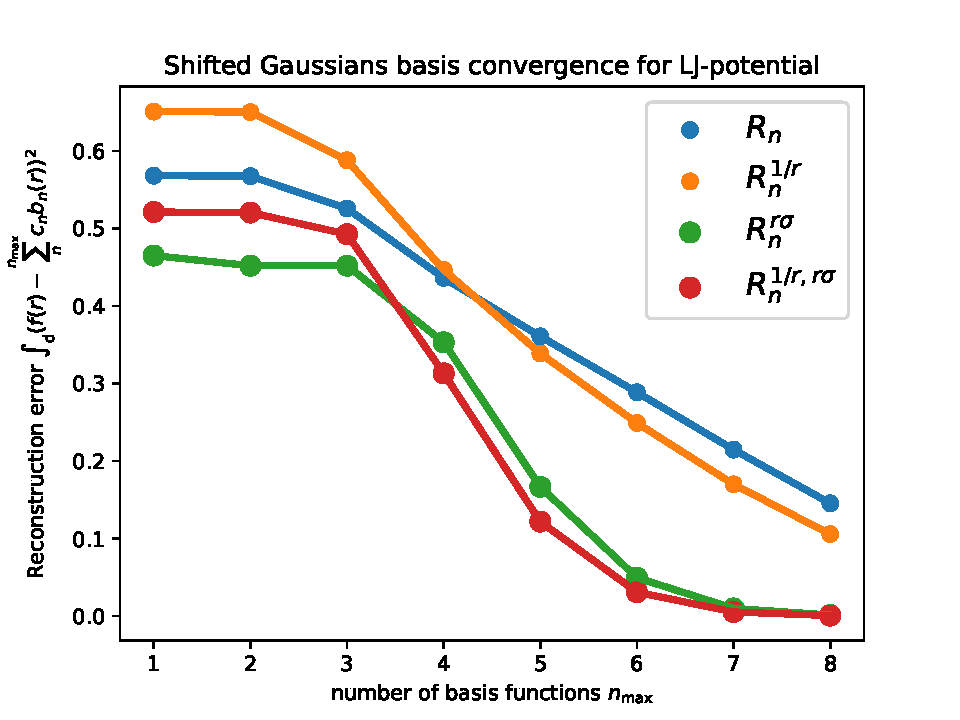
\includegraphics[width=\textwidth]{fig/convergence_results-grid500.pdf}
%    \caption{Comparison of the effect of radial scaling terms on the basis reconstruction for the LJ potential with the parameters $\epsilon_\textrm{LJ}=1.0$, $\sigma_\textrm{LJ}=1.1$ on the interval [1.05, 3.0]. A radial scaling in form of a global factor and in the smearing of the Gaussian $\sigma$ are compared.}
%    \label{fig:radial-scaling}
%    % TODO maybe plot basis and LJ potential
%\end{figure}
%Due to the duality expressed in Equation~\eqref{TODO} the reconstruction error is a reformulation of the mean-squared linear regression error of the energy determined by the defined LJ potential assuming uniform sampling.
%Numerous cases of interest however do not have a clear functional form as the LJ potential (e.g. neural network representations) such that this approach becomes unapplicable.
%%Furthermore Often the intervals of interest are not easy expressable.
%Furthermore, in the case of the LJ potential we purposefully did not include the range close to $0$ as the target function explodes and a reconstruction error would be dominated by that range providing not much insight.
%For higher-body orders the control of the intervals of interest becomes more complicated to embedd in the analysis.
%In the next section we show an approach to tackle these problems.
%
%%with the embedding of radial dependent on the $\sigma$ term for a LJ potential.
%%verify the effect of the redial scaling on LJ potential.
%%For th
%%\papercomment{We can also compare GTO and shifted Gaussian for LJ potential of dimers and should see that GTOs work better. Here we use numerical integration}
%%\papercomment{We can also compare GTO and and shifted Gaussian for LJ potential of dimers and should see that GTOs work better. Here we use numerical integration}
%
%\section{Formulation as optimization problem}
%%Furthermore, even if a functional form exists for high order functions (see Equation~\eqref{eq:integration_over_subgroup_higher_order}) such that a numerical integration becomes costly for higher-orders due to the polynomial cost of the integration wrt. the dimension of the integration space.
%%But even for order $2$ a numerical integration is costly when conducted over a large dataset.
%To address the problems discussed in the last section we reformulate the integration problem into an optimization problem that can be solved more efficiently.
%%with a scaling wrt. the number of basis functions
%%\begin{equation}
%%  \mathbf{c}\mathbf{B} = \mathbf{f},
%%  n, n x infty = infty (infty theoretical speaking)
%%  min_c \|\mathbf{f} - \mathbf{c}\mathbf{B}\| = loss
%%\end{equation}
%\begin{equation}
%  \label{eq:reconstruction_error_basis}
%  %\ell(\{c_nb_n\}^M_{n=1}, \{c^\prime_kb^\prime_k\}^M_{n=1}) = \| T(\{c_nb_n(r)\}_{n=1}^N) - c_kb_k^\prime(r)\|^2
%  \ell(\{c_nb_n\}^M_{n=1}, \{c^\prime_kb^\prime_k\}^M_{n=1}) = \int_D\mathrm{d}\mathbf{q}
%  \|\mathbf{T}(\mathbf{c}_\mathbf{q}\odot\mathbf{b}(\mathbf{q})) - \mathbf{c}^\prime_\mathbf{q}\odot\mathbf{b}^\prime(\mathbf{q})\|^2,\quad \mathbf{c},\mathbf{b}\in\mathbb{R}^{n_\textrm{max}}, \mathbf{T}\in\mathbb{R}^{n_\textrm{max}\times n^\prime_\textrm{max}}
%\end{equation}
%Assuming an orthonormal basis we obtain
%\begin{equation}
%  \label{eq:reconstruction_error_basis_coefficients}
%  %\ell(\{c_nb_n\}^M_{n=1}, \{c^\prime_kb^\prime_k\}^M_{n=1}) = \| T(\{c_nb_n(r)\}_{n=1}^N) - c_kb_k^\prime(r)\|^2
%  \ell(\{c_nb_n\}^M_{n=1}, \{c^\prime_kb^\prime_k\}^M_{n=1}) = \int_D\mathrm{d}\mathbf{q}
%  \|\mathbf{T}\mathbf{c}_\mathbf{q} - \mathbf{c}^\prime_\mathbf{q}\|^2
%\end{equation}
%Assuming orthogonormality can be a restrictive assumption.
%We can see the dependency on the orthonormalization matrix $\mathbf{S}^{-\frac12}$ on the target features
%\begin{subequations}
%\begin{align}
%  \min_\mathbf{T} \|\mathbf{T}\mathbf{c}_\mathbf{q} - \mathbf{S}^{-\frac12}\mathbf{c}^\prime_\mathbf{q}\|^2 
%  \leq \|\mathbf{S}^{-\frac12}\|^2 \min_\mathbf{T} \|\mathbf{T}\mathbf{c}_\mathbf{q} - \mathbf{c}^\prime_\mathbf{q}\|^2.
%  %  &= \min_\mathbf{T} \|\mathbf{S}^{\frac12}\mathbf{S}^{-\frac12}\mathbf{T}\mathbf{c}_\mathbf{q} - \mathbf{c}^\prime_\mathbf{q}\|^2 \\
%  %  &= \min_\mathbf{T} \|\mathbf{S}^{-\frac12}\mathbf{T}\mathbf{c}_\mathbf{q} - \mathbf{c}^\prime_\mathbf{q}\|^2 \\
%  %  &= \min_{\mathbf{T}} \|\mathbf{T}\mathbf{c}_\mathbf{q} - \mathbf{c}^\prime_\mathbf{q}\|^2 
%%   = \min_\mathbf{T} \|\mathbf{U}^T\mathbf{T}\mathbf{c}_\mathbf{q} - \mathbf{c}^\prime_\mathbf{q}\|^2 \\ %global unitary transformation is norm preserving
%%   = \min_\mathbf{T} \|\mathbf{T}\mathbf{c}_\mathbf{q} - \tilde{\mathbf{c}}^\prime_\mathbf{q}\|^2 \\
%%  %\ell(\{c_nb_n\}^M_{n=1}, \{c^\prime_kb^\prime_k\}^M_{n=1}) = \| T(\{c_nb_n(r)\}_{n=1}^N) - c_kb_k^\prime(r)\|^2
%%\|\mathbf{T}(\mathbf{c}_\mathbf{q}\odot\mathbf{b}(\mathbf{q})) - \mathbf{c}^\prime_\mathbf{q}\odot\mathbf{b}^\prime(\mathbf{q})\|^2
%%= \|\mathbf{T}(\mathbf{c}_\mathbf{q}\odot\mathbf{b}(\mathbf{q})) - \mathbf{U}\mathbf{c}^\prime_\mathbf{q}\odot\mathbf{b}^\prime(\mathbf{q})\|^2,
%%= \|\mathbf{U}^T\mathbf{T}(\mathbf{c}_\mathbf{q}\odot\mathbf{b}(\mathbf{q})) - \mathbf{c}^\prime_\mathbf{q}\odot\mathbf{b}^\prime(\mathbf{q})\|^2,
%%\tilde{c}_k\tilde{b}_k = (\sum_{i} U_{ki}c_{i})(\sum_{i} U_{ki}b_{i}(\mathbf{q})) = (\sum_{ij} U_{ki}U_{kj}c_{i}b_{j}(\mathbf{q}))
%\end{align}
%\end{subequations}
%This expresses just the general dependency of the error on linear transformations of the target function when no full reconstruction is possible.
%Assume a reconstruction of $\{(1, 0)_1, (0, 1)_2\}$ by coefficients $\{(1, 0)_1, (1, 0)_2\}$.
%By introducing a linear transformation to the targeted coefficients, the error can be made arbitrary large.
%This is crucial since it limits the insights we can get about the feature relationship, since a full rank linear transformation of the features does not reduce regression performance, but vice-versa the reconstruction error.
%For analysis that still can be related the meaning of Equation~\eqref{eq:reconstruction_error_basis} we therefore have to use an orthonormal basis for the target features.
%In this case a full rank orthonormality matrix can be absorbed by the linear transformation so we have equivalance to the orthonormal coefficients
%\begin{subequations}
%\begin{align}
%  \min_\mathbf{T} \|\mathbf{T}\mathbf{c}_\mathbf{q} - \mathbf{c}^\prime_\mathbf{q}\|^2.
%    = \min_\mathbf{T} \|\mathbf{T}\mathbf{S}^{-\frac12}\mathbf{c}_\mathbf{q} - \mathbf{c}^\prime_\mathbf{q}\|^2,
%  %  &= \min_\mathbf{T} \|\mathbf{S}^{\frac12}\mathbf{S}^{-\frac12}\mathbf{T}\mathbf{c}_\mathbf{q} - \mathbf{c}^\prime_\mathbf{q}\|^2 \\
%  %  &= \min_\mathbf{T} \|\mathbf{S}^{-\frac12}\mathbf{T}\mathbf{c}_\mathbf{q} - \mathbf{c}^\prime_\mathbf{q}\|^2 \\
%  %  &= \min_{\mathbf{T}} \|\mathbf{T}\mathbf{c}_\mathbf{q} - \mathbf{c}^\prime_\mathbf{q}\|^2 
%%   = \min_\mathbf{T} \|\mathbf{U}^T\mathbf{T}\mathbf{c}_\mathbf{q} - \mathbf{c}^\prime_\mathbf{q}\|^2 \\ %global unitary transformation is norm preserving
%%   = \min_\mathbf{T} \|\mathbf{T}\mathbf{c}_\mathbf{q} - \tilde{\mathbf{c}}^\prime_\mathbf{q}\|^2 \\
%%  %\ell(\{c_nb_n\}^M_{n=1}, \{c^\prime_kb^\prime_k\}^M_{n=1}) = \| T(\{c_nb_n(r)\}_{n=1}^N) - c_kb_k^\prime(r)\|^2
%%\|\mathbf{T}(\mathbf{c}_\mathbf{q}\odot\mathbf{b}(\mathbf{q})) - \mathbf{c}^\prime_\mathbf{q}\odot\mathbf{b}^\prime(\mathbf{q})\|^2
%%= \|\mathbf{T}(\mathbf{c}_\mathbf{q}\odot\mathbf{b}(\mathbf{q})) - \mathbf{U}\mathbf{c}^\prime_\mathbf{q}\odot\mathbf{b}^\prime(\mathbf{q})\|^2,
%%= \|\mathbf{U}^T\mathbf{T}(\mathbf{c}_\mathbf{q}\odot\mathbf{b}(\mathbf{q})) - \mathbf{c}^\prime_\mathbf{q}\odot\mathbf{b}^\prime(\mathbf{q})\|^2,
%%\tilde{c}_k\tilde{b}_k = (\sum_{i} U_{ki}c_{i})(\sum_{i} U_{ki}b_{i}(\mathbf{q})) = (\sum_{ij} U_{ki}U_{kj}c_{i}b_{j}(\mathbf{q}))
%\end{align}
%\end{subequations}
%so we only constrain the targeted feature space to be orthonormal if we want to retrieve Equation~\eqref{eq:reconstruction_error_basis}.
%On the other hand reconstruction of a nonorthonormal basis can still be justified by the fact that until the limit of convergence is not reached even a full rank linear transformations affects the regularization and thus also effects the regression performance.
%%Furthemore, even in the limit of convergence when comparing NN features, we can argue that the optimizers find similar local minimas with a similar $\|S\|$ factor %TODO for that argument I would need to dig into literature and change also the equation (find an equality relationship)
%
%%Instead of optimizing for the target function we optimize on a generic expansion. 
%%Similarly to the fact that we do not know in cases of interest the target function, we do not know if the basis expansion is orthonormal.
%%However, as orthonormalization is just a full rank linear transformation, we can assume it can be absorbed by $\mathbf{T}$.
%%\begin{subequations}
%%\begin{align}
%%  \min_\mathbf{T} \|\mathbf{T}\mathbf{c}_\mathbf{q} - \mathbf{S}^{-\frac12}\mathbf{c}^\prime_\mathbf{q}\|^2 
%%  \leq \|\mathbf{S}^{-\frac12}\|^2 \min_\mathbf{T} \|\mathbf{T}\mathbf{c}_\mathbf{q} - \mathbf{c}^\prime_\mathbf{q}\|^2 
%%  %  &= \min_\mathbf{T} \|\mathbf{S}^{\frac12}\mathbf{S}^{-\frac12}\mathbf{T}\mathbf{c}_\mathbf{q} - \mathbf{c}^\prime_\mathbf{q}\|^2 \\
%%  %  &= \min_\mathbf{T} \|\mathbf{S}^{-\frac12}\mathbf{T}\mathbf{c}_\mathbf{q} - \mathbf{c}^\prime_\mathbf{q}\|^2 \\
%%  %  &= \min_{\mathbf{T}} \|\mathbf{T}\mathbf{c}_\mathbf{q} - \mathbf{c}^\prime_\mathbf{q}\|^2 
%%%   = \min_\mathbf{T} \|\mathbf{U}^T\mathbf{T}\mathbf{c}_\mathbf{q} - \mathbf{c}^\prime_\mathbf{q}\|^2 \\ %global unitary transformation is norm preserving
%%%   = \min_\mathbf{T} \|\mathbf{T}\mathbf{c}_\mathbf{q} - \tilde{\mathbf{c}}^\prime_\mathbf{q}\|^2 \\
%%%  %\ell(\{c_nb_n\}^M_{n=1}, \{c^\prime_kb^\prime_k\}^M_{n=1}) = \| T(\{c_nb_n(r)\}_{n=1}^N) - c_kb_k^\prime(r)\|^2
%%%\|\mathbf{T}(\mathbf{c}_\mathbf{q}\odot\mathbf{b}(\mathbf{q})) - \mathbf{c}^\prime_\mathbf{q}\odot\mathbf{b}^\prime(\mathbf{q})\|^2
%%%= \|\mathbf{T}(\mathbf{c}_\mathbf{q}\odot\mathbf{b}(\mathbf{q})) - \mathbf{U}\mathbf{c}^\prime_\mathbf{q}\odot\mathbf{b}^\prime(\mathbf{q})\|^2,
%%%= \|\mathbf{U}^T\mathbf{T}(\mathbf{c}_\mathbf{q}\odot\mathbf{b}(\mathbf{q})) - \mathbf{c}^\prime_\mathbf{q}\odot\mathbf{b}^\prime(\mathbf{q})\|^2,
%%%\tilde{c}_k\tilde{b}_k = (\sum_{i} U_{ki}c_{i})(\sum_{i} U_{ki}b_{i}(\mathbf{q})) = (\sum_{ij} U_{ki}U_{kj}c_{i}b_{j}(\mathbf{q}))
%%\end{align}
%%\end{subequations}
%% loss is the same for orthogonormal coefficients 
%%\mathbf{c}_\mathbf{q}
%%TODO problem if \mathbf{b}^\prime(\mathbf{q}) not orthogonal
%
%%For a normalized basis functions such a transformation implies an upper bound on the dataset for any linear relationship that can be build with the targeted feature space
%%\begin{equation}
%%  \label{eq:transformation}
%%  \sum_{n=1}^M \|\sum_k T(c_kb_k) - y \|^2 \leq ...
%%\end{equation}
%%We therefore can make a more general statement about any target functions wrt. to a transformation relating the targeted feature space to $y$ for a dataset. 
%%therefore focus on the development of error measurements as in Equation~\eqref{eq:information_capacity} that provide quantative results for the information capacity of feature spaces and that are efficient to compute.
%%a numerical integration in the high-order space is also not feasible
%%the density for Section~\ref{eq:radial_angular_density} 
%%\begin{equation}
%%  \ell(\{c_kb_k\}^M_{k=1}, f) = \int_V\mathrm{d}\mathbf{q}\, \|\sum_{k=1}^M c_kb_k(\mathbf{q}) - f(\mathbf{q})\|.
%%\end{equation}
%%We can now evaluate the expression for existing datasets, but we can also assume a distribution of $r_{ji}$ 
%
%%Another approach that can also provide more insights into the interdependency between represenations is to express the convergence rate
%% orthonormalized basis we can compare the function approximation error of the
%%original basis by
%%for the presented basis.
%%We can see the results in Figure \papercomment{TODO} that the quality of the GTO
%%\papercomment{
%%Compare here DVR, GTO, Bartok on some example function
%%}
%%surpasses all the mentioned basis functions. 
%%That is unsurprising since the GTO is modeled towards the central atomic density
%%approach.
%%The function approximation error however does not implicate that a similar trend
%%will be observed for property prediction error. \\
%%\papercomment{Use this to build up motivation for unusupervised metrics as GFRE, since
%%we need to run this on a grid and this does not work in high dimensional space.}
%%
%%% ---
%%
%%More formally speaking, a set of basis functions with the best convergence behavior
%%wrt. to some error measure.
%%\begin{equation}
%%\ell(\{c_n\}_n, \{b_n\}_n, f)
%%\end{equation}
%%In the QSAR case we would target the L2-norm prediction error of the property.
%%\begin{equation}
%%\ell(\{c_n\}_n, \{b_n\}_n, f) = \int\mathrm{d}\mathbf{r}\, \|\tilde{g}(\sum_n c_nb_n(\mathbf{r})) - g(f(\mathbf{r}))\|
%%\end{equation}
%%\papercomment{a bit to abstract at the moment}
%%
%%\papercomment{
%%\begin{itemize}
%%  \item quality of basis function depends on function to represent
%%\end{itemize}
%%}
%
%%In order to compare two separate sets of features, one can employ regression errors to quantify the mutual relationships of different forms of featurizations. %, as demonstrated in \cite{Goscinski2021}.
%%We determine this error, or the feature reconstruction measure (FRM), by reconstructing one set of features from the other with a constrained transformation, where different constraints express different types of relationships between the two sets of features.
%%
%%Say we have a dataset that is represented in full detail by a representation \Ftrue, and we want to assess the amount of information lost by using an alternate representation \Fone. We can check the detail contained in \Fone~by computing FRM(\Fone, \Ftrue), where $\text{FRM} = 0$ corresponds to a perfect reconstruction with no loss, and $\text{FRM} \approx 1$ denotes a complete information loss wrt. \Ftrue. 
%%However, there rarely exists a ground-truth representation \Ftrue\, and we are more commonly comparing two likely-imperfect representations \Fone\ and \Ftwo. In this case, we compute FRM(\Fone, \Ftwo) and FRM(\Ftwo, \Fone). The feature set that results in the higher reconstructive measure is considered higher in information capacity (e.g.~if FRM(\Fone, \Ftwo) $>$ FRM(\Ftwo, \Fone), then \Fone\ is the more information-rich feature set). The advantage of the FRM is that it can give quantitative results about the shared information content between two sets of features, even without the existence of a ground truth.
%%
%%In Figure \ref{fig:frm} we show a schematic of the different FRMs. 
%%The simplest FRM is the global feature reconstruction error (GFRE), expressed as the linearly decodable information, as given by performing ridge regression between the two sets of features.
%%We note that in the case of choosing the property as ground truth, the GFRE is equivalent to a regression task on the standardized property.
%%The global feature reconstruction distortion (GFRD) constrains the transformation to be orthogonal to demonstrate the deformation incurred by transforming between the two feature spaces.
%%
%%Extending the analysis to non-linear dependencies, the local feature reconstruction error (LFRE) applies ridge regression for each point locally on the $k$-nearest neighbors.
%%These methods are of particular use in assessing the hyperparameters of ML descriptors\cite{goscinski2021role} and have been employed to compare the efficiency of different basis sets in encoding geometrical information\cite{musil2021physics, goscinski2021optimal}.
%
%In the following sections we show error measures based on the loss in Equation~\eqref{eq:reconstruction_error_basis_coefficients} that constraint the transformation $\mathbf{T}$ to provide different insights to the feature-relationship.
%In Figure~\ref{fig:frm} a schematic of the different types of transformations $T$ that are covered in the upcoming sections.
%These methods are of particular use in assessing the hyperparameters of ML descriptors\cite{goscinski2021role} and have been employed to compare the efficiency of different basis sets in encoding geometrical information\cite{musil2021physics, goscinski2021optimal}.
%
%\begin{figure*}
%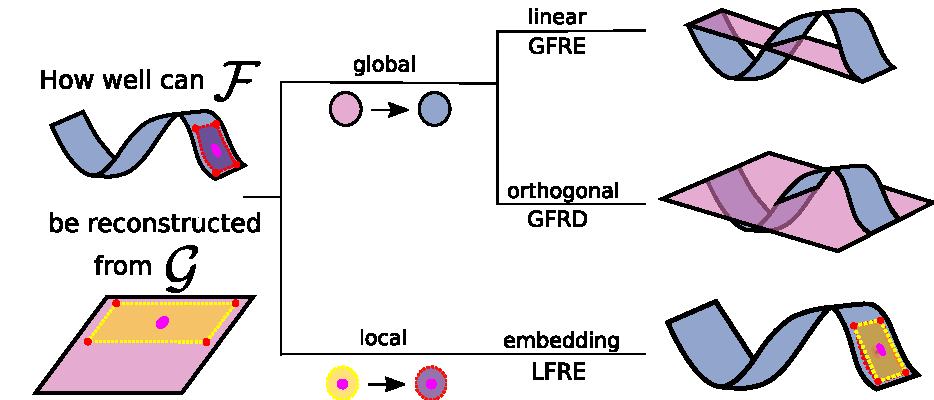
\includegraphics[width=\linewidth]{fig/frm.pdf}
%% Titles and legends: Each figure or table should have a concise title of no more than 15 words. A legend for each figure and table should also be provided that briefly describes the key points and explains any symbols and abbreviations used. The legend should be sufficiently detailed so that the figure or table can stand alone from the main text.
%\caption{\textbf{The different forms of feature reconstructions}
%to assess two feature spaces (blue and pink) describing the same dataset. Here, we are reconstructing the curved manifold (blue) using the planar manifold (pink), as it is often the case to approximate a complex manifold with a simpler alternative. The area framed by the dotted line is an example of a local neighborhood of one sample (the pink dot) that enables the reconstruction of nonlinearities. (Top) The linear transformation is used in the global feature reconstruction error (GFRE). (Middle) The orthogonal transformation is used in the global feature reconstruction distortion (GFRD). (Bottom) A local linear transformation of a neighborhood is used in local feature reconstruction error (LFRE). On the right, the reconstructions of the manifold are drawn in pink together with the curved manifold in blue. The measures correspond to the root-mean-square difference between the reconstructed and curved manifold.
%}\label{fig:frm}
%\end{figure*}
%
%
%\section{Linear decodable information}
%The FRMs differ in two aspects: the locality of the reconstruction (global or local) and the constraints of the regression. In each FRM, the two feature sets are partitioned into training and testing sets. We standardise the features of \Fone~and \Ftwo~ individually, then we regress the features of \Fone~onto \Ftwo~ to compute the errors. In the global measures, we use the entire dataset for the reconstruction, whereas in the local measure, we perform a regression for each sample on the set of the $k$-nearest points within \Fone. The number $k$ is given by the user with the parameter \texttt{n\_local\_points}. The \emph{reconstruction error} is by default computed using a 2-fold cross-validation (CV) and ridge regression as estimator. 
%
%As most interesting applications use large feature vectors, we implemented a custom 2-fold ridge to improve computational efficiency.
%In \texttt{slearn}, an implementation of the leave-one-out CV with a similar purpose of speeding up the CV exists.
%\papercomment{Put here some results on the comparison contained in the examples of skmatter}
%%For the reconstruction \emph{distortion} we use orthogonal regression as implemented in \texttt{OrthogonalRegression} in the \texttt{\skmatshort.linear\_model} module.
%
%As a simple, easily-interpretable measure of the relative expressive power of $\CF$ and $\CF^\prime$, we introduce the global feature space reconstruction error $\GFRE^\CD(\CF,\CF^\prime)$, defined as the mean-square error that one incurs when using the feature matrix $\bX_\CF$ to linearly regress $\bX_{\CF^\prime}$. 
%In this work we compute the $\GFRE$ by a 2-fold split of the dataset, i.e. compute the regression weights $\bP{\CF}{\CF^\prime}$ over a train set $\CDtr$ composed of half the entries in $\CD$,
%\begin{equation}
%\begin{split}
%\bP{\CF}{\CF^\prime}= &
%\operatorname{argmin} \bP{}{}\in\BR^{\nf_{\CF}\times\nf_{\CF^\prime}}
%\norm{\bX^{\CDtr}_{\CF^\prime} - \bX^{\CDtr}_{\CF} \bP{}{}  }\\
%=&\left({\bX_{\CF}^{\CDtr}}^T \bX_{\CF}^{\CDtr}\right)^{-1}
%(\bX_{\CF}^{\CDtr})^T\bX_{\CF^\prime}^{\CDtr}
%\end{split}\label{eq:proj-ff1}
%\end{equation}
%and then compute the error over the remaining test set $\CDte$
%\begin{equation}
%\GFRE^\CD(\CF,\CF^\prime) = \sqrt{{\norm{\bX^{\CDte}_{\CF^\prime} - \bX^{\CDte}_{\CF} \bP{\CF}{\CF^\prime}  }^2}/\ns_\test},
%\label{eq:GFRE}
%\end{equation}
%averaging, if needed, over multiple random splits.  The $\GFRE$ is a positive quantity, which is equal to zero when there is no error in the reconstruction, and that is usually bound by one\footnote{This is due to the fact that feature matrices are standardized, and so $\norm{\bX^{\CDte}_{\CF^\prime}}/\ns_\test $ is of the order of one}.
%
%Notice that by expressing the basis and target functions on a radial grid basis we retrieve the numerical integration loss in Equation~\eqref{TODO}.
%The minimization problem is moved from an optimization of $\mathbf{c}$ to an optimization of $\mathbf{W}$.
%%to solving for $M\times n_\textrm{grid}$.% matrix retrieving the expansion coefficients.
%While the former requires to solve the loss for each datapoint the later only needs one the whole dataset.
%As solving the minimization problem has worst scaling behavior in the computation of the loss, the later approach is typically more efficient to compute.
%%an$c_k$ changes for datapoint and $M\times n_\textrm{grid}$ is constant over samples.
%%In the limit of number basis function for $f$, thus we obtain a similar loss as the numerical integration in Equation~\eqref{TODO} where target function is evaluated on some grid to compute the integral.
%
%For numbers of features larger than $\ns_\train$, the covariance matrix is not full rank, and one needs to compute a pseudoinverse. Without loss of generality, one can regularize the regression to stabilize the calculation. In this paper, we computed the pseudoinverse by means of a singular value decomposition, and we determined the optimal regularization in terms of the truncation of the singular value spectrum, using 2-fold cross-validation over the training set to determine the optimal truncation threshold. Often, it is also useful to observe the behavior of the $\GFRE$ in the absence of any regularization: overfitting is in itself a signal of the instability of the mapping between feature spaces.
%In general, $\GFRE^\CD(\CF,\CF^\prime)$ is not symmetric. If $\GFRE^\CD(\CF,\CF^\prime)\approx\GFRE^\CD(\CF^\prime,\CF)\approx 0$, $\CF$ and $\CF^\prime$ contain similar types of information; if $\GFRE^\CD(\CF,\CF^\prime)\approx 0$, while $\GFRE^\CD(\CF^\prime,\CF)>0$, one can say that $\CF$ is more descriptive than $\CF^\prime$: this is the case, for instance, one would observe if $\CF^\prime$ consists of a sparse version of $\CF$, with some important and linearly-independent features removed; finally, if  $\GFRE^\CD(\CF,\CF^\prime)\approx\GFRE^\CD(\CF^\prime,\CF)>0$, the two feature spaces contain different, and complementary, kinds of information and it may be beneficial to combine them to achieve a more thorough description of the problem.
%
%\subsection{Effficient cross-validation ridge for high-dimensional feature space}
%
%In linear regression, the complexity of computing the weight matrix is
%theoretically bounded by the inversion of the covariance matrix.  This is
%more costly when conducting regularized regression, wherein we need to
%optimise the regularization parameter in a cross-validation (CV) scheme,
%thereby recomputing the inverse for each parameter.  scikit-learn offers an
%efficient leave-one-out CV (LOO CV) for its ridge regression which avoids
%these repeated computations \cite{loocv}. Because we needed an efficient ridge that works
%in predicting  for the reconstruction measures in  metric
%we implemented in \texttt{skmatter} an efficient 2-fold CV ridge regression that uses a singular value decomposition
%(SVD) to reuse it for all regularization parameters $\lambda$. Assuming
%we have the standard regression problem optimizing the weight matrix in
% 
%\begin{align}
%  \|\mathbf{X}\mathbf{W} - \mathbf{Y}\|
%\end{align}
% 
%Here $\mathbf{Y}$ can be seen also a matrix as it is in the case of
%multi target learning. Then in 2-fold cross validation we would predict first
%the targets of fold 2 using fold 1 to estimate the weight matrix and vice
%versa. Using SVD the scheme estimation on fold 1 looks like this.
%                                                                                      
%\begin{align}
%    &\mathbf{X}_1 = \mathbf{U}_1\mathbf{S}_1\mathbf{V}_1^T,
%          \qquad\qquad\qquad\quad
%          \textrm{feature matrix }\mathbf{X}\textrm{ for fold 1} \\
%    &\mathbf{W}_1(\lambda) = \mathbf{V}_1
%           \tilde{\mathbf{S}}_1(\lambda)^{-1} \mathbf{U}_1^T \mathbf{Y}_1,
%           \qquad
%           \textrm{weight matrix fitted on fold 1}\\
%    &\tilde{\mathbf{Y}}_2 = \mathbf{X}_2 \mathbf{W}_1,
%           \qquad\qquad\qquad\qquad
%           \textrm{ prediction of }\mathbf{Y}\textrm{ for fold 2}
%\end{align}
%
%The efficient 2-fold scheme in `Ridge2FoldCV` reuses the matrices
%                                                                                      
%\begin{align}
%    &\mathbf{A}_1 = \mathbf{X}_2 \mathbf{V}_1, \quad
%     \mathbf{B}_1 = \mathbf{U}_1^T \mathbf{Y}_1.
%\end{align}
%                                                                                      
%for each fold to not recompute the SVD. The computational complexity
%after the initial SVD is thereby reduced to that of matrix multiplications.
%
%We can see that Leave-one-out CV is estimating the error wrong for low
%alpha values. That seems to be a numerical instability of the method. If we
%would have limit our alphas to 1E-5, then LOO CV would have reach similar
%accuracies as the 2-fold method.
%
%We note that this is not an fully encompasing comparison
%covering sufficient enough the parameter space. We just want to note that in
%cases with high feature size and low effective rank the ridge solvers in
%skmatter can be numerical more stable and act on a comparable speed.
%                                                                              
%
%\subsubsection{Cutoff and Tikhonov regularization}
%When using a hard threshold as regularization (using parameter ``cutoff``),
%the singular values below $\lambda$ are cut off, the size of the
%matrices $\mathbf{A}_1$ and $\mathbf{B}_1$ can then be reduced,
%resulting in further computation time savings.  This performance advantage of
%\emph{cutoff} over the \emph{Tikhonov} is visible if we to predict multiple targets
%and use a regularization range that cuts off a lot of singular values. For
%that we increase the feature size and use as regression task the prediction
%of a shuffled version of $\mathbf{X}$.
%
%
%We can see that a regularization value of 1e-8 cuts off a lot of singular
%values. This is crucial for the computational speed up of the
%\emph{cutoff regularization method}
%
%\subsection{Example: Wasserstein distance}
%As an example of the transformation induced by a non-Euclidean metric we consider the effect of using a Wasserstein distance to compare $\nu=1$ density correlation features. 
%The Wasserstein distance (also known as the Earth Mover Distance, EMD) is defined as the minimum  ``work^{\prime}^{\prime} that is needed to transform one probability distribution into another -- with the work defined as the amount of probability density multiplied by the extent of the displacement~\cite{vall74siam,cohe-guib97report,cutu07proc}.
%The EMD has been used to define a ``regularized entropy match^{\prime}^{\prime} kernel to combine local features into a comparison between structures~\cite{de+16pccp}, to obtain permutation-invariant kernels based on Coulomb matrices\cite{ccaylak2020wasserstein}, and  has been shown to be equivalent to the Euclidean distance between vectors of sorted distances~\cite{will+19jcp}.
%Here we use the Wasserstein distance to compare two-body ($\nu=1$) features, that can be expressed on a real-space basis and take the form of one-dimensional probability distributions. 
%% MC  this looks like an entirely general definition >> More formally, for an atomic environment with cutoff $r_c$, we can define the $\nu$-body 
%
%The formal definition of the Wasserstein distance of order 2 between two probability distributions $p(r)$ and $p^{\prime}(r)$ defined on a domain $M$ reads
%\begin{equation}
%W(p,p^{\prime})^2 = \hspace{-1em}\inf_{\gamma\in\Gamma (p,p^{\prime})} \int_{M\times M}\hspace{-0.5em}d(r,r^{\prime})^2\,\mathrm{d}\gamma(r,r^{\prime}),
%%W_2(p_{\mathcal{X}_i},p_{\mathcal{X}_j})^2 = \hspace{-1em}\inf_{\gamma\in\Gamma (p_{\mathcal{X}_i},p_{\mathcal{X}_j})} \int_{M\times M}\hspace{-0.5em}d(r,r^{\prime})^2\,\mathrm{d}\gamma(r,r^{\prime}),
%%
%%W_2(p_{\mathcal{X}^{(\nu)}_i},p_{\mathcal{X}^{(\nu)}_j})^2 = \hspace{-1em}\inf_{\gamma\in\Gamma (p_{\mathcal{X}_i^{(\nu)}},p_{\mathcal{X}_j^{(\nu)}})} \int_{M^{\nu}\times M^{\nu}}\hspace{-2.5em}d(r,r^{\prime})^2\,\mathrm{d}\gamma(r,r^{\prime}), Adding many body order makes it too cluttered
%%\mathcal{X}_i = \int_{M^{\nu}} \gamma(x,x^{\prime})\,\mathrm{d}x I would not write this out because \mathcal{X} is not a probability distribution without any transformation, this way we keep the definition of \Gamma open
%\end{equation}
%where $\Gamma(p,p^{\prime})$ is the set of all joint distributions with marginals $p$ and $p^{\prime}$.
%For 1-dimensional distributions, $W(p,p^{\prime})$ can be expressed as the 2-norm of the difference between the associated inverse cumulative distribution function (ICDF) $P^{-1}$ of two environments,
%$W(p,p^{\prime})^2=\int_0^1  \left|P^{-1}(s) -{P^{\prime}}^{-1}(s)\right|^2\D{s}$, with $P(r)=\int_0^r p(r)\D{r}$ 
%
%In order to express the symmetrized 2-body correlation function as a probability density, we first write it on a real-space basis $\rep<r|$, and evaluate it on 200 Gaussian quadrature points, that we also use to evaluate the CDF and its inverse. 
%We then proceed to normalize it, so that it can be interpreted as a probability density.
%We estimate the integral of the distribution (that effectively counts the number of atoms within the cutoff distance) 
%\begin{equation}
%Z_i = \int_0^{r_c}\rep< r||A;\frho_i^1>\,\mathrm{d}r,
%\end{equation}
%and the maximum value of the integral over the entire dataset $Z_\CD$.
%A simple scaling of the correlation function 
%\begin{equation}
%p_i^{\text{s}}(r) = \frac1{Z_i} \rep< r||A;\frho_i^1>\label{eq:wass-pis}
%\end{equation}
%distorts the comparison between environments with different numbers of atoms.
%To see how, we use the \emph{displaced methane} dataset, in which three atoms in a $\textrm{CH4}$ molecule are held fixed in the ideal tetrahedral geometry, at a distance of 1\AA{} from the carbon centre. The fourth atom, aligned along the $z$ axis, is displaced along it, so that each configuration is parameterised by a single coordinate $\zh$.
%Figure~\ref{fig:wasserstein-distances}(a) shows the distance computed between pairs of configurations with different $\zh$,  demonstrating the problem with the renormalized probability~\eqref{eq:wass-pis}: $p^{\text{s}}$ loses information on the total number of atoms within the cutoff, and so once the tagged atom moves beyond $r_\text{c}$ the remaining \ce{CH3} environment becomes indistinguishable from an ideal \ce{CH4} geometry. 
%
%One can obtain a more physical behavior when atoms enter and leave the cutoff by introducing a $\delta$-like ``sink^{\prime}^{\prime} at the cutoff distance, defining
%\begin{equation}
%p^{\delta}_i(r) = \frac{1}{Z_\CD}\left[\rep< r||\mathcal{A};\frho_i^1> + (Z_\CD-Z_i)\delta(r-r_c)\right].
%\end{equation}
%Figure~\ref{fig:wasserstein-distances}b shows that with this choice the Wasserstein metric between $p_i^\delta(r)$ reflects the distance between the moving atoms. With this normalization, in fact, the Wasserstein metric corresponds to a smooth version of the Euclidean metric computed between vectors of sorted interatomic distances~\cite{will+19jcp}, shown in Figure~\ref{fig:wasserstein-distances}c. 
%The distortions that can be seen in the comparison between Figure~\ref{fig:wasserstein-distances}b,c are a consequence of the Gaussian smearing, the smooth cutoff function, and the $\SOthree$ integration that modulates the contribution to $\rep< r||\mathcal{A};\frho_i^1>$ coming from atoms at different distances.
%
%Having defined a meaningful normalization and a probabilistic interpretation of the radial density correlation features, we can investigate how the feature space induced by a Wasserstein metric relates to that induced by an Euclidean distance. 
%Figure~\ref{fig:wasserstein-grid} shows the error in the reconstruction of $\zh$ for the \emph{displaced methane} dataset when restricting the training set to 0.05\AA{} and 1.0\AA{} spaced grids.
%Using a Euclidean distance with a sharp $\sigmag$ leads to a highly non-linear mapping between the displacement coordinate and feature space, and a linear model cannot interpolate accurately between the points of a sparse grid. 
%A Wasserstein metric, on the other hand, measures the minimal distortion needed to transform one structure into another, and so provides a much more natural interpolation along $\zh$, which is robust even with a sharp density and large spacing between training samples. 
%It is worth stressing that the sorted distance metric -- which effectively corresponds to the $\delta$ density limit of the Wasserstein metric -- performs rather poorly, and cannot even reproduce the training points.
%This is because the mapping between feature space and $\zh$ is not exactly linear, changing slope when $\zh$ crosses 1\AA{} (because the sorting of the vector changes)  and 4\AA{} (because one atom exits the cutoff). The sorted-distances feature space does not have sufficient flexibility to regress this piecewise linear map, as opposed to its smooth Wasserstein counterpart.
%
%\begin{figure}
%\includegraphics[width=1\linewidth]{fig/distance_comparison-delta_wasserstein-carbon-inkscaped.pdf}
%\caption{Comparison of GFRE and GFRD for the \emph{carbon} dataset, using sharp ($\sigmag=0.1$\AA{}) and smooth ($\sigmag=0.5$\AA{}) radial SOAP features, as well as Euclidean (E) and Wasserstein (W) metrics.}
%\label{fig:wasserstein-carbon}
%\end{figure}
%
%Having rationalized the behavior of the Wasserstein metric for a toy model, we can test how it compares to the conventional Euclidean metric on a more realistic data set. We consider in particular the AIRSS \emph{carbon} data set, and compare different levels of density smearing as well as Euclidean and Wasserstein metrics. 
%Figure~\ref{fig:wasserstein-carbon} paints a rather nuanced picture of the relationship between the linear and the Wasserstein-induced feature spaces. 
%The GFRE is non-zero in both directions, meaning that (in a linear sense) Wassertein and Euclidean features provide complementary types of information. 
%Smearing of the density has a small effect on the Wasserstein metric, so that both $\GFRE(W(\sigmag=0.1\text{\AA}),W(\sigmag=0.5\text{\AA}))$ and $\GFRD(W(\sigmag=0.1\text{\AA}),W(\sigmag=0.5\text{\AA}))$ are small, whereas for Euclidean features -- as observed in Section~\ref{sub:hypers} -- changing $\sigmag$ induces small information loss, but a large distortion of feature space. 
%Overall, there is no sign of the pathological behavior seen in Figure~\ref{fig:wasserstein-grid}, which is an indication that (at least for 2-body features) the \emph{carbon} dataset is sufficiently dense, and that the better interpolative behavior of the EMD does not lead to a more informative feature space. 
%
%\subsection{Example: Comparison of bispectrum and message-passing}
%\papercomment{Put in Jigyasa^{\prime}s work where the GFRE was used to compare MP with 3-body.}
%
%\section{Distortion in linear transformations}
%The feature space reconstruction error gives insights into whether a feature space can be inferred by knowledge of a second one. However, having both a small $\GFRE^\CD(\CF,\CF^\prime)$ and $\GFRE^\CD(\CF^\prime,\CF)$ does not imply two feature spaces are identical. Even though they contain similar amounts of information, one feature space could give more emphasis to some features compared to the other, which can eventually result in different performance when building a model.
%To assess the amount of distortion of $\CF^\prime$ relative to $\CF$, we introduce the global feature space reconstruction distortion $\GFRD^\CD(\CF,\CF^\prime)$.
%To evaluate it, we first compute the singular value decomposition of the projector Equation~\eqref{eq:proj-ff1}, $\bP{\CF}{\CF^\prime}\approx\bU \bSIG \bV^T$, and then use it to reduce the two feature spaces to a common basis, in which the reconstruction error is zero, because the residual has been discarded
%\begin{equation}
%\bXt_{\CF} = \bX_{\CF}\bU \quad  \bXt_{\CF^\prime} = \bXt_{\CF} \bSIG.
%\end{equation}
%When the second feature space $\CF^\prime$ has a lower dimensionality than $\CF$, some combinations of the starting features are not used to compute $\tilde{\CF}^\prime$. 
%In this case, we pad $\bSIG$ with zeros, so that $\tilde{\CF}^\prime$ has the same dimensionality $\nf_{\CF}$ as the starting space. This choice ensures that the GFRD takes the same value it would have in the case $\CF^\prime$ had the same dimensionality as $\CF$, but lower rank. 
%In the opposite case, with $\nf_{\CF}<\nf_{\CF}^\prime$, padding $\bSIG$ and $\bU$ with zeros, or truncating $\bV$, yields the same $\GFRD$.
%
%We can then address the question of whether $\bXt_{\CF}$ and $\bXt_{\CF^\prime}$ are linked by a unitary transformation (in which case the $\GFRD$ should be zero), or there is a distortion involved.
%A possible answer involves solving the orthogonal Procrustes problem~\cite{scho66pm} -- i.e. finding the orthogonal transformation that ``aligns^{\prime}^{\prime} as well as possible $\bXt_{\CF}$ to $\bXt_{\CF^\prime}$:
%\begin{equation}
%\begin{split}
%\bQ{\CF}{\CF^\prime} =& \operatorname{argmin}\bQ{}{} \in \mathbb{U}^{\nf\times\nf}
%\norm{\bXt^{\CDtr}_{\CF^\prime} - \bXt^{\CDtr}_{\CF} \bQ{}{}  }\\
%=&\tilde{\bU}\tilde{\bV}^T,
%\end{split}\label{eq:proc-ff1}
%\end{equation}
%where $\tilde{\bU}\tilde{\bSIG}\tilde{\bV}^T = (\bXt_{\CF}^{\CDtr})^T \bXt^{\CDtr}_{\CF^\prime}$ .
%The amount of distortion can then be computed by assessing the residual on the test set,
%\begin{equation}
%\GFRD^\CD(\CF,\CF^\prime) = \sqrt{{\norm{{\bXt}^{\CDte}_{\CF^\prime} - {\bXt}^{\CDte}_{\CF} \bQ{\CF}{\CF^\prime}  }^2}/\ns_\test}. \label{eq:GFRD}
%\end{equation}
%If desired, the error can be averaged over multiple random splits of the reference data set $\CD$.
%
%%\subsection{Effect of zero dimensions} TODO
%%\papercomment{Here I can embed the example from skmatter}
%
%\subsection{Example: Radial scaling}
%
%One of the most important hyperparameters when defining an atom-centred representation is the cutoff distance, which restricts the contributions to the density to the atoms with $r_{ji}<r_{\text{c}}$.
%Figure~\ref{fig:soap-sigma-radial-body}(c,d) shows that the GFRE captures the loss of information associated with an aggressive truncation of the environment, with very similar behavior between GTO and DVR bases. 
%The figure also reflects specific features of the different data sets: for instance, $\GFRE(r_\text{c}=4\,\text{\AA},r_\text{c}=6\,\text{\AA})$ is close to zero for the random methane data set, because there are no structures where atoms are farther than $4\,$\AA{} from the centre of the environment. $\GFRE>0$ also when mapping long-cutoff features to short-range features, although the reconstruction error is much smaller than in the opposite direction. 
%This indicates the need for an increase in $\nmax$ to fully describe the structure of an environment when using a large value of $r_\text{c}$, which is consistent with the greater amount of information encoded within a larger environment.
%The GFRD plot also underscores the strong impact of the choice of $r_\text{c}$ on the emphasis that is given to different parts of the atom-density correlations. 
%This effect explains the strong dependency of regression performance on $r_\text{c}$, and the success of multi-scale models that combine features built on different lengthscales~\cite{bart+17sa}. 
%A similar modulation of the contributions from different radial distances can be achieved by scaling the neighbor contribution to the atom-centred density by a decaying function, e.g. $1/(1+(r_{ji}/r_0)^s)$. This approach has proven to be very effective in fine-tuning the performance of regression models using density-based features~\cite{fabe+17jctc,will+18pccp,paru+18ncomm}.
%As shown in Figure~\ref{fig:soap-sigma-radial-body}(e,f), this is an example of a transformation of the feature space that entails essentially no information loss -- resulting in a very small GFRE between different values of the scaling exponent $s$. However, it does result in substantial $\GFRD$, providing additional evidence of how the emphasis given by a set of features to different inter-atomic correlations can affect regression performance even if it does not remove altogether pieces of structural information.
%
%%The effect of the radial scaling on the features is compared by multiplying the density~\eqref{eq:density} with $r^q$ where $q$ is the radial scaling exponent.
%%With higher distance between the radial scaling exponents the distortion between features is more significant, while the information is mostly preserves as seen in Figure~\ref{fig:soap-sigma-radial-body}c),d).
%
%\begin{figure*}
%    \includegraphics[width=0.9\linewidth]{fig/sigma_radial_scaling_cutoff_comparison-gfrd-gto_dvr-methane_carbon-inkscaped-v2.pdf}
%    \caption{Comparison of the GFRE (top) and GFRD (bottom) a),b) for different smearing  $\sigma_G$ ($r_\text{c}=4\,$\AA{}) c),d) for different cutoff values ($\sigmag=0.5\,$\AA), and e),f) for different radial scaling exponents ($r_\text{c}=4\,$\AA{}, $\sigmag=0.5\,$\AA). For all comparisons $(\nmax,\lmax) = (10,6)$ were used. The feature specified by the row is used to reconstruct the feature specified by the column.}
%    \label{fig:soap-sigma-radial-body}
%\end{figure*}
%
%\section{Nonlinearity as local linearity}
%The limitation to linear transformations allows us to efficiently compute the loss over a dataset, but also restricts us from describing nonlinear relationships.
%A branch of models are based on NNs and apply nonlinearities to an initial representation to obain their final one.
%As these models are also often opaque in their learned representation, it is essential to develop a measure that can also work for nonlinearities.
%%Even higher-body orders are type of nonlinear nonlinearities is interesting to analyze
%
%In principle for the transformation $T$ in Equation~\eqref{eq:fre_transformationTODO} a neural network could be used that model nonlinearities.
%Neural networks are however usually only efficient in the prediction of a few target properties and not large number of features where convergence might be unfeasible.
%In addition NNs have a lot model parameters that need to be chosen (e.g. activation function, number of layers) making the loss highly dependent on the exact architecture which makes it hard to make general statements.
%
%In this Section we discuss ways to model nonlinearities the linearities and its limitations.
%We propose for future directions to restrict the type of nonlinearities carefully which still allows to answer certain research questions.
%%and are therefore unsuitable for such an application,
%%result would change 
%%give interpretable quantative measure. Incorperating
%
%\subsection{Local linear embedding}
%%A downside of the global feature comparison schemes introduced above is that the linear nature of the regression means that they cannot detect if $\CF$ and $\CF^\prime$ contain analogous information, but differ by a non-linear transformation.
%%In the next Section we discuss how one can generalize the schemes to use kernel features, that can also be used to detect non-linear relationships between the original feature spaces.
%%\newcommand{\CDki}{\CD_{k-\text{neigh}}^{(i)}}
%An alternative approach is to compute a local version of the feature space reconstruction error, $\LFRE^\CD(\CF,\CF^\prime)$, loosely inspired by locally-linear embedding~\cite{rowe-saul00science}. 
%To compute the LFRE, a local regression is set up, computed in the $k$-neighborhood $\CDki$ around sample $i$  -- the set of $k$ nearest neighbors of sample $i$, based on the Euclidean distance between the samples in $\CF$ -- to reproduce the $\CF^\prime$ features using $\CF$ as input features, centred around their mean values $\bar{\bx}_{\CF^\prime}$ and $\bar{\bx}_{\CF}$.
%
%
%A local embedding of $\bx_i$ is determined as
%\begin{equation}
%\tilde{\bx}^\prime_i = \bar{\bx}_{\CF^\prime} + (\bx_i - \bar{\bx}_{\CF})\bP{\CF}{\CF^\prime}^{(i)},\label{eq:xtilde_lle}
%\end{equation}
%where $\bP{\CF}{\CF^{\prime}}^{(i)}$ contains the regression weights computed from $\CDki$.
%The local feature space reconstruction error is given by the residual discrepancy between the $\CF^\prime$ counterpart of the $i$-th point and its local embedding~\eqref{eq:xtilde_lle}:
%\begin{equation}
%\LFRE^\CD(\CF,\CF^\prime) = \sqrt{\sum_i \norm{\bx^\prime_i - \tilde{\bx}^\prime_i}^2/{\ns_\test}}.
%\label{eq:LFRE}
%\end{equation}
%Inspecting the error associated with the reconstruction of individual points can reveal regions of feature space for which the mapping between $\CF$  and $\CF^\prime$ is particularly problematic. 
%Similarly, one can compute a local version of $\GFRD$, that could be useful to detect strong local distortions that might indicate the presence of a singularity in the mapping between two feature spaces.
%
%\subsubsection{Example - Degeneracies in 3-body features}
%The LFRE also makes it possible to identify regions of phase space for which the construction of a mapping between feature spaces is difficult or impossible. 
%Consider the case of the degenerate manifold discussed in Ref.~\citenum{pozd+20prl}. The dataset includes two sets of \ce{CH4} environments, and those parameterised by $v=0$ cannot be distinguished from each other using 3-body ($\nu=2$) features.
%Figure~\ref{fig:soap_degenerated_manifold_lfre} shows the LFRE for each point along the two manifolds. When trying to reconstruct 3-body features using as inputs 4-body features (that take different values for the two manifolds) the LFRE is essentially zero. When using the 3-body features as inputs, instead, one observes a very large error for points along the degenerate line, while points that are farther along the manifold can be reconstructed well. This example demonstrates the use of the LFRE to identify regions of feature space for which a simple, low-body-order representation is insufficient to fully characterize the structure of an environment, and can be used as a more stringent, explicit test of the presence of degeneracies than the comparison of pointwise distances discussed in Ref.~\citenum{pozd+20prl}. 
%
%\begin{figure}
%    \centering
%    \includegraphics[scale=0.42]{fig/lfre-body_order_comparison-nb_local_neighbors=15-degenerated_manifold.png}
%\caption{Pointwise LFRE for the structures from the degenerate methane dataset as a function of the structural coordinates $(u,v)$ for $(\nmax,\lmax) = (6,4)$ and $k=15$ neighbors.}
%    \label{fig:soap_degenerated_manifold_lfre}
%\end{figure}
%
%\subsection{Jacobian}
%For an atomic environment the rows of a Jacobian matrix correspond to the spatial directions of the atoms in the environment.
%A row describes the change of the features with respect to a change in the corresponding spatial direction of the atom.
%\begin{figure}
%    \centering
%    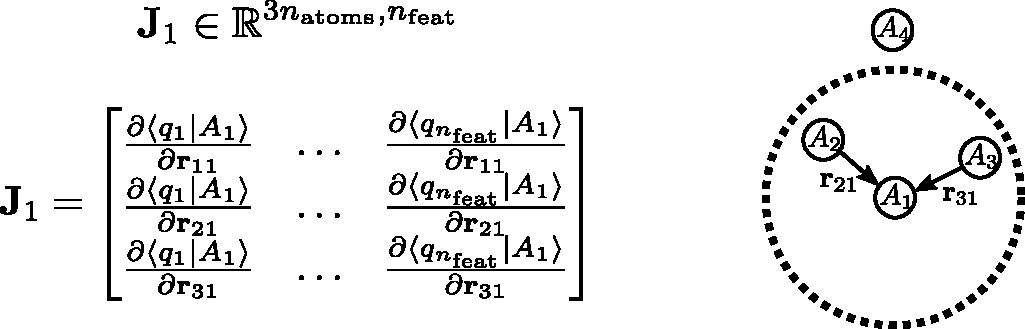
\includegraphics[width=\textwidth]{fig/jacobian.pdf}
%    \caption{Sketch of the Jacobian matrix of ACDC features for atomic environment $A_1$. The dashed circle represents the cutoff of the environment.}
%    \label{fig:jacobian}
%\end{figure}
%If we treat the Jacobian reconstruction as a classical linear learning problem, then these rows represent the sample dimension.
%The number of atoms within an environment is in reasonable settings very small.
%Due to this very small number of samples, the generalization error cannot be well approximated using cross-validation.
%%Adding atoms into an environment changes features intrinsically.
%%In the latter case we can deduct the regularization parameter by cross-validation.
%%In the local case, however, due to the low number of samples this procedure becomes statistically unreliable.
%%In principle with enough numerical precision the Jacobian reconstruction errors is always zero as long as the precision of the reconstruction is below the numerical noise of the calculation of the features.
%%In this cas
%%Nevertheless, we can still extract certain information from the reconstruction error of the Jacobian about the information capacity of the features.
%%The matrix captures the change of the represention under inifinitesmall changes of neighboring atoms in one of the spatial direction.
%We therefore need a different method to determine a regularization term that can be seen as an estimation of the noise in the features.
%Rank deficiencies in the Jacobian matrix correspond to linearly dependent directions with the same change in features.
%Each symmetry embedded in the features results in a deficiency in the Jacobian matrix.
%In our setting there are three deficiencies due to translational symmetries and three due to rotational.
%Additional deficiencies exist due to structure-specific symmetries (see Figure~\ref{fig:jacobian-symmetry}), or due to directions that the features cannot represent.
%\begin{figure}
%    \centering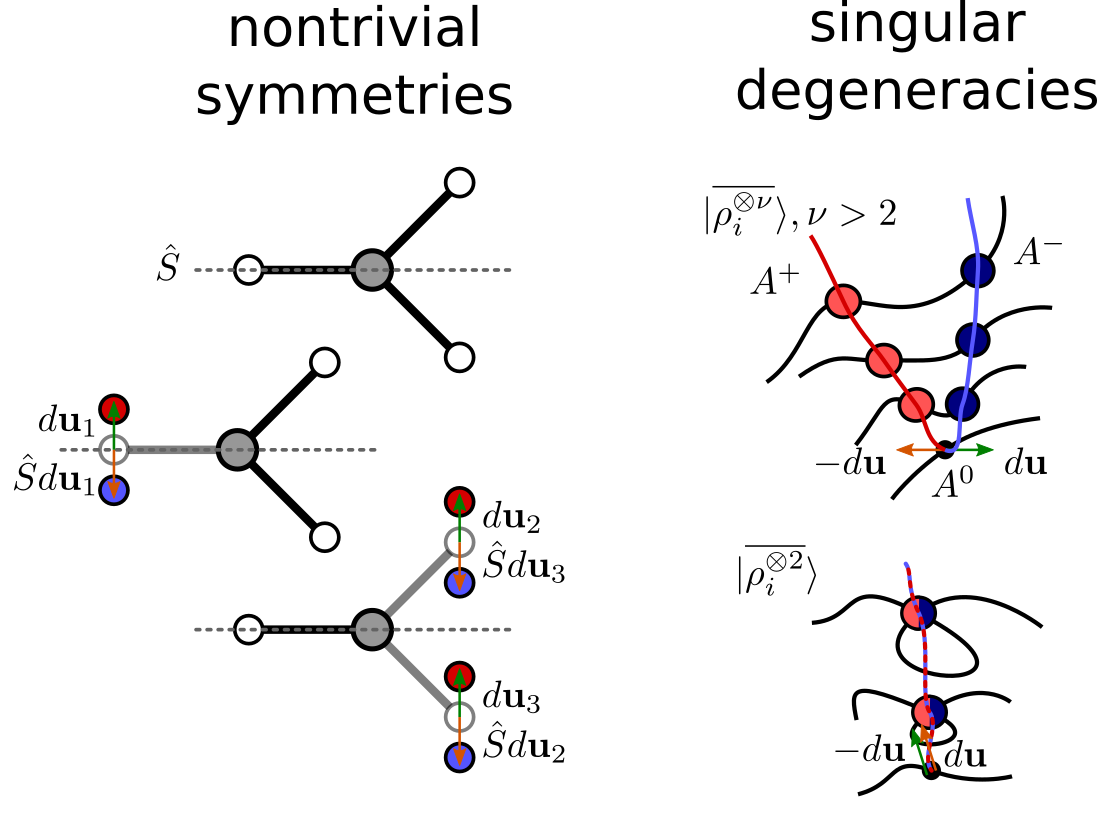
\includegraphics[width=0.8\textwidth]{fig/jacobian_rank_deficiencies}
%    \caption{Sketch of nontrivial rank deficiencies in the Jacobian matrix in case of nontrivial symmetries or singular degeneracies. Adapted from Ref.~\cite{localinvertibility2021pozdnyakov}.}
%    \label{fig:jacobian-symmetry}
%\end{figure}
%In the latter case it is the intersection of degenerate manifolds, manifolds of pointwise different environments but with the same features, that create these singular points with deficiencies\cite{localinvertibility2021pozdnyakov}.
%%What distinguishes the information capacity of features are the deficiencies because of the latter case\cite{sergey}.
%To express a Jacobian reconstruction error, we worked on a method for finding a reasonable threshold cutting off singular values corresponding to such deficient directions.
%%For a directly-interpretable experimental results it is important to determine the rank accurately which has been one challene of the current work.
%
%\subsubsection{Machine precision for rank estimation}
%%Numerically the rank of a matrix is determined by counting the singular values above a certain threshold relative to the largest singular value of the matrix.
%Since we are in control of the whole computation of the features up to the singular values, errors are introduced even due to the machine precision of the number format or to mathematical numerical approximations in the features computation.
%%To estimate the final error due to machine precision of the number format in the computation of the singular values.
%One approach for the estimation of the error due to machine precision would require an error estimation of the computation starting from the featurization of the atom^{\prime}s positions up to the singular value decomposition of the Jacobian matrix.
%%While in principle this approach is possible to implement, 
%The error estimations of each mathematical operation have to be chained together to one final estimation.
%Analytical bounds are however too loose and require probabilistic considerations to be reasonable tight for our application\cite{huynh2011error}.
%%Furthermore the error analyivsis needs a propagation through the whole computation of the Jacobian which is not a feasible approach considering the amount of work to rewrite the software.
%Least-square solvers in SciPy and NumPy use a heuristic for the threshold dependent on the machine precision of number format (for float $\approx1.19\mathrm{e}{-7}$, for double $\approx2.22\textrm{e}{-16}$) and the maximal dimension of the matrix $\mathbf{J}\in\mathbb{R}^{m,n}$
%\begin{multline}
%  \tau_\textrm{numpy} = \eta\cdot\max(n,m),\textrm{ where }\eta\textrm{ is number format dependent unit roundoff.}
%\end{multline}
%For most cases of interest, the heuristic gives reasonable thresholds, see Figure~\ref{fig:svals-unsupervised-separation}a).
%But in cases it produces disputable thresholds, where the singular values are close to the threshold, it is hard to justify that the term $\max(n,m)$ is the correct prefactor for features with arbitrary hyperparameters, as for example in the case of low number of basis functions in Figure~\ref{fig:svals-unsupervised-separation}b).
%
%\subsubsection{Signal-noise separation for rank estimation}
%Another approach assumes that the singular values corresponding to signal and to noise are well-separable.
%This characteristic of well-separability can be expressed into different conditions depending on the context.
%In the case of independent component analysis (ICA) it is that the noise is statistically independent from the signal. 
%For rank estimation the approach of Ref.~\cite{JMLR:v9:braun08a} assumes that the singular values have different orders of magnitude.
%The rank $\hat{d}$ maximizes the likelihood of two Gaussians $\mathcal{N}(0, \sigma_\textrm{signal})$ and $\mathcal{N}(0, \sigma_\textrm{noise})$ describing the singular value probability density function.
%By optimizing their standard deviation $\sigma_\textrm{signal}$ and $\sigma_\textrm{noise}$ the estimated rank is
%\begin{equation}
%    \hat{d} = \textrm{argmin}_{1\leq d\leq n} (\frac{d}{n}\log(\sigma_\textrm{signal}^2) + \frac{n-d}{n} \log\sigma_\textrm{noise}^2 ).
%\end{equation}
%In cases of sufficient number of basis function, no radial scaling and reasonable smearing sigma as in Figure~\ref{fig:svals-unsupervised-separation}a) a clear separation of the singular values can be achieved.
%%\ref{subfig:svals-unsupervised-separation-large}.
%Such constraints are not for all cases of interest fulfilled and subsequently this method starts to fail in such cases Figure~\ref{fig:svals-unsupervised-separation}b) producing arbitrary rank estimations.
%\begin{figure}
%    \centering
%    \begin{subfigure}[b]{0.49\textwidth}
%        \centering
%        \includegraphics[width=0.8\textwidth]{fig/symmetry_sval_line-ps-nmax8-lmax6.png}
%        \label{subfig:svals-unsupervised-separation-large}
%        \caption{}
%    \end{subfigure}
%    \begin{subfigure}[b]{0.49\textwidth}
%        \centering
%        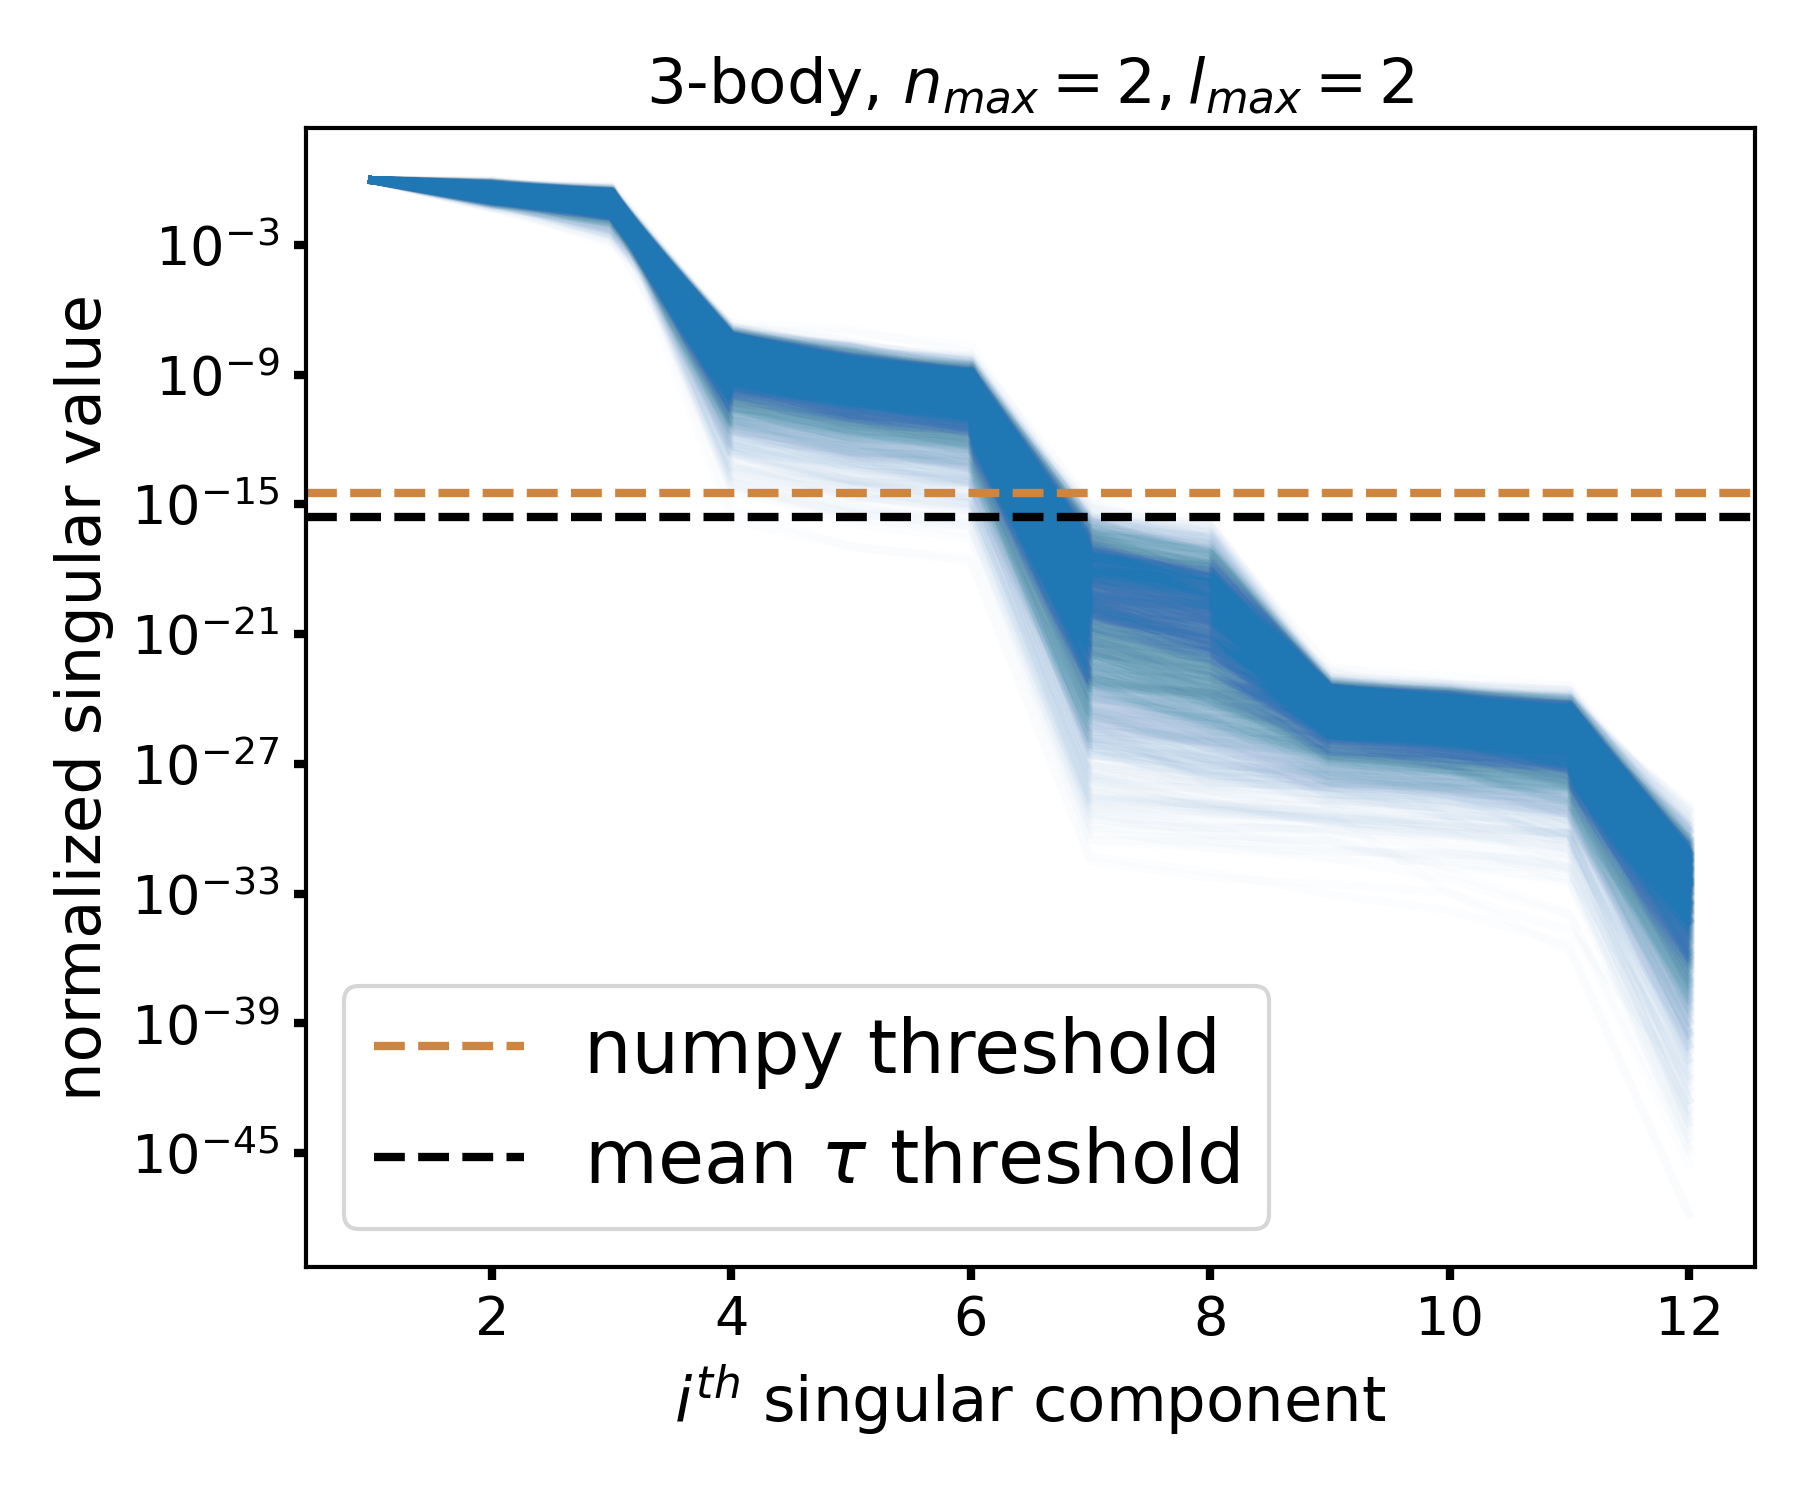
\includegraphics[width=0.8\textwidth]{fig/symmetry_sval_line-ps-nmax2-lmax2.png}
%        \label{subfig:svals-unsupervised-separation-small}
%        \caption{}
%    \end{subfigure}
%    \caption{
%        Singular value spectrum of the Jacobian of the carbon environments for several methane molecules. Different number of basis functions have been used to demonstrate the separability of the singular value spectrum for rank estimation.
%        The singular spectra are plotted with a high transparent value so that opaque regions correspond to numerous spectra going through.
%        We can see a) for a reasonably number of basis functions that the signal and the noise are well-separable while b) for a too small number this is note the case. 
%    }
%    \label{fig:svals-unsupervised-separation}
%\end{figure}
%
%\subsubsection{Exploiting symmetries for rank estimation}
%\begin{figure}
%    \centering
%    \includegraphics[width=\textwidth]{fig/random_global_translation.pdf}
%    %\begin{subfigure}[b]{0.3\textwidth}
%    %    \includegraphics[width=0.8\textwidth]{fig/rof/random_global_translation.png}
%    %    \label{fig:random-global-translation}
%    %\end{subfigure}
%    %\begin{subfigure}[b]{0.3\textwidth}
%    %    \includegraphics[width=0.8\textwidth]{fig/rof/symmetry_sval_hist-ps-nmax8-lmax6.png}
%    %    \label{fig:sval-hist-ps-nmax8-lmax6}
%    %\end{subfigure}
%    %\begin{subfigure}[b]{0.3\textwidth}
%    %    \includegraphics[width=0.8\textwidth]{fig/rof/symmetry_sval_line-ps-nmax8-lmax6.png}
%    %    \label{fig:sval-line-ps-nmax8-lmax6}
%    %\end{subfigure}
%    \caption{
%      The procedure for estimating the threshold for a Jacobian matrix $\mathbf{J}$. a) We sample directions corresponding to global translations which are invariant to features. b) By mapping these directions on the Jacobian matrix corresponding, we sample from a distribution of the numerical error over the features. c) Then we use the maximal numerical error over the features to estimate the threshold using Equation~\eqref{eq:threshold-random-matrix-theory}.}
%    \label{fig:threshold-estimation}
%\end{figure}
%
%From the last approach we can identify the core problem that the rank estimation becomes arbitrary in cases where no single clear gap exists.
%The question becomes how to deal with a certain amount of arbitrariness for these cases in a reasonable way while being mostly precise in cases where a single clear gap exist.
%To this end we exploit the null space spanned by the symmetries embedded in the features to retrieve the numerical error.
%Assuming that the numerical noise is isotropical in all directions $\sigma$ we can split our Jacobian matrix in information $\mathbf{X}$ and noise $\sigma \mathbf{Z}$, where $\mathbf{Z}$ are random entries from Gaussian distribution $[\mathbf{Z}]_{ij}\sim\mathcal{N}(0, 1)$
%\begin{equation}
%    \mathbf{J} = \mathbf{X} + \mathbf{Z}\sigma.
%\end{equation}
%By projecting with directions corresponding to symmetries $\hat{\mathbf{u}}$ with unit length onto $\mathbf{J}$ we obtain
%\begin{equation}
%    \hat{\mathbf{u}}\mathbf{J} = \hat{\mathbf{u}}\mathbf{X} + \hat{\mathbf{u}}\mathbf{Z}\sigma = \hat{\mathbf{u}}\mathbf{Z}\sigma,
%    \label{eq:sampling-numerical-noise}
%\end{equation}
%where the entries $[\hat{\mathbf{u}}\mathbf{Z}]_{ij}\sim\mathcal{N}(0,1)$ due to the unit length of $\hat{\mathbf{u}}$.
%By sampling from different directions $\hat{\mathbf{u}}$ we can sample from the entries in $\sigma\mathbf{Z}$, and thereby retrieve $\sigma$.
%Given the noise estimation we can use results from random matrix theory\cite{gavish2014optimal} to determine the optimal threshold value% in terms of the asymptotic mean squared error of the matrix reconstruction.
%\begin{multline}
%    \tau = \lambda(\beta)\sqrt{n}\sigma,\qquad \mathbf{J}\in\mathbb{R}^{m,n}, m\leq n, \beta = m/n,\\
%    \textrm{where }\lambda(\beta) = \sqrt{2(\beta+1)+\frac{8\beta}{(\beta+1)+\sqrt{\beta^2+14\beta+1}}},
%    \label{eq:threshold-random-matrix-theory}
%\end{multline}
%with respect to the asymptotic mean squared error between the truncated Jacobian matrix $\mathbf{J}_{\tau}$ and the actual information matrix $\mathbf{X}$.
%In this asymptotic setting the matrix dimension of $\mathbf{J}$ goes to infinity while the rank and ratio $\beta$ stays constant\cite{shabalin2013reconstruction}.
%%The threshold is optimal in terms of asymptotic mean squared error, increasing the size of the matrices by more.
%While the asymptotic threshold is not necessary optimal for the finite setting, it nevertheless gives decent results as discussed in Ref.~\cite{gavish2014optimal}.
%When we applied this threshold method on 3-body features we could see that the quality of the rank predictions depends highly on our noise estimation.
%We observed that the rank of the Jacobian matrix for 3-body features was overestimated for almost $\approx10\%$ of the carbon environments in the random methane dataset.
%The reason for this rank overestimation is that the noise is not isotropical distributed over the different features seen in Figure~\ref{fig:threshold-estimation}b).
%% and secondly that the numerical noise estimation does follow a larger tail than $\mathcal{N}(0, \sigma^2)$.
%To prevent these underestimations, we use the maximal noise over all features for the threshold computation as described in Figure~\ref{fig:threshold-estimation}.
%
%\subsection{Example: Message-passing and connectivity}
%A lot of development in the community has been targeted on message-passing models due to highly accurate predictions in the low data regime\cite{schutt2021equivariant,batzner20223}.
%Recent results have established that message-passing is essentially an efficient way of decomposing the space for higher resolution\cite{nigam2022unified}.
%It is however not clear what the effect of higher number of interactions in message-passing has on the capacity of environment features.
%Nonlinear effects due to the activation functions as well as due to the message-passing are usually entangled with each other in NN architectures and have not been fully understood yet.
%Considering domain decomposition parallelization as it is typically used in molecular dynamics software packages\cite{LAMMPS} message-passing prohibits an embarrassingly parallel problem over domains and even enforces a nontrivial communication between the CPUs/GPUs corresponding to the domains or an increase in the cutoff of the potential resulting in less room for parallelization.
%Especially, regarding recent results that achieve similar accurate predictions without message-passing\cite{musaelian2022learning} or with a minimal amount of message interactions\cite{batatia2022mace}, it is a valid question how much the more efficient decomposition of the geometric space due to message-passing contributes to the learning performance for learned short-range force fields.
%We have run preliminary experiments on a dataset with randomly displaced methane structures\cite{pozdnyakov2020dataset} using 2-body message-passing features\cite{schutt2018schnet} analysing the rank of the Jacobian matrix with respect to the number of interactions $m-1$
%\begin{equation}
%  \langle n00| \rho_i^{\otimes([1\leftarrow1])^{m}} \rangle\textrm{, 2-body message-passing features as in Ref.~\cite{nigam2022unified}}.
%    \label{eq:schnet-message-passing}
%\end{equation}
%We analyzed the ranks of the Jacobians corresponding to carbon environments with the method presented in Section~\ref{sec:threshold-estimaton}.
%We consider environments with a cutoff of $6$\AA where all atoms are connected with each other, and $3$\AA where all hydrogen atoms are connected with the carbon atom, but not necessary with all other hydrogen atoms.
%\begin{figure}
%    \centering
%    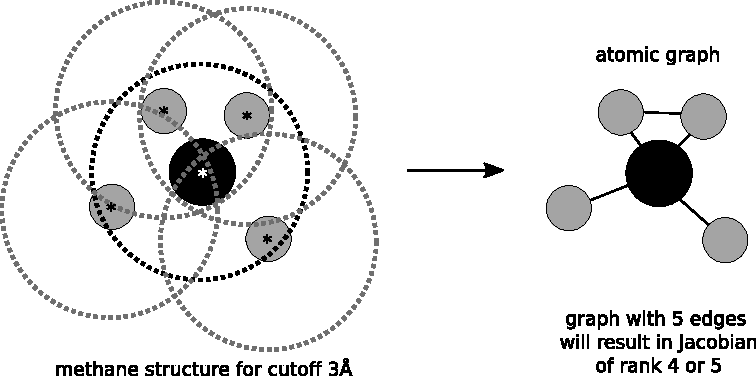
\includegraphics[width=\textwidth]{fig/atomic_graph.pdf}
%    \caption{Illustration of the atomic graph for one methane structure with a cutoff of $3$\AA.}
%    \label{fig:atomic-graph}
%\end{figure}
%It can observed in Figure~\ref{fig:threshold-estimation} that the rank does not increase after one interaction for any significant amount of the carbon environments.
%The maximum rank correlates well with the total number of edges in the graph with respect to the cutoff seen in Figure~\ref{fig:threshold-estimation}.
%%This preliminary results suggests that message-passing has only negligible effect on the information capacity of the features after one interaction.
%A simple explanation for this observation is that each edge can by reached two moves from the carbon environment.
%The correlation of the number of edges with the rank can be explained by the fact that we only deal with a finite system of 5 atoms in total.
%The number of edges grows as $n$ over $2$ while the largest possible rank grows as $3n-6$ due to symmetries.
%Thus for the methane dataset with a maximal number of edges $10$ and a maximal rank of $9$ there exist always one edge that adds linearly dependent information.
%Therefore the Jacobian rank must be within $[n_\textrm{edges}-1, n_\textrm{edges}]$ for all points in this dataset.
%We expect that for larger or periodic structures the rank will increase also after one interaction, as in this case every passed message can reach the the carbon atom within two steps
%%atom is connected with each other over carbon environment, resulting in a maximum node distance of 2.
%%So any additional inofrmaiton
%%due to missing connections to pass higher-body order information through the messages, which cannot be retrieved by algebraic operations of existing ones.
%%In Figure~\ref{} one can see a simple reason that
%\begin{figure}[h]
%    \centering
%    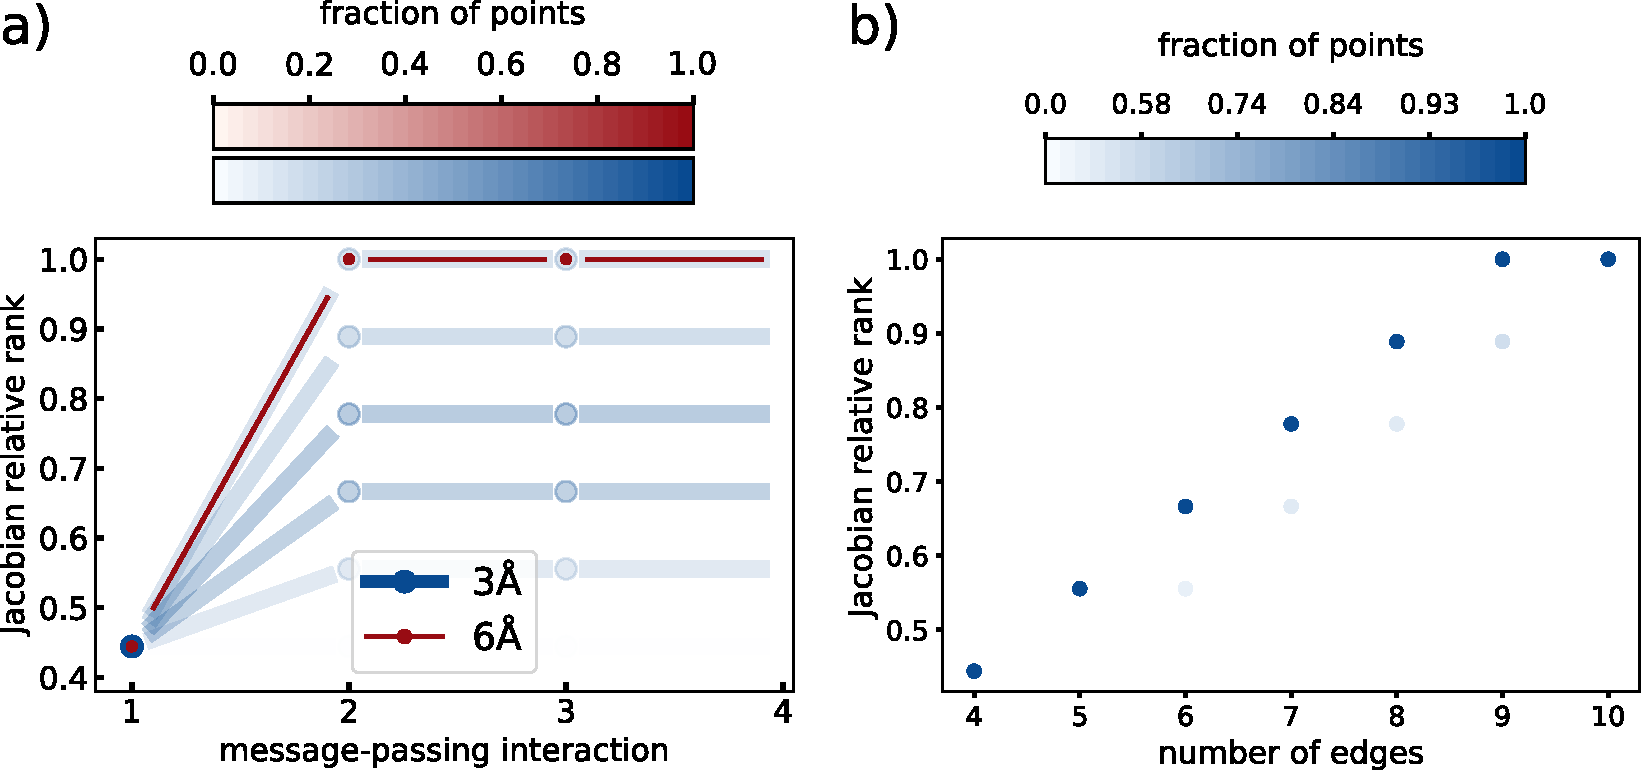
\includegraphics[width=\textwidth]{fig/ranks_CH-train-max_est-checkpoint0.pdf}
%    \caption{Rank estimations for the Jacobians of 2-body message-passing features for the carbon environments: a) the ranks with respect to increasing number of interactions, b) the ranks with respect to the number edges in the atomic graph for a cutoff of $3$\AA. The ranks are scaled such that the maximum possible rank $5\cdot3-6=9$ is normalized to $1.0$.}
%    \label{fig:message-passing-results}
%\end{figure}
%
%
%\subsection{Local stiffness [optional]}
%Even in the case of no degeneracies we want to express how stable a mapping from one feature space to another is in general.
%We want to differ the error between a mapping which changes in each point dramatically and a mapping which is nearly constant over the whole dataset.
%One way to approach this problem is to use higher-order derivatives extending the range with each order.
%However, already computing second-order derivatives is a computationally demanding task, higher-orders are not even feasible.
%We therefore developed a similar approach as the Tikhonov regularization.
%%Due to this we therefore decided to consider the error propagation over the whole relevant spectrum of regularizers.
%%One problem when considering the whole spectrum of regularizers is that we break the identity relationship.
%%Jacobian matrices with a more uniform eigenspectrum can even result in smaller errors than the identity relationship.
%Instead of penalizing the norm of the weight matrix, we penalize the change of the weight matrix between two points.
%\begin{align}
%\ell(X_1, \ldots, X_n, Y_1, \ldots, Y_n) =& \sum_i
%\|X_iW_i-Y_i\|^2 \nonumber \\
%&+ \beta\sum_{i\neq j}\frac{1}{d(\mathbf{x}_i,\mathbf{x}_j)+1}\|W_i-W_j\|^2\label{eq:nonlinearm}
%%&\ell = \sum_i\big(\|X_iW_i-Y_i\|^2 + \beta\sum_{i\neqj}\frac{c_i}{d(\mathbf{x}_i,\mathbf{x}_j)+1}\|W_i-W_j\|^2\big)
%%&c_i\textrm{ is solved by }\sum_{j\neq i} \frac{c_i}{d(\mathbf{x}_i-\mathbf{x}_j)+1} = 1 \\
%\end{align}
%An unstable map with significant changes in the weight matrices between points will be penalized and thus be pushed to more stable mapping with a larger error in the optimization.
%%if environments in the vicinity exist.
%In contrast, an identity map can be kept constant over the whole dataset and is thereby not affected by the penalization term.
%This term is closely related to a stretching energy term in the optimization of elastic maps\cite{kass1988snakes}.
%One can see for the toy example in Figure~\ref{fig:nonlinearm}c) mapping $x$ to $1$ that by increasing $\beta$ the mapping starts to break at the degenerate point at $x=0$.
%In Figure~\ref{fig:nonlinearm}b) the $1$-features and $0.5\sin(x)$ are compared, both reconstructing the $x$-features by optimizing the loss function described in Equation~\eqref{eq:nonlinearm}.
%We can see that initially $1$ to $x$ produces a smaller errors, since its eigenvalue spectrum is more uniform than $0.5\sin(x)$, while the mapping $0.5\sin(x)$ to $x$ gives smaller error for large $\beta$ values, because the feature mapping $0.5\sin(x)$ to $x$ requires fewer changes of the weights over the dataset than $1$ to $x$ and is thus more stable.
%Increasing $\beta$ even more results in the mapping constant over the whole dataset which recovers the global mapping.
%\begin{figure}
%    \centering
%    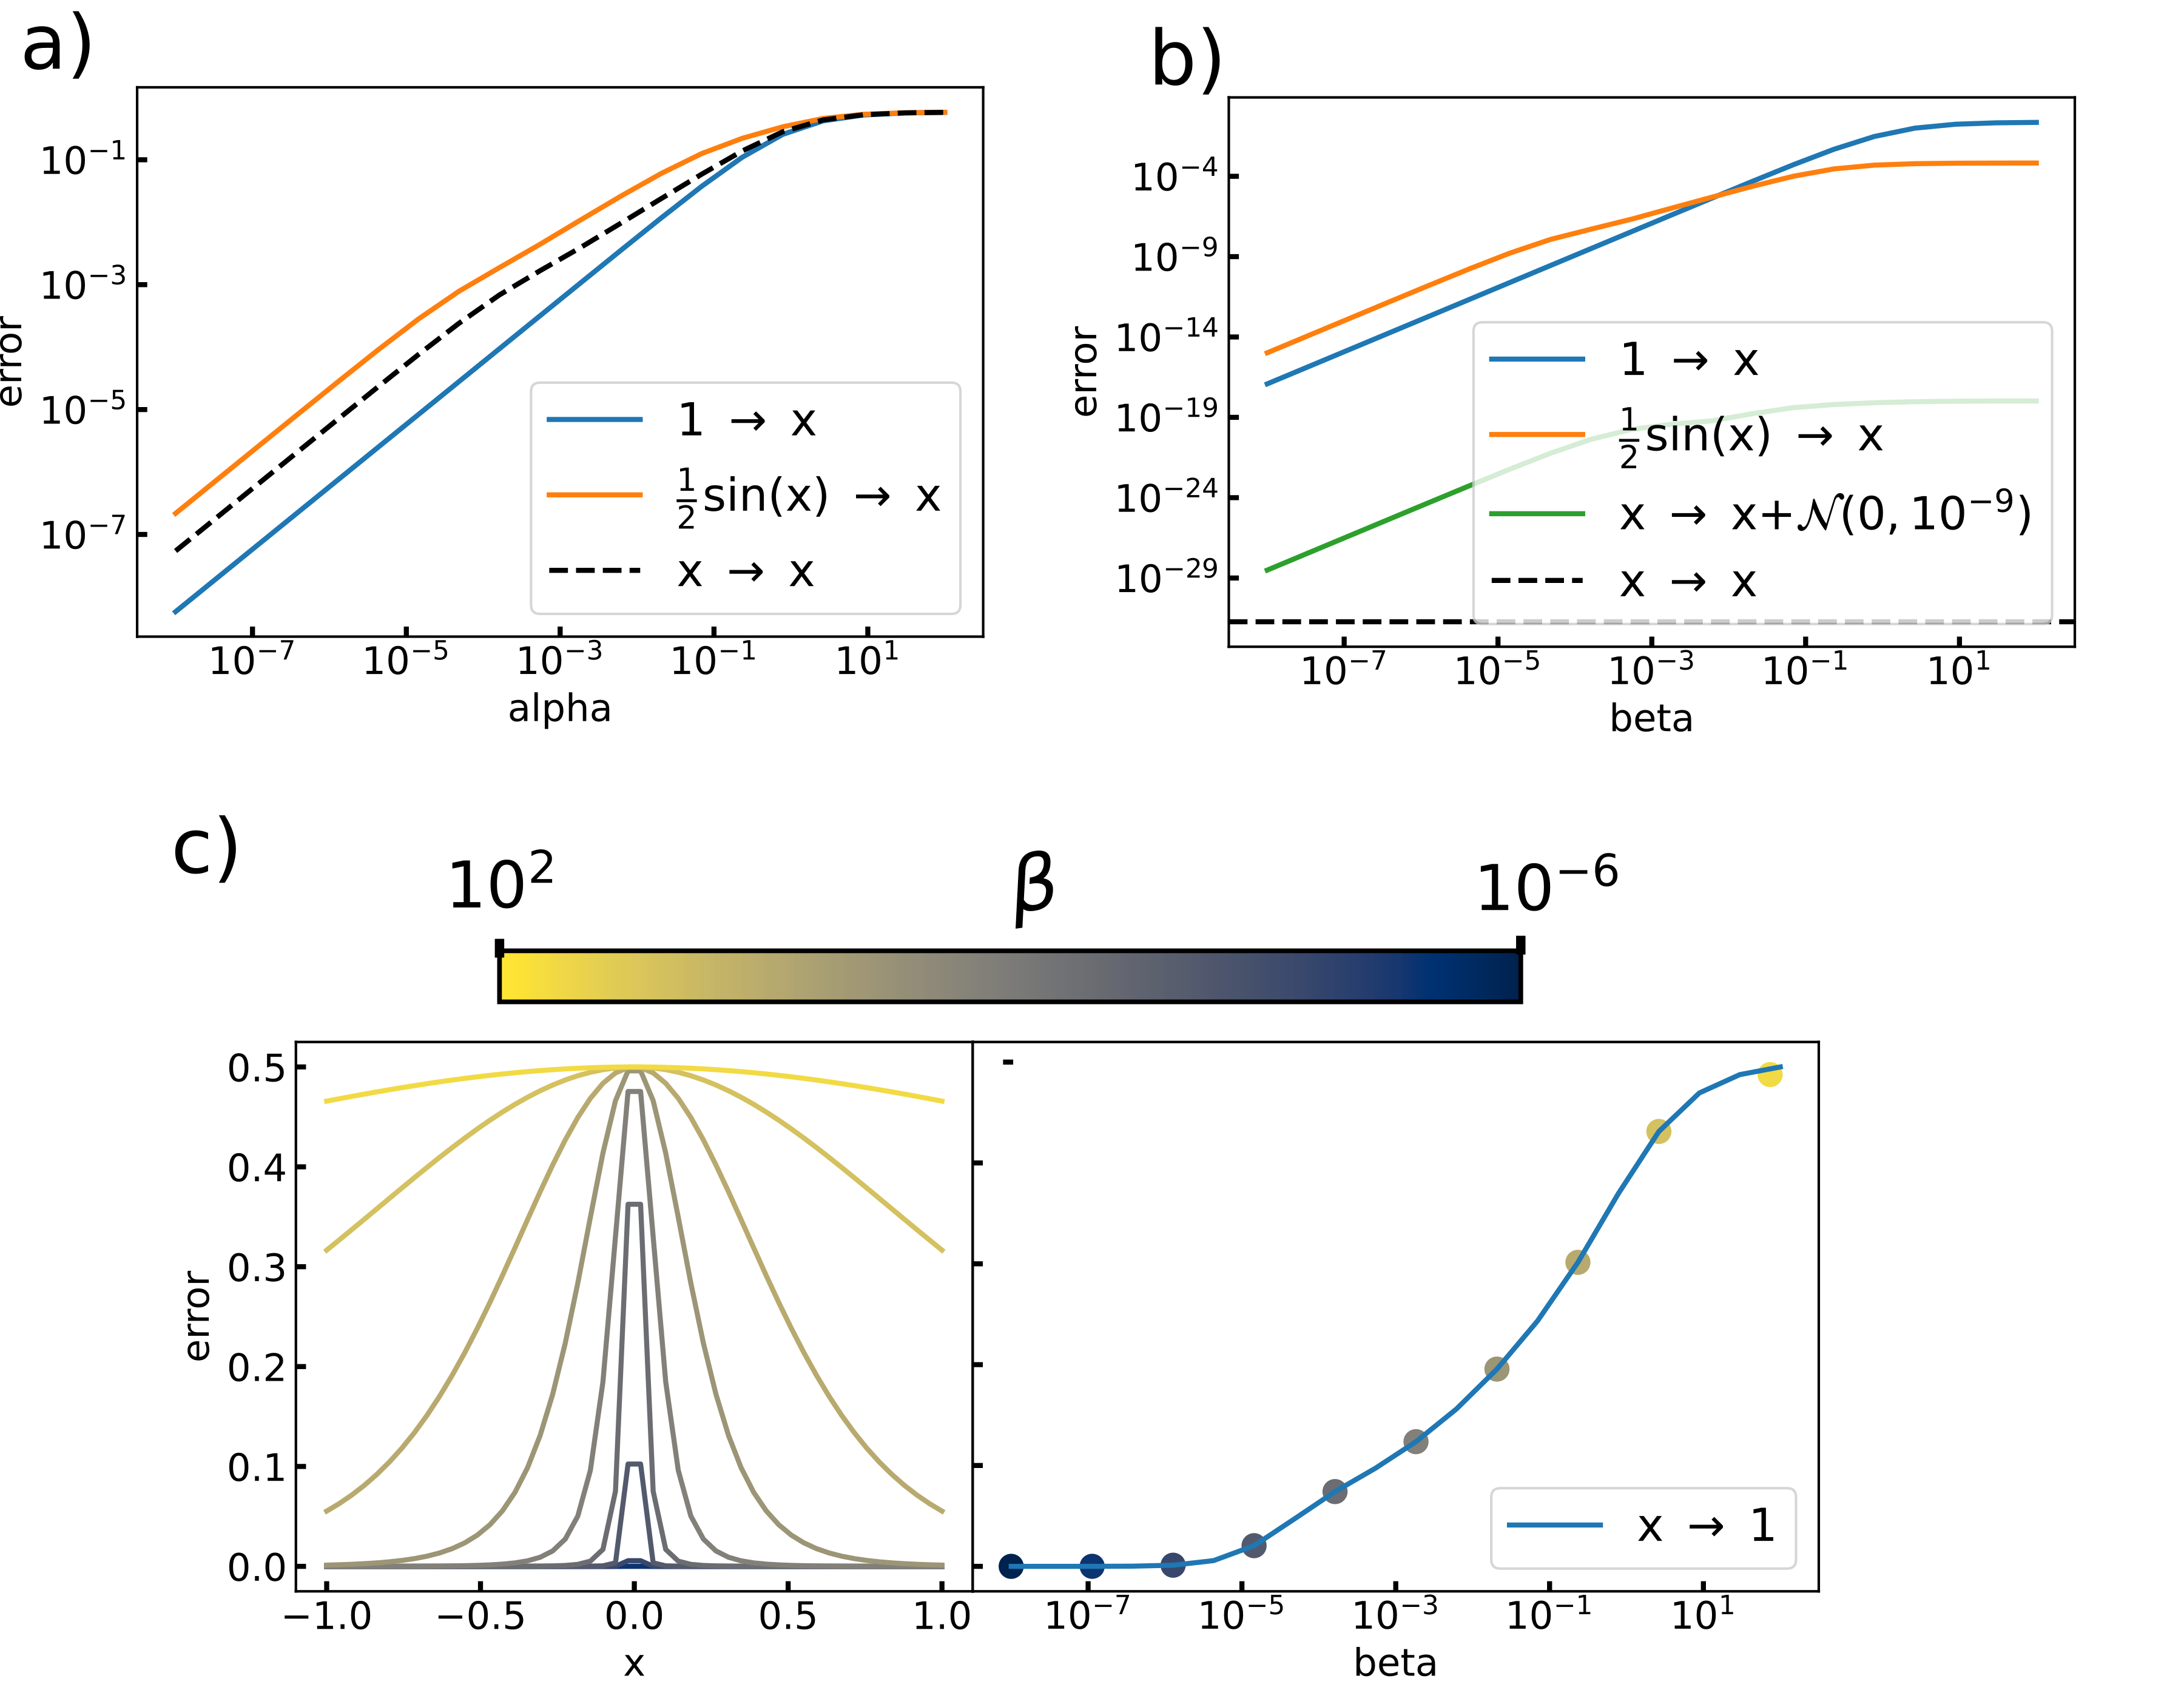
\includegraphics[width=\textwidth]{fig/nonlinear-measure_toy-example.png}
%    \caption{The regression error for the toy dataset $\{x\in [-1,1]\}$ for different features over the spectrum of a) ridge regularization and b) stretch regularization as described in Equation~\eqref{eq:nonlinearm}. c) The error reconstructing the $1$-features from $x$-features for increasing $\beta$ (left) samplewise (right) and averaged over the whole dataset. It can be seen that the error starts to spread starting from the degeneracy at $x=0$.}
%    \label{fig:nonlinearm}
%\end{figure}
%
%While the loss in Equation~\eqref{eq:nonlinearm} is not jointly convex over all $W_i$, it is convex in $W_i$ separately keeping all $W_j$ for $i\neq j$ fixed\cite{LI2015127}.
%We can therefore solve it iteratively until convergence by optimizing in every iteration each weight matrix separately
%\begin{align}
%%&\frac{\partial \ell}{W_i} = 0 \\
%&W_i
%= \big(X_i^TX_i+\beta\sum_{j\neq i}\frac{1}{d(\mathbf{x}_i,\mathbf{x}_j)+1}I)^{-1} \big(X_i^TY_i +  \beta\sum_{j\neq i} \frac{1}{d(\mathbf{x}_i,\mathbf{x}_j)+1} W_j\big)
%\end{align}
%
%With the distance metric $d$, we can induce different degrees of elasticity on the penalty.
%For example by using a Gaussian kernel distances $d_\sigma$ we can control with $\sigma$, how local the penalty should be.
%%An advantage is that with the distance metric we a clear locality in Euclidean space, while the degeneracy approach has an radial scaling the area of effect.
%
%\subsection{Future directions - Restricting nonlinearities}
%
%%Restricting nonlinearities to hierarchical polynomial transformation:
%My interpretation is that $\ell_1$ is the effect of the nonlinearities plus incompleteness and that $\ell_\infty$ is the effect of only incompleteness.
%So $\ell_\infty - \ell_1$ should give us the effect due to nonlinearities.
%In my mind nonlinearities are just Taylor expansions.
%
%%This solves two problems:
%%1. higher body-orders are high-dimensional representation than can heavily truncated, but 
%
%Theoretically speaking there are nonlinearties that cannot be modelled by this approach, but we argue that these are negligible as potentials used in MD are always approximatable.
%%https://math.stackexchange.com/a/1719289
%
%\subsubsection{Future experiment: Effect of incompleteness}
%Information capacity separate the effect of nonlinearities and incompleteness
%\[\ell_{\nu^\prime} = \sum_{\nu^\prime} \overline{\rho^1}^{\nu^\prime} \rightarrow \overline{\rho^{2}}.\]
%Then compare $\ell_1$ with $\ell_\infty$ (sum over $\nu^\prime$ until convergence of error).
%Important: Normalize each body-order separately, and check that the regularizer is very small (like in the range of a jitter to argue that the constant regularization and therefore does not constraint the transformation).
%Repeat result for 3-body potential $f^3$ (like LJ for 3-body) that is well defined over the whole interval
%\[\ell_{\nu^\prime} = \sum_{\nu^\prime} \overline{\rho^1}^{\nu^\prime} \rightarrow f^3\]
%To see if there is any differency the results using the GFRE.
%
%\subsubsection{Future experiment: Charcterizing body-order information in CG-Nets}
%it is super unclear what body orders are actually learning in CG-Net.
%So after each iteration $p$ in the network $f^{(p)}$ we test regression of
%\[\overline{\rho^\nu} \rightarrow f^{(p)}\]
%to see how the body order changes.
%We compare CG-Nets that increase the body order by itself and CG nets that multiply by themselve.
%
%%\[\overline{p^1}+\overline{p^1}^2+\overline{p^1}^3->+\overline{p^3}\]
%%and regression accuracy
%%\[\overline{p^1}+\overline{p^1}^2+\overline{p^1}^3->+\overline{p^3}\]
%%\[\overline{p^1}+\overline{p^1}^2->+\overline{p^2}\]
%
%% bonds
